\documentclass[11pt]{article}
\usepackage[utf8]{inputenc}
\usepackage[T1]{fontenc}
\usepackage{lmodern}
\usepackage[margin=1in]{geometry}
\usepackage{graphicx}
\usepackage{booktabs}
\usepackage{amsmath}
\usepackage{siunitx}
\usepackage{xcolor}
\usepackage{caption}
\captionsetup{font=small,labelfont=bf}
\usepackage[numbers,sort&compress]{natbib}
\usepackage[hidelinks]{hyperref}
\usepackage{orcidlink}
\usepackage{microtype}
% keep every float inside the section that introduces it -- no figures spilling into the bibliography
\usepackage[section]{placeins}

% Vector-figure stack (compile with lualatex). pgfplots panels and the spatial-domain map are
% emitted by manuscript/make_figs.R and \input directly; the schematic is hand-written TikZ.
\usepackage{tikz}
\usepackage{pgfplots}
\pgfplotsset{compat=1.18}
\usepgfplotslibrary{groupplots}
\usetikzlibrary{positioning,arrows.meta,calc,fit,backgrounds}
% shared figure palette -- the named colours referenced by make_figs.R's output
\definecolor{tblue}{RGB}{43,108,176}
\definecolor{tgreen}{RGB}{47,133,90}
\definecolor{torange}{RGB}{221,107,32}
\definecolor{tred}{RGB}{197,48,48}
\definecolor{tgray}{RGB}{160,174,192}
\definecolor{tpurple}{RGB}{107,70,193}

\graphicspath{{figures/}{figs/}}
\title{\vspace{-2em}A causal law for spatial-domain detection:\\
the value of a spatial prior is set by the ground truth's spatial contiguity}
\author{Zeyu Fu\,\orcidlink{0009-0001-8329-0108}\\
State Key Laboratory of Trauma and Chemical Poisoning, Institute of Combined Injury,\\
Chongqing Engineering Research Center for Nanomedicine, College of Preventive Medicine,\\
Army Medical University, Chongqing, China\\
\href{mailto:fuzeyu99@126.com}{fuzeyu99@126.com}}
\date{}

\begin{document}
\maketitle
\vspace{-2em}

\begin{abstract}
\noindent
Methods for spatial-domain detection in spatial transcriptomics are routinely ranked on one or two Visium
datasets under a single clustering backend, and each new paper claims a state-of-the-art. We argue the
reliable object of study is not which method wins but a predictive, causal law for whether a spatial prior
helps at all. On synthetic tissue where we manipulate \emph{only} the ground truth's spatial contiguity---
scrambling positions while holding each cell's expression and label fixed---the advantage of a spatial
prior rises with contiguity and flips sign, at Spearman $\rho=+0.98$ to $+1.00$ ($p<0.001$); because
contiguity is the sole variable changed, this identifies it as the cause rather than a correlate. The same
law holds observationally across eleven technologically diverse datasets: spatial-prior advantage tracks
ground-truth contiguity at Spearman $+0.72$ ($p=0.012$, 95\% CI $[0.24,0.92]$), the only significant
correlation we test; it survives control for cluster count, feature dimension, and assay modality, predicts
held-out datasets, and strengthens under the author-recommended backend. Consistent with a law about tasks
rather than methods, no method is a universal winner: seven different winners across the panel, a clustering
backend that alone re-ranks methods by as much as the entire between-method spread, and a competitive
two-line neighbour-mean floor. A label-free spatial-coherence-gain proxy recovers the direction of the law
(Spearman $+0.55$) but, once we correct for having selected it from six candidates, is a directional,
honestly marginal prior rather than a significant predictor (search-corrected $p=0.28$). The unit of
progress should shift from building a better method to deciding, before committing, whether a spatial prior
is warranted.
\end{abstract}

\noindent\textbf{Keywords:} spatial transcriptomics; spatial-domain detection; benchmarking; clustering;
graph neural networks; method selection; spatial autocorrelation; reproducibility.

\section{Introduction}
Spatial transcriptomics and spatial proteomics assays measure molecular abundance while retaining each
cell's or spot's tissue location \citep{stahl2016st,moffitt2018merfish}. A central unsupervised task is
\emph{spatial-domain detection}: partitioning a tissue into coherent regions such as cortical layers,
anatomical domains, or tumour versus stroma. Most methods encode expression over a spatial nearest-neighbour graph so
that physically adjacent cells obtain similar embeddings, then cluster those embeddings
\citep{dong2022stagate,xu2024sedr,long2023graphst,ren2022spaceflow,hu2021spagcn}.

Two assumptions pervade this literature. First, evaluation is narrow: methods are usually compared
on one or two human-cortex Visium datasets \citep{maynard2021dlpfc} under a single clustering backend, and
a SOTA claim is declared from one adjusted-Rand-index (ARI) table. Second, methods are presented as
universally preferable, with little attention to \emph{when} a spatial prior is appropriate at all.
We argue both framings are wrong. Across technologies, tissues, and ground-truth (GT) types, no method is
consistently best, and which method wins, and indeed whether any spatial method should be used, is
predictable from a single property of the task.

We reframe the question from ``which method wins'' to ``when do spatial priors help, and can we tell in
advance''. Our contributions are:
\begin{itemize}\setlength{\itemsep}{2pt}
\item a \emph{causal, predictive law}: on synthetic tissue where we manipulate contiguity alone, spatial-prior
advantage rises with it and flips sign ($\rho=+0.98$ to $+1.00$, $p<0.001$), and the same law holds
observationally ($\rho=+0.72$, $p=0.012$) as the only correlation we find that is both significant and robust
under our stress tests (\S\ref{sec:law},~\S\ref{sec:causal})---this is the primary result;
\item a label-free spatial-coherence-gain proxy that carries the law to unlabelled tissue, reported honestly
as a directional, marginal prior once its selection among six candidates is corrected for (\S\ref{sec:causal});
\item a confound-controlled, eleven-dataset benchmark showing the clustering backend is a first-order
confound and a trivial neighbour-mean floor is competitive (\S\ref{sec:confound});
\item supporting evidence that there is no universal winner, including a method (SpatialLeiden) whose rank
profile is inverted, best exactly where the deep methods are worst (\S\ref{sec:nosota}); and
\item a worked example, on a candidate method, of how single-dataset evaluation can certify a false SOTA
and a false mechanism (\S\ref{sec:tessera}).
\end{itemize}

\section{Related work}
\paragraph{Spatial-domain methods.} Graph-autoencoder approaches encode expression over a spatial graph:
STAGATE uses a graph-attention autoencoder \citep{dong2022stagate}; SEDR a variational graph autoencoder
with self-supervision \citep{xu2024sedr}. Contrastive and infomax approaches include GraphST
\citep{long2023graphst} and SpaceFlow, which adds spatial regularisation to deep graph infomax
\citep{ren2022spaceflow}. SpaGCN couples a graph convolutional network with histology and a spatially
aware iterative clustering \citep{hu2021spagcn}. Non-deep pipelines include BANKSY, which augments each
cell with neighbourhood features \citep{singhal2024banksy}, and graph-community detection via the Leiden
algorithm \citep{traag2019leiden} on a spatially blended graph.

\paragraph{Benchmarking and backends.} Comparisons typically fix one Visium benchmark
\citep{maynard2021dlpfc} and one clustering backend, often Gaussian mixture model selection via mclust
\citep{scrucca2016mclust}. We show both choices silently re-rank methods.

\paragraph{Benchmarks of spatial-domain detection.} A wave of recent benchmarks scores many methods over many
datasets. Yuan et al.\ (13 methods, 34 samples) \citep{yuan2024benchmark}, Chen et al.\ (14 methods, $\sim$600
real and simulated datasets, with a replicate-consistency axis) \citep{chen2025imeta}, and Kang et al.\ (19
methods, scored jointly with domain-specific spatially variable genes) \citep{kang2025nar} all rank methods by
supervised accuracy against annotated ground truth; Descoeudres, Canzar et al.\ (26 methods) add an explanatory
regression of \emph{why} methods perform well, but still on a supervised-accuracy target
\citep{canzar2026biorxiv}; and Sun et al.\ introduce an unsupervised Smoothness Entropy for expert-guided
consensus and quality control \citep{sun2025smoothness}. All of these rank or explain method performance; none
runs a causal contiguity perturbation, and none validates a label-free proxy against a held-out
spatial-advantage target across platforms. That combination is the wedge of this work
(Table~\ref{tab:related-benchmarks}).

% Differentiation table: tessera-st vs. the 5 directly-overlapping 2024-2026 benchmarks.
\begin{table}[t]
\centering
\caption{Positioning tessera-st's causal-contiguity + label-free-proxy wedge against the five
directly overlapping spatial-domain-detection benchmarks (2024--2026). ``Winner-counting'' denotes
designs that rank methods by supervised accuracy (ARI/NMI-type) against annotated ground truth
without a causal perturbation test or a validated label-free proxy.}
\label{tab:related-benchmarks}
\small
\begin{tabular}{@{}p{2.6cm}p{2.7cm}p{2.5cm}p{3.9cm}p{3.3cm}@{}}
\toprule
Study & Datasets & Methods & Primary axis & Distinct from tessera-st? \\
\midrule
Yuan et al., \textit{Nat. Methods} 2024 \citep{yuan2024benchmark} &
34 real (7 datasets) + 22 hard extension &
13 &
Accuracy, continuity, marker genes, scalability, robustness (winner-counting) &
No causal-perturbation or label-free proxy axis; flags non-contiguous domains as unsolved but does not test causally \\
\addlinespace
Chen et al., \textit{iMeta} 2025 \citep{chen2025imeta} &
$\sim$600 real + simulated (incl.\ replicate sims) &
14 &
Accuracy + replicate/neighborhood-disruption robustness (winner-counting) &
Replicate-consistency $\ne$ causal contiguity; no label-free proxy, no ground-truth-free validation \\
\addlinespace
Kang et al., \textit{NAR} 2025 \citep{kang2025nar} &
30 real (6 platforms) + 27 synthetic &
19 &
Domain accuracy jointly with domain-specific SVG detection; cross-method concordance (winner-counting) &
Concordance $\ne$ causal validity; motivates ensembling, not a mechanistic contiguity test or proxy \\
\addlinespace
Descoeudres/Canzar et al., bioRxiv 2026 \citep{canzar2026biorxiv} &
63 real (6 platforms) + $>$1000 semi-synthetic &
26 &
Explanatory attribution of \emph{why} methods perform well (regression on supervised accuracy) &
Closest ``why'' framing, but target is still supervised accuracy; no causal-contiguity perturbation, no label-free proxy \\
\addlinespace
Sun et al., bioRxiv 2025 \citep{sun2025smoothness} (Smoothness Entropy) &
15 datasets, 9 technologies, 170+ samples &
22 (61 configs) &
Smoothness Entropy / Cross-Method Entropy for expert-guided consensus QC (unsupervised flagging, not proxy validation) &
SE is unsupervised like tessera's coh\_gain, but used for consensus/QC flagging, not correlated against a held-out spatial-advantage target across platforms; no causal sweep \\
\midrule
\textbf{tessera-st (this work)} &
11 platforms (label-free proxy search) + synthetic causal sweep &
6 label-free candidates + causal contiguity generator &
(i) Causal: synthetic contiguity-perturbation sweep, $\rho\!=\!+0.98\text{--}1.00$, $p<0.001$; (ii) Proxy: coh\_gain label-free candidate, observed $\rho=+0.55$, honestly reported as directional/marginal (search-corrected $p=0.28$; uncorrected $p=0.079$) &
Only entry combining a causal ground-truth-free perturbation test with an explicitly falsification-audited label-free proxy, rather than supervised winner-counting \\
\bottomrule
\end{tabular}
\end{table}

\paragraph{Spatial statistics.}
Our predictor is rooted in spatial autocorrelation \citep{moran1950}; clustering agreement is measured
with the adjusted Rand index \citep{hubert1985ari} and normalised mutual information \citep{strehl2002nmi}.
Data handling uses Scanpy \citep{wolf2018scanpy} and Squidpy \citep{palla2022squidpy}.

\section{Methods}\label{sec:methods}
\subsection{Data}
We assemble 11 datasets spanning sequencing- and imaging-based assays, tissues, and
GT types (Table~\ref{tab:data}): DLPFC Visium \citep{maynard2021dlpfc}, seqFISH mouse embryo
\citep{lohoff2022seqfish}, MERFISH hypothalamus \citep{moffitt2018merfish}, STARmap cortex
\citep{wang2018starmap}, osmFISH cortex \citep{codeluppi2018osmfish}, MIBI-TOF \citep{keren2018mibitof},
breast IMC \citep{jackson2020imc}, Open-ST \citep{schott2024openst}, Slide-seqV2 \citep{stickels2021slideseq},
and CODEX spleen \citep{goltsev2018codex}, accessed via Squidpy \citep{palla2022squidpy} where applicable. A review-caught byte-duplicate dataset was removed and a duplicate guard
added, giving $n{=}11$; three additional cancer datasets extend a robustness analysis to
$n{=}14$. Large datasets are deterministically subsampled to 16{,}000 cells (logged). Counts are
library-size normalised and log-transformed; for panels with $>500$ features the top-3000
highly variable genes are retained; features are then $z$-scored and clipped to $[-10,10]$.

\subsection{Methods and backends}
The panel comprises Tessera (the candidate boundary-aware method),
STAGATE, SEDR, GraphST, SpaceFlow, SpaGCN, SpatialLeiden, BANKSY-style neighbour augmentation, and two
floors (non-spatial clustering; neighbour-mean smoothing). SEDR, GraphST, and SpaceFlow run under a no-op
\texttt{numba} shim so they execute on \texttt{numpy}~$\geq$~2.3 without changing the environment; each
brand name is confined to driver scripts (a strict separation enforced by tests). Clustering backends are
KMeans \citep{macqueen1967kmeans} and Gaussian mixtures; for a backend-fairness analysis we add
the clusterer the deep methods recommend, R's \texttt{mclust} \citep{scrucca2016mclust}, called
via an \texttt{Rscript} subprocess (rpy2 does not build in our Python environment, so we round-trip
the embedding through a CSV). Each method is scored at its own best configuration (best over backends
$\times$ \{refinement off, on\}).

\subsection{Metrics and definitions}
We report a full 11-metric panel (ARI, NMI, CHAOS, PAS, ASW, DBI, CAL,
boundary-F1, small-domain IoU, ECE, marker purity), each flagged for circularity, and triangulate rather
than rely on any single metric. We define a GT's \emph{spatial contiguity} as the mean fraction of each
cell's spatial $k$-nearest-neighbours ($k{=}6$) that share its GT label ($1$ = perfectly contiguous,
$\approx 1/K$ = spatially scattered). The \emph{spatial-prior advantage} of a dataset is the best spatial
method's ARI minus the non-spatial floor's ARI. The \emph{label-free} proxy \texttt{coh\_gain} is the gain
in spatial coherence (kNN same-cluster fraction) when unsupervised clustering is run on spatially smoothed
versus raw expression.

\subsection{Statistical analysis}
Correlations use Spearman's $\rho$ with mid-rank ties and asymptotic $p$-values.
Uncertainty is a 10{,}000-resample dataset bootstrap; out-of-sample validity is leave-one-dataset-out
(LODO); confound control uses rank-residual partial correlations against cluster count, effective feature
dimension, and imaging-vs-sequencing modality. The causal experiment manipulates contiguity directly on
synthetic tissue (below). All headline numbers are machine-checked against JSON artifacts by a verifier
script (exit~0).

\begin{table}[htbp]\centering\small
\caption{The 11-dataset panel (plus three cancer datasets for the $n{=}14$ robustness check). Each row is
a distinct published dataset, named by its assay (e.g.\ MERFISH) or tissue (e.g.\ DLPFC). Modality
is the broad measurement class, imaging (FISH/protein) versus sequencing, and is one of the
confounds controlled for in \S\ref{sec:law}. GT contiguity is computed on the (subsampled) data used for
benchmarking.}
\label{tab:data}
\begin{tabular}{lllrrr}
\toprule
Dataset & Modality & GT type & $n$ cells & $K$ & contiguity\\
\midrule
MERFISH      & imaging (FISH)      & domain     & 5{,}488  & 8  & 0.931\\
STARmap      & imaging (FISH)      & region     & 1{,}207  & 7  & 0.921\\
DLPFC        & Visium (seq.)       & layer      & 3{,}639  & 7  & 0.905\\
BRCA         & Visium (seq.)       & tumour     & 3{,}798  & 20 & 0.865\\
osmFISH      & imaging (FISH)      & region     & 5{,}328  & 12 & 0.817\\
IMC          & imaging (protein)   & cell type  & 4{,}668  & 11 & 0.630\\
seqFISH      & imaging (FISH)      & cell type  & 16{,}000 & 22 & 0.621\\
Open-ST       & seq. (3D)           & annotation & 15{,}000 & 14 & 0.562\\
Slide-seqV2  & seq. (bead)         & region     & 16{,}000 & 14 & 0.274\\
MIBI-TOF     & imaging (protein)   & cluster    & 3{,}309  & 8  & 0.271\\
CODEX        & imaging (protein)   & niche      & 16{,}000 & 100& 0.022\\
\midrule
st\_OV / st\_COAD / st\_LIHC & cancer ST & cell type & 16{,}000 & 13--19 & 0.69/0.50/0.22\\
\bottomrule
\end{tabular}
\end{table}

\section{The backend is a confound, and a trivial baseline is competitive}\label{sec:confound}
Switching KMeans${\to}$GMM changes a single method's cross-section ARI by 0.036--0.200; the largest shift
(STAGATE, 0.20) approximately equals the full between-method ARI spread of $0.494-0.291=0.203$, so a
benchmark that fixes one backend re-ranks methods. That headline spread is anchored to GraphST (0.291),
a baseline our Limitations (\S\ref{sec:limitations}) flags as under-tuned and hence a lower bound on its
true ARI; excluding it, the spread among the remaining six methods is $0.494-0.344=0.150$ (set by
\texttt{floor:nonspatial}), which no longer matches the largest single-backend shift. The re-ranking claim
is therefore robust, but the specific ``shift equals spread'' framing is sensitive to retaining the
under-tuned baseline.

A two-line neighbour-mean floor reaches cross-section ARI 0.473 (rank 3/7,
within 0.03 of the best deep method, Table~\ref{tab:backend}): new methods should be required to beat
neighbour-mean, not merely non-spatial clustering.

\begin{table}[htbp]\centering\small
\caption{The clustering backend is a first-order confound, and a parameter-free neighbour-mean floor is
competitive. $\Delta$ARI is the per-method shift from KMeans to GMM (averaged over three DLPFC donors);
cross-section ARI is the mean$\pm$std over donors under a unified GMM backend. The full between-method ARI
spread, $0.494-0.291=0.203$ (STAGATE to GraphST), approximately equals the largest single backend shift
(STAGATE, 0.200); but GraphST is the under-tuned baseline flagged in Limitations, so its 0.291 is a lower
bound, and excluding it the spread among the remaining six methods is only $0.494-0.344=0.150$
(STAGATE to \texttt{floor:nonspatial}) -- below the largest single shift. \texttt{floor:smoothed} ranks
third either way.}
\label{tab:backend}
\begin{tabular}{lcc}
\toprule
Method & $\Delta$ARI(GMM$-$KMeans) & cross-section ARI\\
\midrule
STAGATE          & 0.200 & $0.494\pm0.087$\\
SEDR             & 0.170 & $0.483\pm0.056$\\
\textbf{floor:smoothed} & 0.164 & $\mathbf{0.473\pm0.055}$\\
BANKSY-style     & 0.149 & $0.450\pm0.032$\\
Tessera          & \textbf{0.036} & $0.392\pm0.082$\\
floor:nonspatial & 0.166 & $0.344\pm0.061$\\
GraphST          & 0.099 & $0.291\pm0.042$\\
\bottomrule
\end{tabular}
\end{table}

\begin{figure}[htbp]\centering
\resizebox{\linewidth}{!}{% !TEX encoding = UTF-8 Unicode
\begin{tikzpicture}[x=1pt,y=1pt]
\definecolor{fillColor}{RGB}{255,255,255}
\path[use as bounding box,fill=fillColor,fill opacity=0.00] (0,0) rectangle (472.86,130.39);
\begin{scope}
\path[clip] (  2.89,  2.89) rectangle (469.96,127.50);

\path[] (  2.89,  2.89) rectangle (469.96,127.50);
\end{scope}
\begin{scope}
\path[clip] (  4.89,  4.89) rectangle (116.91,116.91);
\node[inner sep=0pt,outer sep=0pt,anchor=south west,rotate=  0.00] at (  4.89,   4.89) {
	\pgfimage[width=112.02pt,height=112.02pt,interpolate=true]{figs/fig_spatialmap_ras1}};
\end{scope}
\begin{scope}
\path[clip] (121.91,  4.89) rectangle (233.93,116.91);
\node[inner sep=0pt,outer sep=0pt,anchor=south west,rotate=  0.00] at (121.91,   4.89) {
	\pgfimage[width=112.02pt,height=112.02pt,interpolate=true]{figs/fig_spatialmap_ras2}};
\end{scope}
\begin{scope}
\path[clip] (238.93,  4.89) rectangle (350.95,116.91);
\node[inner sep=0pt,outer sep=0pt,anchor=south west,rotate=  0.00] at (238.93,   4.89) {
	\pgfimage[width=112.02pt,height=112.02pt,interpolate=true]{figs/fig_spatialmap_ras3}};
\end{scope}
\begin{scope}
\path[clip] (355.95,  4.89) rectangle (467.96,116.91);
\node[inner sep=0pt,outer sep=0pt,anchor=south west,rotate=  0.00] at (355.95,   4.89) {
	\pgfimage[width=112.02pt,height=112.02pt,interpolate=true]{figs/fig_spatialmap_ras4}};
\end{scope}
\begin{scope}
\path[clip] (  4.89,116.91) rectangle (116.91,125.50);
\definecolor{drawColor}{RGB}{0,0,0}

\node[text=drawColor,anchor=base,inner sep=0pt, outer sep=0pt, scale=  0.70] at ( 60.90,119.79) {(A) ground truth};
\end{scope}
\begin{scope}
\path[clip] (121.91,116.91) rectangle (233.93,125.50);
\definecolor{drawColor}{RGB}{0,0,0}

\node[text=drawColor,anchor=base,inner sep=0pt, outer sep=0pt, scale=  0.70] at (177.92,119.79) {(B) non-spatial KMeans (ARI 0.25)};
\end{scope}
\begin{scope}
\path[clip] (238.93,116.91) rectangle (350.95,125.50);
\definecolor{drawColor}{RGB}{0,0,0}

\node[text=drawColor,anchor=base,inner sep=0pt, outer sep=0pt, scale=  0.70] at (294.94,119.79) {(C) neighbour-mean (ARI 0.96)};
\end{scope}
\begin{scope}
\path[clip] (355.95,116.91) rectangle (467.96,125.50);
\definecolor{drawColor}{RGB}{0,0,0}

\node[text=drawColor,anchor=base,inner sep=0pt, outer sep=0pt, scale=  0.70] at (411.96,119.79) {(D) predicted seams};
\end{scope}
\end{tikzpicture}
}
\caption{Why a spatial prior helps when the ground truth is contiguous (synthetic tessellation,
signal-to-noise tuned so space is necessary). A non-spatial KMeans scatters the contiguous domains while a
parameter-free neighbour-mean smoother recovers them (each panel title gives its ARI); the predicted seams
(right) are an explicit output of the smoother rather than a by-product of the argmax.}
\label{fig:spatialmap}
\end{figure}

\section{No universal winner across methods}\label{sec:nosota}
Across the 11 datasets there are seven distinct winners (Fig.~\ref{fig:heatmap}), becoming eight once
SpaGCN, the most-cited method, is added: it wins only one dataset (Open-ST, by a within-noise 0.005
margin), never becoming universal. The bare count is only modestly above the 6.16 winners expected under a uniform-random-winner null
(\texttt{experiments/robustness\_audit.py}), so the evidence for no-universal-SOTA is not the count but the
shifting winner in the heatmap and the rank inversions below.

The pattern is not an artifact of how the most-cited method is run. The same holds when SpaGCN uses its
genuine native louvain pipeline rather than the fallback: it then runs on 7 of 11 datasets and still wins
only Open-ST, with the same inverted profile. SpatialLeiden's rank profile is inverted too
(Fig.~\ref{fig:profile}): it ranks first or second on the four lowest-contiguity datasets yet last on the
most contiguous, MERFISH. A graph-community method thus excels exactly where the autoencoder and
contrastive methods fail.

Even the apparent winner of the easiest regime is unstable. At the top of the contiguous-task leaderboard
the winner is a tie within seed noise: across three runs the MERFISH winner flipped SpaceFlow, Tessera,
then SpaceFlow again. No single method is reliably best here (Table~\ref{tab:perdataset}).

\begin{table}[htbp]\centering\small
\caption{Per-dataset best-config results (core panel of six methods plus two floors, 3 seeds), ordered by
GT contiguity. The winner differs across datasets (seven distinct winners, one of them a floor), the
spatial-prior advantage tracks contiguity, and the candidate method's rank does not. Winner ARI is the
winner's best-config mean.}
\label{tab:perdataset}
\begin{tabular}{lcclcc}
\toprule
Dataset & contiguity & winner & winner ARI & spatial adv. & Tessera rank\\
\midrule
MERFISH & 0.931 & SpaceFlow & 0.429 & $+0.314$ & 2\\
STARmap & 0.921 & SEDR & 0.579 & $+0.168$ & 5\\
DLPFC & 0.905 & SEDR & 0.584 & $+0.101$ & 2\\
BRCA & 0.865 & STAGATE & 0.616 & $+0.042$ & 2\\
osmFISH & 0.817 & \textbf{Tessera} & 0.438 & $+0.196$ & \textbf{1}\\
IMC & 0.630 & SEDR & 0.485 & $+0.139$ & 8\\
seqFISH & 0.621 & floor:nonspatial & 0.407 & $-0.005$ & 8\\
Open-ST & 0.562 & floor:nonspatial & 0.264 & $-0.005$ & 5\\
Slide-seqV2 & 0.274 & SEDR & 0.118 & $+0.008$ & 4\\
MIBI-TOF & 0.271 & BANKSY-style & 0.247 & $+0.022$ & 5\\
CODEX & 0.022 & SpatialLeiden & 0.081 & $+0.024$ & 3\\
\bottomrule
\end{tabular}

\end{table}

\begin{figure}[htbp]\centering
\resizebox{0.95\linewidth}{!}{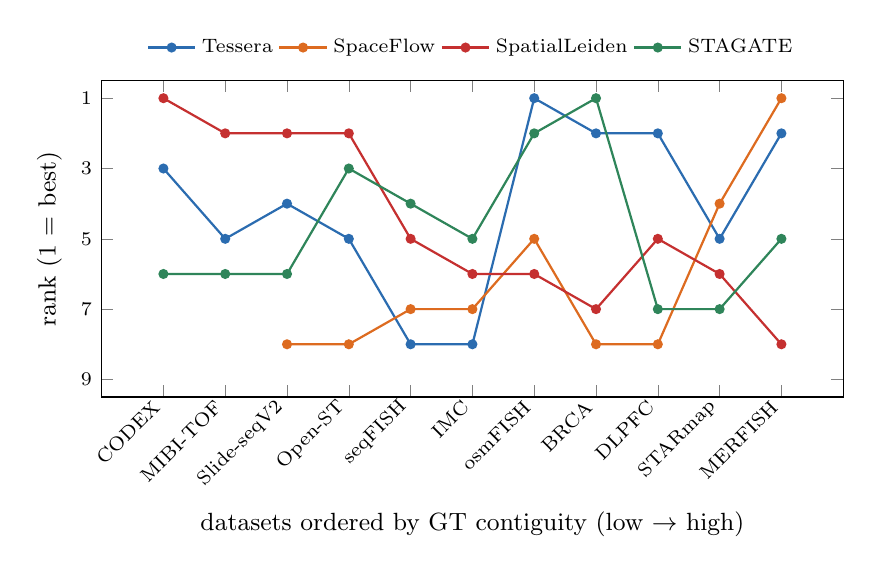
\begin{tikzpicture}
\begin{axis}[width=11cm, height=5.6cm, y dir=reverse, ymin=0.5, ymax=9.5,xtick={0,1,2,3,4,5,6,7,8,9,10}, xticklabels={CODEX,MIBI-TOF,Slide-seqV2,Open-ST,seqFISH,IMC,osmFISH,BRCA,DLPFC,STARmap,MERFISH}, x tick label style={rotate=45, anchor=east, font=\scriptsize},ytick={1,3,5,7,9}, ylabel={rank (1 = best)}, ylabel style={font=\small},xlabel={datasets ordered by GT contiguity (low $\rightarrow$ high)}, xlabel style={font=\small},tick label style={font=\scriptsize}, legend style={font=\scriptsize, at={(0.5,1.04)}, anchor=south, legend columns=4, draw=none}, legend cell align=left]
\addplot[color=tblue, mark=*, mark size=1.4pt, thick] coordinates {
  (0,3)
  (1,5)
  (2,4)
  (3,5)
  (4,8)
  (5,8)
  (6,1)
  (7,2)
  (8,2)
  (9,5)
  (10,2)
};
\addlegendentry{Tessera}
\addplot[color=torange, mark=*, mark size=1.4pt, thick] coordinates {
  (2,8)
  (3,8)
  (4,7)
  (5,7)
  (6,5)
  (7,8)
  (8,8)
  (9,4)
  (10,1)
};
\addlegendentry{SpaceFlow}
\addplot[color=tred, mark=*, mark size=1.4pt, thick] coordinates {
  (0,1)
  (1,2)
  (2,2)
  (3,2)
  (4,5)
  (5,6)
  (6,6)
  (7,7)
  (8,5)
  (9,6)
  (10,8)
};
\addlegendentry{SpatialLeiden}
\addplot[color=tgreen, mark=*, mark size=1.4pt, thick] coordinates {
  (0,6)
  (1,6)
  (2,6)
  (3,3)
  (4,4)
  (5,5)
  (6,2)
  (7,1)
  (8,7)
  (9,7)
  (10,5)
};
\addlegendentry{STAGATE}
\end{axis}
\end{tikzpicture}
}
\caption{Per-method rank versus GT contiguity. Method--task fit is method-specific: SpatialLeiden's profile
is inverted (wins low-contiguity datasets, last on high-contiguity MERFISH).}
\label{fig:profile}
\end{figure}

\begin{figure}[htbp]\centering
\resizebox{\linewidth}{!}{% !TEX encoding = UTF-8 Unicode
\begin{tikzpicture}[x=1pt,y=1pt]
\definecolor{fillColor}{RGB}{255,255,255}
\path[use as bounding box,fill=fillColor,fill opacity=0.00] (0,0) rectangle (516.73,440.85);
\begin{scope}
\path[clip] (  0.00,  0.00) rectangle (516.73,440.85);
\definecolor{drawColor}{RGB}{255,255,255}
\definecolor{fillColor}{RGB}{255,255,255}

\path[draw=drawColor,line width= 0.6pt,line join=round,line cap=round,fill=fillColor] (  0.00,  0.00) rectangle (516.73,440.85);
\end{scope}
\begin{scope}
\path[clip] (  5.50,202.03) rectangle (256.11,435.35);
\definecolor{fillColor}{RGB}{255,255,255}

\path[fill=fillColor] (  5.50,202.03) rectangle (256.11,435.35);
\end{scope}
\begin{scope}
\path[clip] (256.11,202.03) rectangle (511.23,435.35);
\definecolor{fillColor}{RGB}{255,255,255}

\path[fill=fillColor] (256.11,202.03) rectangle (511.23,435.35);
\end{scope}
\begin{scope}
\path[clip] (  5.50,  5.50) rectangle (256.11,202.03);
\definecolor{fillColor}{RGB}{255,255,255}

\path[fill=fillColor] (  5.50,  5.50) rectangle (256.11,202.03);
\end{scope}
\begin{scope}
\path[clip] (256.11,  5.50) rectangle (511.23,202.03);
\definecolor{fillColor}{RGB}{255,255,255}

\path[fill=fillColor] (256.11,  5.50) rectangle (511.23,202.03);
\end{scope}
\begin{scope}
\path[clip] ( 61.30,266.12) rectangle (252.11,414.55);
\definecolor{drawColor}{gray}{0.92}

\path[draw=drawColor,line width= 0.4pt,line join=round] ( 61.30,276.98) --
	(252.11,276.98);

\path[draw=drawColor,line width= 0.4pt,line join=round] ( 61.30,295.08) --
	(252.11,295.08);

\path[draw=drawColor,line width= 0.4pt,line join=round] ( 61.30,313.18) --
	(252.11,313.18);

\path[draw=drawColor,line width= 0.4pt,line join=round] ( 61.30,331.28) --
	(252.11,331.28);

\path[draw=drawColor,line width= 0.4pt,line join=round] ( 61.30,349.38) --
	(252.11,349.38);

\path[draw=drawColor,line width= 0.4pt,line join=round] ( 61.30,367.49) --
	(252.11,367.49);

\path[draw=drawColor,line width= 0.4pt,line join=round] ( 61.30,385.59) --
	(252.11,385.59);

\path[draw=drawColor,line width= 0.4pt,line join=round] ( 61.30,403.69) --
	(252.11,403.69);

\path[draw=drawColor,line width= 0.4pt,line join=round] ( 71.52,266.12) --
	( 71.52,414.55);

\path[draw=drawColor,line width= 0.4pt,line join=round] ( 88.55,266.12) --
	( 88.55,414.55);

\path[draw=drawColor,line width= 0.4pt,line join=round] (105.59,266.12) --
	(105.59,414.55);

\path[draw=drawColor,line width= 0.4pt,line join=round] (122.63,266.12) --
	(122.63,414.55);

\path[draw=drawColor,line width= 0.4pt,line join=round] (139.67,266.12) --
	(139.67,414.55);

\path[draw=drawColor,line width= 0.4pt,line join=round] (156.70,266.12) --
	(156.70,414.55);

\path[draw=drawColor,line width= 0.4pt,line join=round] (173.74,266.12) --
	(173.74,414.55);

\path[draw=drawColor,line width= 0.4pt,line join=round] (190.78,266.12) --
	(190.78,414.55);

\path[draw=drawColor,line width= 0.4pt,line join=round] (207.81,266.12) --
	(207.81,414.55);

\path[draw=drawColor,line width= 0.4pt,line join=round] (224.85,266.12) --
	(224.85,414.55);

\path[draw=drawColor,line width= 0.4pt,line join=round] (241.89,266.12) --
	(241.89,414.55);
\definecolor{drawColor}{RGB}{255,255,255}
\definecolor{fillColor}{RGB}{255,218,159}

\path[draw=drawColor,line width= 0.2pt,fill=fillColor] ( 97.07,394.64) rectangle (114.11,412.74);
\definecolor{fillColor}{RGB}{195,61,113}

\path[draw=drawColor,line width= 0.2pt,fill=fillColor] (199.29,394.64) rectangle (216.33,412.74);
\definecolor{fillColor}{RGB}{234,106,106}

\path[draw=drawColor,line width= 0.2pt,fill=fillColor] (131.15,394.64) rectangle (148.18,412.74);
\definecolor{fillColor}{RGB}{255,196,140}

\path[draw=drawColor,line width= 0.2pt,fill=fillColor] (233.37,394.64) rectangle (250.41,412.74);
\definecolor{fillColor}{RGB}{240,123,107}

\path[draw=drawColor,line width= 0.2pt,fill=fillColor] (182.26,394.64) rectangle (199.29,412.74);
\definecolor{fillColor}{RGB}{51,16,94}

\path[draw=drawColor,line width= 0.2pt,fill=fillColor] (148.18,394.64) rectangle (165.22,412.74);
\definecolor{fillColor}{RGB}{253,246,185}

\path[draw=drawColor,line width= 0.2pt,fill=fillColor] ( 63.00,394.64) rectangle ( 80.04,412.74);
\definecolor{fillColor}{RGB}{47,16,84}

\path[draw=drawColor,line width= 0.2pt,fill=fillColor] (114.11,394.64) rectangle (131.15,412.74);
\definecolor{fillColor}{RGB}{144,42,128}

\path[draw=drawColor,line width= 0.2pt,fill=fillColor] (165.22,394.64) rectangle (182.26,412.74);
\definecolor{fillColor}{RGB}{51,16,93}

\path[draw=drawColor,line width= 0.2pt,fill=fillColor] (216.33,394.64) rectangle (233.37,412.74);
\definecolor{fillColor}{RGB}{28,13,44}

\path[draw=drawColor,line width= 0.2pt,fill=fillColor] ( 80.04,394.64) rectangle ( 97.07,412.74);
\definecolor{fillColor}{RGB}{244,133,108}

\path[draw=drawColor,line width= 0.2pt,fill=fillColor] ( 97.07,376.54) rectangle (114.11,394.64);
\definecolor{fillColor}{RGB}{215,70,106}

\path[draw=drawColor,line width= 0.2pt,fill=fillColor] (199.29,376.54) rectangle (216.33,394.64);
\definecolor{fillColor}{RGB}{108,29,122}

\path[draw=drawColor,line width= 0.2pt,fill=fillColor] (131.15,376.54) rectangle (148.18,394.64);
\definecolor{fillColor}{RGB}{236,113,107}

\path[draw=drawColor,line width= 0.2pt,fill=fillColor] (233.37,376.54) rectangle (250.41,394.64);
\definecolor{fillColor}{RGB}{239,119,107}

\path[draw=drawColor,line width= 0.2pt,fill=fillColor] (182.26,376.54) rectangle (199.29,394.64);
\definecolor{fillColor}{RGB}{35,15,59}

\path[draw=drawColor,line width= 0.2pt,fill=fillColor] (148.18,376.54) rectangle (165.22,394.64);
\definecolor{fillColor}{RGB}{252,253,191}

\path[draw=drawColor,line width= 0.2pt,fill=fillColor] ( 63.00,376.54) rectangle ( 80.04,394.64);
\definecolor{fillColor}{RGB}{91,24,118}

\path[draw=drawColor,line width= 0.2pt,fill=fillColor] (114.11,376.54) rectangle (131.15,394.64);
\definecolor{fillColor}{RGB}{145,42,128}

\path[draw=drawColor,line width= 0.2pt,fill=fillColor] (165.22,376.54) rectangle (182.26,394.64);
\definecolor{fillColor}{RGB}{42,16,73}

\path[draw=drawColor,line width= 0.2pt,fill=fillColor] (216.33,376.54) rectangle (233.37,394.64);
\definecolor{fillColor}{RGB}{1,0,6}

\path[draw=drawColor,line width= 0.2pt,fill=fillColor] ( 80.04,376.54) rectangle ( 97.07,394.64);
\definecolor{fillColor}{RGB}{255,229,169}

\path[draw=drawColor,line width= 0.2pt,fill=fillColor] ( 97.07,322.23) rectangle (114.11,340.33);
\definecolor{fillColor}{RGB}{231,97,106}

\path[draw=drawColor,line width= 0.2pt,fill=fillColor] (199.29,322.23) rectangle (216.33,340.33);
\definecolor{fillColor}{RGB}{103,27,121}

\path[draw=drawColor,line width= 0.2pt,fill=fillColor] (131.15,322.23) rectangle (148.18,340.33);
\definecolor{fillColor}{RGB}{255,225,165}

\path[draw=drawColor,line width= 0.2pt,fill=fillColor] (233.37,322.23) rectangle (250.41,340.33);
\definecolor{fillColor}{RGB}{184,57,117}

\path[draw=drawColor,line width= 0.2pt,fill=fillColor] (182.26,322.23) rectangle (199.29,340.33);
\definecolor{fillColor}{RGB}{99,26,120}

\path[draw=drawColor,line width= 0.2pt,fill=fillColor] (148.18,322.23) rectangle (165.22,340.33);
\definecolor{fillColor}{RGB}{255,221,162}

\path[draw=drawColor,line width= 0.2pt,fill=fillColor] ( 63.00,322.23) rectangle ( 80.04,340.33);
\definecolor{fillColor}{RGB}{252,154,109}

\path[draw=drawColor,line width= 0.2pt,fill=fillColor] (114.11,322.23) rectangle (131.15,340.33);
\definecolor{fillColor}{RGB}{145,42,128}

\path[draw=drawColor,line width= 0.2pt,fill=fillColor] (165.22,322.23) rectangle (182.26,340.33);
\definecolor{fillColor}{RGB}{56,15,106}

\path[draw=drawColor,line width= 0.2pt,fill=fillColor] (216.33,322.23) rectangle (233.37,340.33);
\definecolor{fillColor}{RGB}{27,13,43}

\path[draw=drawColor,line width= 0.2pt,fill=fillColor] ( 80.04,322.23) rectangle ( 97.07,340.33);
\definecolor{fillColor}{RGB}{204,65,110}

\path[draw=drawColor,line width= 0.2pt,fill=fillColor] ( 97.07,340.33) rectangle (114.11,358.44);
\definecolor{fillColor}{RGB}{197,62,112}

\path[draw=drawColor,line width= 0.2pt,fill=fillColor] (199.29,340.33) rectangle (216.33,358.44);
\definecolor{fillColor}{RGB}{238,117,107}

\path[draw=drawColor,line width= 0.2pt,fill=fillColor] (131.15,340.33) rectangle (148.18,358.44);
\definecolor{fillColor}{RGB}{255,198,142}

\path[draw=drawColor,line width= 0.2pt,fill=fillColor] (233.37,340.33) rectangle (250.41,358.44);
\definecolor{fillColor}{RGB}{227,87,105}

\path[draw=drawColor,line width= 0.2pt,fill=fillColor] (182.26,340.33) rectangle (199.29,358.44);
\definecolor{fillColor}{RGB}{226,86,105}

\path[draw=drawColor,line width= 0.2pt,fill=fillColor] ( 63.00,340.33) rectangle ( 80.04,358.44);
\definecolor{fillColor}{RGB}{60,15,112}

\path[draw=drawColor,line width= 0.2pt,fill=fillColor] (114.11,340.33) rectangle (131.15,358.44);
\definecolor{fillColor}{RGB}{103,27,121}

\path[draw=drawColor,line width= 0.2pt,fill=fillColor] (165.22,340.33) rectangle (182.26,358.44);
\definecolor{fillColor}{RGB}{38,15,65}

\path[draw=drawColor,line width= 0.2pt,fill=fillColor] (216.33,340.33) rectangle (233.37,358.44);
\definecolor{fillColor}{RGB}{253,156,109}

\path[draw=drawColor,line width= 0.2pt,fill=fillColor] ( 97.07,358.44) rectangle (114.11,376.54);
\definecolor{fillColor}{RGB}{211,68,108}

\path[draw=drawColor,line width= 0.2pt,fill=fillColor] (199.29,358.44) rectangle (216.33,376.54);
\definecolor{fillColor}{RGB}{51,16,94}

\path[draw=drawColor,line width= 0.2pt,fill=fillColor] (131.15,358.44) rectangle (148.18,376.54);
\definecolor{fillColor}{RGB}{253,156,109}

\path[draw=drawColor,line width= 0.2pt,fill=fillColor] (233.37,358.44) rectangle (250.41,376.54);
\definecolor{fillColor}{RGB}{193,60,114}

\path[draw=drawColor,line width= 0.2pt,fill=fillColor] (182.26,358.44) rectangle (199.29,376.54);
\definecolor{fillColor}{RGB}{132,38,127}

\path[draw=drawColor,line width= 0.2pt,fill=fillColor] (148.18,358.44) rectangle (165.22,376.54);
\definecolor{fillColor}{RGB}{255,204,147}

\path[draw=drawColor,line width= 0.2pt,fill=fillColor] ( 63.00,358.44) rectangle ( 80.04,376.54);
\definecolor{fillColor}{RGB}{70,17,114}

\path[draw=drawColor,line width= 0.2pt,fill=fillColor] (114.11,358.44) rectangle (131.15,376.54);
\definecolor{fillColor}{RGB}{148,43,127}

\path[draw=drawColor,line width= 0.2pt,fill=fillColor] (165.22,358.44) rectangle (182.26,376.54);
\definecolor{fillColor}{RGB}{54,16,101}

\path[draw=drawColor,line width= 0.2pt,fill=fillColor] (216.33,358.44) rectangle (233.37,376.54);
\definecolor{fillColor}{RGB}{41,16,72}

\path[draw=drawColor,line width= 0.2pt,fill=fillColor] ( 80.04,358.44) rectangle ( 97.07,376.54);
\definecolor{fillColor}{RGB}{254,160,109}

\path[draw=drawColor,line width= 0.2pt,fill=fillColor] ( 97.07,267.93) rectangle (114.11,286.03);
\definecolor{fillColor}{RGB}{219,72,105}

\path[draw=drawColor,line width= 0.2pt,fill=fillColor] (199.29,267.93) rectangle (216.33,286.03);
\definecolor{fillColor}{RGB}{110,30,122}

\path[draw=drawColor,line width= 0.2pt,fill=fillColor] (131.15,267.93) rectangle (148.18,286.03);
\definecolor{fillColor}{RGB}{255,222,163}

\path[draw=drawColor,line width= 0.2pt,fill=fillColor] (233.37,267.93) rectangle (250.41,286.03);
\definecolor{fillColor}{RGB}{231,99,106}

\path[draw=drawColor,line width= 0.2pt,fill=fillColor] (182.26,267.93) rectangle (199.29,286.03);
\definecolor{fillColor}{RGB}{140,41,129}

\path[draw=drawColor,line width= 0.2pt,fill=fillColor] (148.18,267.93) rectangle (165.22,286.03);
\definecolor{fillColor}{RGB}{255,228,169}

\path[draw=drawColor,line width= 0.2pt,fill=fillColor] ( 63.00,267.93) rectangle ( 80.04,286.03);
\definecolor{fillColor}{RGB}{170,51,121}

\path[draw=drawColor,line width= 0.2pt,fill=fillColor] (114.11,267.93) rectangle (131.15,286.03);
\definecolor{fillColor}{RGB}{138,40,129}

\path[draw=drawColor,line width= 0.2pt,fill=fillColor] (165.22,267.93) rectangle (182.26,286.03);
\definecolor{fillColor}{RGB}{42,16,73}

\path[draw=drawColor,line width= 0.2pt,fill=fillColor] (216.33,267.93) rectangle (233.37,286.03);
\definecolor{fillColor}{RGB}{24,11,36}

\path[draw=drawColor,line width= 0.2pt,fill=fillColor] ( 80.04,267.93) rectangle ( 97.07,286.03);
\definecolor{fillColor}{RGB}{252,153,109}

\path[draw=drawColor,line width= 0.2pt,fill=fillColor] ( 97.07,286.03) rectangle (114.11,304.13);
\definecolor{fillColor}{RGB}{232,101,106}

\path[draw=drawColor,line width= 0.2pt,fill=fillColor] (199.29,286.03) rectangle (216.33,304.13);
\definecolor{fillColor}{RGB}{55,16,103}

\path[draw=drawColor,line width= 0.2pt,fill=fillColor] (131.15,286.03) rectangle (148.18,304.13);
\definecolor{fillColor}{RGB}{233,104,106}

\path[draw=drawColor,line width= 0.2pt,fill=fillColor] (233.37,286.03) rectangle (250.41,304.13);
\definecolor{fillColor}{RGB}{136,40,128}

\path[draw=drawColor,line width= 0.2pt,fill=fillColor] (182.26,286.03) rectangle (199.29,304.13);
\definecolor{fillColor}{RGB}{126,36,126}

\path[draw=drawColor,line width= 0.2pt,fill=fillColor] (148.18,286.03) rectangle (165.22,304.13);
\definecolor{fillColor}{RGB}{255,221,162}

\path[draw=drawColor,line width= 0.2pt,fill=fillColor] ( 63.00,286.03) rectangle ( 80.04,304.13);
\definecolor{fillColor}{RGB}{206,66,109}

\path[draw=drawColor,line width= 0.2pt,fill=fillColor] (114.11,286.03) rectangle (131.15,304.13);
\definecolor{fillColor}{RGB}{151,45,126}

\path[draw=drawColor,line width= 0.2pt,fill=fillColor] (165.22,286.03) rectangle (182.26,304.13);
\definecolor{fillColor}{RGB}{53,16,98}

\path[draw=drawColor,line width= 0.2pt,fill=fillColor] (216.33,286.03) rectangle (233.37,304.13);
\definecolor{fillColor}{RGB}{31,14,52}

\path[draw=drawColor,line width= 0.2pt,fill=fillColor] ( 80.04,286.03) rectangle ( 97.07,304.13);
\definecolor{fillColor}{RGB}{255,168,116}

\path[draw=drawColor,line width= 0.2pt,fill=fillColor] ( 97.07,304.13) rectangle (114.11,322.23);
\definecolor{fillColor}{RGB}{209,67,108}

\path[draw=drawColor,line width= 0.2pt,fill=fillColor] (199.29,304.13) rectangle (216.33,322.23);
\definecolor{fillColor}{RGB}{145,43,128}

\path[draw=drawColor,line width= 0.2pt,fill=fillColor] (131.15,304.13) rectangle (148.18,322.23);
\definecolor{fillColor}{RGB}{255,221,162}

\path[draw=drawColor,line width= 0.2pt,fill=fillColor] (233.37,304.13) rectangle (250.41,322.23);
\definecolor{fillColor}{RGB}{235,110,107}

\path[draw=drawColor,line width= 0.2pt,fill=fillColor] (182.26,304.13) rectangle (199.29,322.23);
\definecolor{fillColor}{RGB}{33,15,56}

\path[draw=drawColor,line width= 0.2pt,fill=fillColor] (148.18,304.13) rectangle (165.22,322.23);
\definecolor{fillColor}{RGB}{255,225,166}

\path[draw=drawColor,line width= 0.2pt,fill=fillColor] ( 63.00,304.13) rectangle ( 80.04,322.23);
\definecolor{fillColor}{RGB}{95,25,119}

\path[draw=drawColor,line width= 0.2pt,fill=fillColor] (114.11,304.13) rectangle (131.15,322.23);
\definecolor{fillColor}{RGB}{119,33,124}

\path[draw=drawColor,line width= 0.2pt,fill=fillColor] (165.22,304.13) rectangle (182.26,322.23);
\definecolor{fillColor}{RGB}{38,15,66}

\path[draw=drawColor,line width= 0.2pt,fill=fillColor] (216.33,304.13) rectangle (233.37,322.23);
\definecolor{fillColor}{RGB}{0,0,4}

\path[draw=drawColor,line width= 0.2pt,fill=fillColor] ( 80.04,304.13) rectangle ( 97.07,322.23);
\end{scope}
\begin{scope}
\path[clip] (  0.00,  0.00) rectangle (516.73,440.85);
\definecolor{drawColor}{gray}{0.30}

\node[text=drawColor,anchor=base east,inner sep=0pt, outer sep=0pt, scale=  0.55] at ( 58.15,275.08) {BANKSY};

\node[text=drawColor,anchor=base east,inner sep=0pt, outer sep=0pt, scale=  0.55] at ( 58.15,293.18) {floor nonsp.};

\node[text=drawColor,anchor=base east,inner sep=0pt, outer sep=0pt, scale=  0.55] at ( 58.15,311.29) {floor smooth};

\node[text=drawColor,anchor=base east,inner sep=0pt, outer sep=0pt, scale=  0.55] at ( 58.15,329.39) {SEDR};

\node[text=drawColor,anchor=base east,inner sep=0pt, outer sep=0pt, scale=  0.55] at ( 58.15,347.49) {SpaceFlow};

\node[text=drawColor,anchor=base east,inner sep=0pt, outer sep=0pt, scale=  0.55] at ( 58.15,365.59) {SpatialLeiden};

\node[text=drawColor,anchor=base east,inner sep=0pt, outer sep=0pt, scale=  0.55] at ( 58.15,383.69) {STAGATE};

\node[text=drawColor,anchor=base east,inner sep=0pt, outer sep=0pt, scale=  0.55] at ( 58.15,401.80) {Tessera};
\end{scope}
\begin{scope}
\path[clip] (  0.00,  0.00) rectangle (516.73,440.85);
\definecolor{drawColor}{gray}{0.30}

\node[text=drawColor,rotate= 45.00,anchor=base east,inner sep=0pt, outer sep=0pt, scale=  0.55] at ( 74.20,260.29) {BRCA};

\node[text=drawColor,rotate= 45.00,anchor=base east,inner sep=0pt, outer sep=0pt, scale=  0.55] at ( 91.23,260.29) {CODEX};

\node[text=drawColor,rotate= 45.00,anchor=base east,inner sep=0pt, outer sep=0pt, scale=  0.55] at (108.27,260.29) {DLPFC};

\node[text=drawColor,rotate= 45.00,anchor=base east,inner sep=0pt, outer sep=0pt, scale=  0.55] at (125.31,260.29) {IMC};

\node[text=drawColor,rotate= 45.00,anchor=base east,inner sep=0pt, outer sep=0pt, scale=  0.55] at (142.34,260.29) {MERFISH};

\node[text=drawColor,rotate= 45.00,anchor=base east,inner sep=0pt, outer sep=0pt, scale=  0.55] at (159.38,260.29) {MIBI-TOF};

\node[text=drawColor,rotate= 45.00,anchor=base east,inner sep=0pt, outer sep=0pt, scale=  0.55] at (176.42,260.29) {Open-ST};

\node[text=drawColor,rotate= 45.00,anchor=base east,inner sep=0pt, outer sep=0pt, scale=  0.55] at (193.46,260.29) {osmFISH};

\node[text=drawColor,rotate= 45.00,anchor=base east,inner sep=0pt, outer sep=0pt, scale=  0.55] at (210.49,260.29) {seqFISH};

\node[text=drawColor,rotate= 45.00,anchor=base east,inner sep=0pt, outer sep=0pt, scale=  0.55] at (227.53,260.29) {Slide-seqV2};

\node[text=drawColor,rotate= 45.00,anchor=base east,inner sep=0pt, outer sep=0pt, scale=  0.55] at (244.57,260.29) {STARmap};
\end{scope}
\begin{scope}
\path[clip] (  0.00,  0.00) rectangle (516.73,440.85);
\node[inner sep=0pt,outer sep=0pt,anchor=south west,rotate=  0.00] at (125.40, 213.39) {
	\pgfimage[width= 62.60pt,height=  7.97pt,interpolate=true]{figs/fig_heatmap_ras1}};
\end{scope}
\begin{scope}
\path[clip] (  0.00,  0.00) rectangle (516.73,440.85);
\definecolor{drawColor}{RGB}{255,255,255}

\path[draw=drawColor,line width= 0.2pt,line join=round] (145.62,216.28) --
	(145.62,213.39);

\path[draw=drawColor,line width= 0.2pt,line join=round] (165.96,216.28) --
	(165.96,213.39);

\path[draw=drawColor,line width= 0.2pt,line join=round] (186.30,216.28) --
	(186.30,213.39);

\path[draw=drawColor,line width= 0.2pt,line join=round] (145.62,218.47) --
	(145.62,221.36);

\path[draw=drawColor,line width= 0.2pt,line join=round] (165.96,218.47) --
	(165.96,221.36);

\path[draw=drawColor,line width= 0.2pt,line join=round] (186.30,218.47) --
	(186.30,221.36);
\end{scope}
\begin{scope}
\path[clip] (  0.00,  0.00) rectangle (516.73,440.85);
\definecolor{drawColor}{RGB}{0,0,0}

\node[text=drawColor,anchor=base,inner sep=0pt, outer sep=0pt, scale=  0.55] at (145.62,206.10) {0.2};

\node[text=drawColor,anchor=base,inner sep=0pt, outer sep=0pt, scale=  0.55] at (165.96,206.10) {0.4};

\node[text=drawColor,anchor=base,inner sep=0pt, outer sep=0pt, scale=  0.55] at (186.30,206.10) {0.6};
\end{scope}
\begin{scope}
\path[clip] (  0.00,  0.00) rectangle (516.73,440.85);
\definecolor{drawColor}{RGB}{0,0,0}

\node[text=drawColor,anchor=base west,inner sep=0pt, outer sep=0pt, scale=  0.70] at ( 61.30,419.41) {\bfseries core 11-platform ARI matrix};
\end{scope}
\begin{scope}
\path[clip] (  0.00,  0.00) rectangle (516.73,440.85);
\definecolor{drawColor}{RGB}{0,0,0}

\node[text=drawColor,anchor=base,inner sep=0pt, outer sep=0pt, scale=  0.90] at ( 17.44,425.18) {\bfseries (A)};
\end{scope}
\begin{scope}
\path[clip] (316.42,266.12) rectangle (507.23,414.55);
\definecolor{drawColor}{gray}{0.92}

\path[draw=drawColor,line width= 0.4pt,line join=round] (316.42,278.49) --
	(507.23,278.49);

\path[draw=drawColor,line width= 0.4pt,line join=round] (316.42,299.10) --
	(507.23,299.10);

\path[draw=drawColor,line width= 0.4pt,line join=round] (316.42,319.72) --
	(507.23,319.72);

\path[draw=drawColor,line width= 0.4pt,line join=round] (316.42,340.33) --
	(507.23,340.33);

\path[draw=drawColor,line width= 0.4pt,line join=round] (316.42,360.95) --
	(507.23,360.95);

\path[draw=drawColor,line width= 0.4pt,line join=round] (316.42,381.57) --
	(507.23,381.57);

\path[draw=drawColor,line width= 0.4pt,line join=round] (316.42,402.18) --
	(507.23,402.18);

\path[draw=drawColor,line width= 0.4pt,line join=round] (325.09,266.12) --
	(325.09,414.55);

\path[draw=drawColor,line width= 0.4pt,line join=round] (368.46,266.12) --
	(368.46,414.55);

\path[draw=drawColor,line width= 0.4pt,line join=round] (411.82,266.12) --
	(411.82,414.55);

\path[draw=drawColor,line width= 0.4pt,line join=round] (455.19,266.12) --
	(455.19,414.55);

\path[draw=drawColor,line width= 0.4pt,line join=round] (498.56,266.12) --
	(498.56,414.55);
\definecolor{fillColor}{RGB}{43,108,176}

\path[fill=fillColor] (325.09,269.21) rectangle (368.46,287.76);

\path[fill=fillColor] (325.09,372.29) rectangle (411.82,390.84);

\path[fill=fillColor] (325.09,392.90) rectangle (498.56,411.46);

\path[fill=fillColor] (325.09,289.82) rectangle (368.46,308.38);

\path[fill=fillColor] (325.09,310.44) rectangle (368.46,328.99);

\path[fill=fillColor] (325.09,331.06) rectangle (368.46,349.61);

\path[fill=fillColor] (325.09,351.67) rectangle (368.46,370.23);
\end{scope}
\begin{scope}
\path[clip] (  0.00,  0.00) rectangle (516.73,440.85);
\definecolor{drawColor}{gray}{0.30}

\node[text=drawColor,anchor=base east,inner sep=0pt, outer sep=0pt, scale=  0.55] at (313.27,276.59) {BANKSY-style};

\node[text=drawColor,anchor=base east,inner sep=0pt, outer sep=0pt, scale=  0.55] at (313.27,297.21) {SpaceFlow};

\node[text=drawColor,anchor=base east,inner sep=0pt, outer sep=0pt, scale=  0.55] at (313.27,317.82) {SpatialLeiden};

\node[text=drawColor,anchor=base east,inner sep=0pt, outer sep=0pt, scale=  0.55] at (313.27,338.44) {STAGATE};

\node[text=drawColor,anchor=base east,inner sep=0pt, outer sep=0pt, scale=  0.55] at (313.27,359.06) {Tessera};

\node[text=drawColor,anchor=base east,inner sep=0pt, outer sep=0pt, scale=  0.55] at (313.27,379.67) {floor:nonspatial};

\node[text=drawColor,anchor=base east,inner sep=0pt, outer sep=0pt, scale=  0.55] at (313.27,400.29) {SEDR};
\end{scope}
\begin{scope}
\path[clip] (  0.00,  0.00) rectangle (516.73,440.85);
\definecolor{drawColor}{gray}{0.30}

\node[text=drawColor,anchor=base,inner sep=0pt, outer sep=0pt, scale=  0.55] at (325.09,259.18) {0};

\node[text=drawColor,anchor=base,inner sep=0pt, outer sep=0pt, scale=  0.55] at (368.46,259.18) {1};

\node[text=drawColor,anchor=base,inner sep=0pt, outer sep=0pt, scale=  0.55] at (411.82,259.18) {2};

\node[text=drawColor,anchor=base,inner sep=0pt, outer sep=0pt, scale=  0.55] at (455.19,259.18) {3};

\node[text=drawColor,anchor=base,inner sep=0pt, outer sep=0pt, scale=  0.55] at (498.56,259.18) {4};
\end{scope}
\begin{scope}
\path[clip] (  0.00,  0.00) rectangle (516.73,440.85);
\definecolor{drawColor}{RGB}{0,0,0}

\node[text=drawColor,anchor=base,inner sep=0pt, outer sep=0pt, scale=  0.65] at (411.82,233.62) {datasets won};
\end{scope}
\begin{scope}
\path[clip] (  0.00,  0.00) rectangle (516.73,440.85);
\definecolor{drawColor}{RGB}{0,0,0}

\node[text=drawColor,anchor=base west,inner sep=0pt, outer sep=0pt, scale=  0.70] at (316.42,419.41) {\bfseries seven distinct winners};
\end{scope}
\begin{scope}
\path[clip] (  0.00,  0.00) rectangle (516.73,440.85);
\definecolor{drawColor}{RGB}{0,0,0}

\node[text=drawColor,anchor=base,inner sep=0pt, outer sep=0pt, scale=  0.90] at (268.10,425.18) {\bfseries (B)};
\end{scope}
\begin{scope}
\path[clip] ( 61.30, 24.00) rectangle (252.11,172.44);
\definecolor{drawColor}{gray}{0.92}

\path[draw=drawColor,line width= 0.4pt,line join=round] ( 61.30, 34.86) --
	(252.11, 34.86);

\path[draw=drawColor,line width= 0.4pt,line join=round] ( 61.30, 52.96) --
	(252.11, 52.96);

\path[draw=drawColor,line width= 0.4pt,line join=round] ( 61.30, 71.06) --
	(252.11, 71.06);

\path[draw=drawColor,line width= 0.4pt,line join=round] ( 61.30, 89.17) --
	(252.11, 89.17);

\path[draw=drawColor,line width= 0.4pt,line join=round] ( 61.30,107.27) --
	(252.11,107.27);

\path[draw=drawColor,line width= 0.4pt,line join=round] ( 61.30,125.37) --
	(252.11,125.37);

\path[draw=drawColor,line width= 0.4pt,line join=round] ( 61.30,143.47) --
	(252.11,143.47);

\path[draw=drawColor,line width= 0.4pt,line join=round] ( 61.30,161.57) --
	(252.11,161.57);

\path[draw=drawColor,line width= 0.4pt,line join=round] ( 69.97, 24.00) --
	( 69.97,172.44);

\path[draw=drawColor,line width= 0.4pt,line join=round] (121.21, 24.00) --
	(121.21,172.44);

\path[draw=drawColor,line width= 0.4pt,line join=round] (172.46, 24.00) --
	(172.46,172.44);

\path[draw=drawColor,line width= 0.4pt,line join=round] (223.71, 24.00) --
	(223.71,172.44);
\definecolor{fillColor}{RGB}{47,133,90}

\path[fill=fillColor] ( 69.97,117.22) rectangle (232.93,133.52);

\path[fill=fillColor] ( 69.97, 26.72) rectangle (212.39, 43.01);

\path[fill=fillColor] ( 69.97,153.43) rectangle (243.44,169.72);

\path[fill=fillColor] ( 69.97, 99.12) rectangle (229.87,115.41);

\path[fill=fillColor] ( 69.97, 44.82) rectangle (216.10, 61.11);

\path[fill=fillColor] ( 69.97,135.33) rectangle (234.07,151.62);

\path[fill=fillColor] ( 69.97, 81.02) rectangle (220.58, 97.31);

\path[fill=fillColor] ( 69.97, 62.92) rectangle (219.45, 79.21);
\end{scope}
\begin{scope}
\path[clip] (  0.00,  0.00) rectangle (516.73,440.85);
\definecolor{drawColor}{gray}{0.30}

\node[text=drawColor,anchor=base east,inner sep=0pt, outer sep=0pt, scale=  0.55] at ( 58.15, 32.97) {STAGATE};

\node[text=drawColor,anchor=base east,inner sep=0pt, outer sep=0pt, scale=  0.55] at ( 58.15, 51.07) {SpatialLeiden};

\node[text=drawColor,anchor=base east,inner sep=0pt, outer sep=0pt, scale=  0.55] at ( 58.15, 69.17) {floor smooth};

\node[text=drawColor,anchor=base east,inner sep=0pt, outer sep=0pt, scale=  0.55] at ( 58.15, 87.27) {floor nonsp.};

\node[text=drawColor,anchor=base east,inner sep=0pt, outer sep=0pt, scale=  0.55] at ( 58.15,105.37) {SpaceFlow};

\node[text=drawColor,anchor=base east,inner sep=0pt, outer sep=0pt, scale=  0.55] at ( 58.15,123.48) {Tessera};

\node[text=drawColor,anchor=base east,inner sep=0pt, outer sep=0pt, scale=  0.55] at ( 58.15,141.58) {BANKSY};

\node[text=drawColor,anchor=base east,inner sep=0pt, outer sep=0pt, scale=  0.55] at ( 58.15,159.68) {SEDR};
\end{scope}
\begin{scope}
\path[clip] (  0.00,  0.00) rectangle (516.73,440.85);
\definecolor{drawColor}{gray}{0.30}

\node[text=drawColor,anchor=base,inner sep=0pt, outer sep=0pt, scale=  0.55] at ( 69.97, 17.06) {0.0};

\node[text=drawColor,anchor=base,inner sep=0pt, outer sep=0pt, scale=  0.55] at (121.21, 17.06) {0.1};

\node[text=drawColor,anchor=base,inner sep=0pt, outer sep=0pt, scale=  0.55] at (172.46, 17.06) {0.2};

\node[text=drawColor,anchor=base,inner sep=0pt, outer sep=0pt, scale=  0.55] at (223.71, 17.06) {0.3};
\end{scope}
\begin{scope}
\path[clip] (  0.00,  0.00) rectangle (516.73,440.85);
\definecolor{drawColor}{RGB}{0,0,0}

\node[text=drawColor,anchor=base,inner sep=0pt, outer sep=0pt, scale=  0.65] at (156.70,  9.76) {mean ARI};
\end{scope}
\begin{scope}
\path[clip] (  0.00,  0.00) rectangle (516.73,440.85);
\definecolor{drawColor}{RGB}{0,0,0}

\node[text=drawColor,anchor=base west,inner sep=0pt, outer sep=0pt, scale=  0.70] at ( 61.30,186.10) {\bfseries core-panel method means};
\end{scope}
\begin{scope}
\path[clip] (  0.00,  0.00) rectangle (516.73,440.85);
\definecolor{drawColor}{RGB}{0,0,0}

\node[text=drawColor,anchor=base,inner sep=0pt, outer sep=0pt, scale=  0.90] at ( 17.44,191.86) {\bfseries (C)};
\end{scope}
\begin{scope}
\path[clip] (316.42, 24.00) rectangle (507.23,172.44);
\definecolor{drawColor}{gray}{0.92}

\path[draw=drawColor,line width= 0.4pt,line join=round] (316.42, 34.86) --
	(507.23, 34.86);

\path[draw=drawColor,line width= 0.4pt,line join=round] (316.42, 52.96) --
	(507.23, 52.96);

\path[draw=drawColor,line width= 0.4pt,line join=round] (316.42, 71.06) --
	(507.23, 71.06);

\path[draw=drawColor,line width= 0.4pt,line join=round] (316.42, 89.17) --
	(507.23, 89.17);

\path[draw=drawColor,line width= 0.4pt,line join=round] (316.42,107.27) --
	(507.23,107.27);

\path[draw=drawColor,line width= 0.4pt,line join=round] (316.42,125.37) --
	(507.23,125.37);

\path[draw=drawColor,line width= 0.4pt,line join=round] (316.42,143.47) --
	(507.23,143.47);

\path[draw=drawColor,line width= 0.4pt,line join=round] (316.42,161.57) --
	(507.23,161.57);

\path[draw=drawColor,line width= 0.4pt,line join=round] (339.59, 24.00) --
	(339.59,172.44);

\path[draw=drawColor,line width= 0.4pt,line join=round] (386.99, 24.00) --
	(386.99,172.44);

\path[draw=drawColor,line width= 0.4pt,line join=round] (434.38, 24.00) --
	(434.38,172.44);

\path[draw=drawColor,line width= 0.4pt,line join=round] (481.78, 24.00) --
	(481.78,172.44);
\definecolor{fillColor}{RGB}{160,174,192}

\path[fill=fillColor] (454.43, 81.02) rectangle (481.78, 97.31);

\path[fill=fillColor] (459.17,117.22) rectangle (481.78,133.52);
\definecolor{fillColor}{RGB}{107,70,193}

\path[fill=fillColor] (481.78,153.43) rectangle (498.56,169.72);
\definecolor{fillColor}{RGB}{160,174,192}

\path[fill=fillColor] (325.09, 26.72) rectangle (481.78, 43.01);

\path[fill=fillColor] (438.98, 62.92) rectangle (481.78, 79.21);

\path[fill=fillColor] (472.35,135.33) rectangle (481.78,151.62);

\path[fill=fillColor] (458.08, 99.12) rectangle (481.78,115.41);

\path[fill=fillColor] (326.18, 44.82) rectangle (481.78, 61.11);
\end{scope}
\begin{scope}
\path[clip] (  0.00,  0.00) rectangle (516.73,440.85);
\definecolor{drawColor}{gray}{0.30}

\node[text=drawColor,anchor=base east,inner sep=0pt, outer sep=0pt, scale=  0.55] at (313.27, 32.97) {MERFISH};

\node[text=drawColor,anchor=base east,inner sep=0pt, outer sep=0pt, scale=  0.55] at (313.27, 51.07) {IMC};

\node[text=drawColor,anchor=base east,inner sep=0pt, outer sep=0pt, scale=  0.55] at (313.27, 69.17) {STARmap};

\node[text=drawColor,anchor=base east,inner sep=0pt, outer sep=0pt, scale=  0.55] at (313.27, 87.27) {DLPFC};

\node[text=drawColor,anchor=base east,inner sep=0pt, outer sep=0pt, scale=  0.55] at (313.27,105.37) {MIBI-TOF};

\node[text=drawColor,anchor=base east,inner sep=0pt, outer sep=0pt, scale=  0.55] at (313.27,123.48) {BRCA};

\node[text=drawColor,anchor=base east,inner sep=0pt, outer sep=0pt, scale=  0.55] at (313.27,141.58) {osmFISH};

\node[text=drawColor,anchor=base east,inner sep=0pt, outer sep=0pt, scale=  0.55] at (313.27,159.68) {seqFISH};
\end{scope}
\begin{scope}
\path[clip] (  0.00,  0.00) rectangle (516.73,440.85);
\definecolor{drawColor}{gray}{0.30}

\node[text=drawColor,anchor=base,inner sep=0pt, outer sep=0pt, scale=  0.55] at (339.59, 17.06) {-0.3};

\node[text=drawColor,anchor=base,inner sep=0pt, outer sep=0pt, scale=  0.55] at (386.99, 17.06) {-0.2};

\node[text=drawColor,anchor=base,inner sep=0pt, outer sep=0pt, scale=  0.55] at (434.38, 17.06) {-0.1};

\node[text=drawColor,anchor=base,inner sep=0pt, outer sep=0pt, scale=  0.55] at (481.78, 17.06) {0.0};
\end{scope}
\begin{scope}
\path[clip] (  0.00,  0.00) rectangle (516.73,440.85);
\definecolor{drawColor}{RGB}{0,0,0}

\node[text=drawColor,anchor=base,inner sep=0pt, outer sep=0pt, scale=  0.65] at (411.82,  9.76) {BayesSpace minus best other ARI};
\end{scope}
\begin{scope}
\path[clip] (  0.00,  0.00) rectangle (516.73,440.85);
\definecolor{drawColor}{RGB}{0,0,0}

\node[text=drawColor,anchor=base west,inner sep=0pt, outer sep=0pt, scale=  0.60] at (316.42,177.10) {8-platform partial; not the full 11-platform panel};
\end{scope}
\begin{scope}
\path[clip] (  0.00,  0.00) rectangle (516.73,440.85);
\definecolor{drawColor}{RGB}{0,0,0}

\node[text=drawColor,anchor=base west,inner sep=0pt, outer sep=0pt, scale=  0.70] at (316.42,186.10) {\bfseries BayesSpace sensitivity};
\end{scope}
\begin{scope}
\path[clip] (  0.00,  0.00) rectangle (516.73,440.85);
\definecolor{drawColor}{RGB}{0,0,0}

\node[text=drawColor,anchor=base,inner sep=0pt, outer sep=0pt, scale=  0.90] at (268.10,191.86) {\bfseries (D)};
\end{scope}
\end{tikzpicture}
}
\caption{The complete benchmark: ARI of every method (rows, ordered by mean ARI) on every dataset
(columns, ordered by GT contiguity, low~$\rightarrow$~high). The black-outlined cell is each dataset's
winner; it moves across rows, and no method dominates a contiguity band. SEDR, STAGATE, SpaceFlow, Tessera,
BANKSY-style, SpatialLeiden, and the non-spatial floor each win somewhere, and the high-contiguity column
(right) is a near-tie, showing the lack of a universal SOTA directly.}
\label{fig:heatmap}
\end{figure}

\section{The predictive law: contiguity sets the value of spatial priors}\label{sec:law}
Although no single method is reliably best, whether any spatial prior is worth using at all turns out to be
highly predictable. Spatial-prior advantage tracks GT spatial contiguity at Spearman $+0.72$ ($p=0.012$,
Fig.~\ref{fig:law}a). This is the only significant correlation of the three we test, and it is seed-robust
(per-seed $\rho\in[0.69,0.77]$); the method-specific rank correlations are not.

Three stress tests support it. A 10{,}000-sample bootstrap gives a 95\% CI of $[0.24,0.92]$, positive in 98.7\% of resamples
(Fig.~\ref{fig:robust}a). Leave-one-dataset-out predicts the advantage on held-out datasets (LODO
$\rho=0.51$), and the decision ``is a spatial method worth it'' is correct 82\% of the time against a 55\%
base rate (Fig.~\ref{fig:robust}b). Finally, contiguity remains the strongest predictor after partialling out
cluster count, feature dimension, and modality, both one at a time (0.55/0.86/0.80) and all three together
(partial $\rho=0.67$, Fig.~\ref{fig:confound}). Table~\ref{tab:law} collects every form of the law.

The estimate rests on a few high-contiguity datasets, and we report this plainly. The headline $p=0.012$ is
uncorrected; a Bonferroni correction over the three primary tests keeps it significant ($p=0.035$), but a
correction over the wider family of seven predictor--advantage tests does not ($p=0.082$), and dropping the
single most influential dataset (MERFISH) lowers $\rho$ to $0.63$. The qualitative direction is robust; the
precise value is a diverse-panel upper estimate, and the law's direction is partly definitional, as the
Limitations discuss.

\begin{table}[htbp]\centering\footnotesize
\caption{The predictive law and its stress tests. The contiguity$\leftrightarrow$advantage correlation is
the only significant one; it is seed-robust, survives a fairer backend, is confound-independent, predictive
out-of-sample, and causal under manipulation. Method-specific rank correlations are not significant, and
broadening to noisier cell-type datasets ($n{=}14$) attenuates the estimate.}
\label{tab:law}
\begin{tabular}{@{}llc p{3.6cm}@{}}
\toprule
Relationship / test & estimate & $p$ & note\\
\midrule
contiguity $\sim$ spatial-prior advantage ($n{=}11$) & $\rho=+0.72$ & 0.012 & CI $[0.24,0.92]$; per-seed $[0.69,0.77]$\\
\quad family-corrected (3 / 7 tests) & --- & 0.035 / 0.082 & Bonferroni; sig.\ over primary tests only\\
\quad jackknife range ($n{=}11$) & $\rho\in[0.63,0.75]$ & --- & drops most on MERFISH\\
\quad fairer backend (real R mclust) & $\rho=+0.79$ & 0.004 & not a backend artifact; even cleaner\\
\quad extended to $n{=}14$ & $\rho=+0.56$ & 0.038 & $+3$ noisier cell-type datasets\\
\quad label-free \texttt{coh\_gain} proxy & $\rho=+0.55$ & 0.28 & directional prior; search-corrected over 6 candidates (uncorr.\ 0.079)\\
\quad causal (contiguity manipulated) & $\rho=+0.98/{+}1.00$ & $<$0.001 & neighbour-mean / STAGATE\\
contiguity $\sim$ Tessera rank ($n{=}11$) & $\rho=-0.36$ & 0.28 & not significant\\
contiguity $\sim$ SpaceFlow rank ($n{=}9$) & $\rho=-0.59$ & 0.10 & not significant\\
partial $\rho$ (controlling all confounds) & $+0.67$ & --- & independent of $K$/dim/modality\\
LODO decision accuracy (GT / label-free) & $0.82 / 0.73$ & 0.06 & 9/11; binomial vs base rate $0.55$\\
\bottomrule
\end{tabular}
\end{table}

\begin{figure}[htbp]\centering
\resizebox{\linewidth}{!}{% !TEX encoding = UTF-8 Unicode
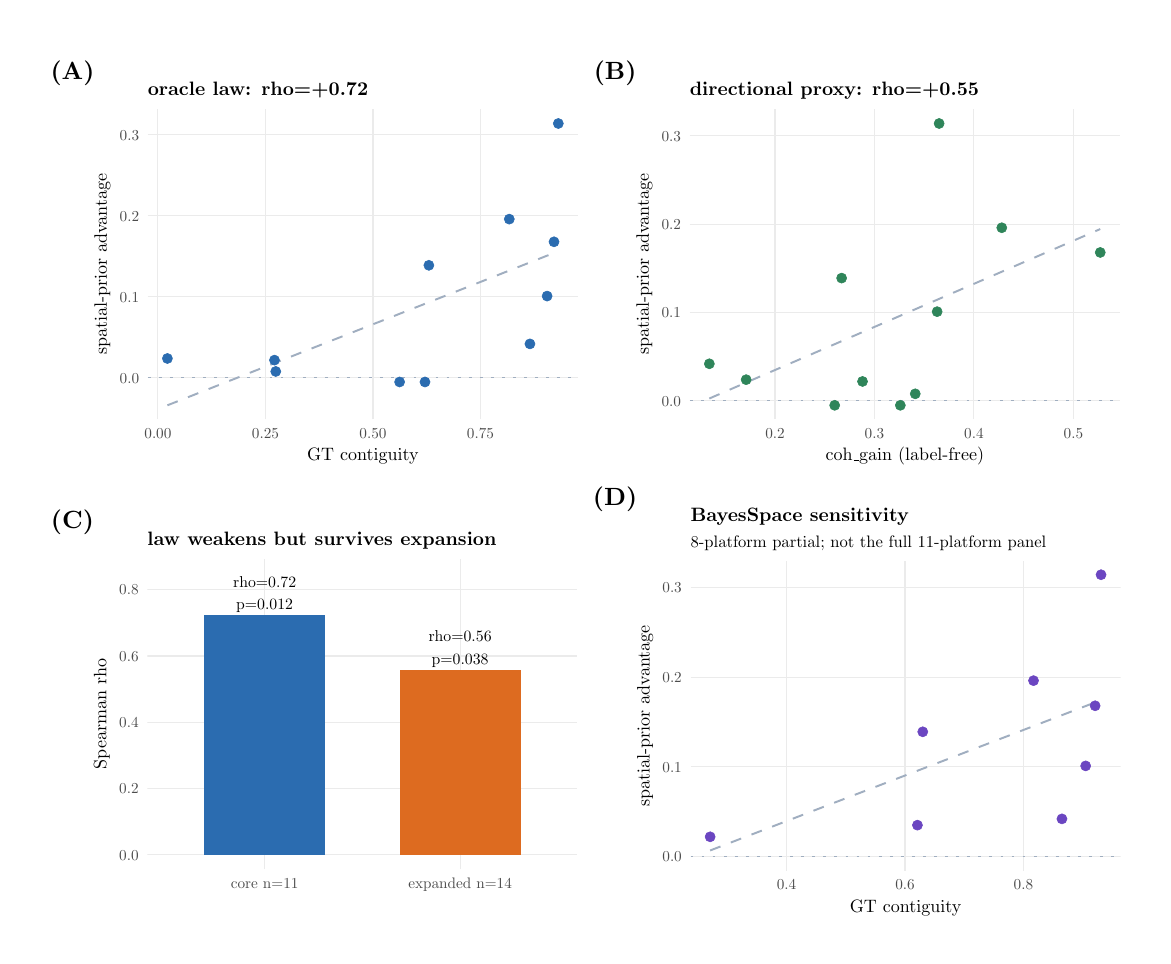
\begin{tikzpicture}[x=1pt,y=1pt]
\definecolor{fillColor}{RGB}{255,255,255}
\path[use as bounding box,fill=fillColor,fill opacity=0.00] (0,0) rectangle (403.13,328.16);
\begin{scope}
\path[clip] (  0.00,  0.00) rectangle (403.13,328.16);
\definecolor{drawColor}{RGB}{255,255,255}
\definecolor{fillColor}{RGB}{255,255,255}

\path[draw=drawColor,line width= 0.6pt,line join=round,line cap=round,fill=fillColor] (  0.00,  0.00) rectangle (403.13,328.16);
\end{scope}
\begin{scope}
\path[clip] (  5.50,164.08) rectangle (201.56,322.66);
\definecolor{drawColor}{RGB}{255,255,255}
\definecolor{fillColor}{RGB}{255,255,255}

\path[draw=drawColor,line width= 0.6pt,line join=round,line cap=round,fill=fillColor] (  5.50,164.08) rectangle (201.56,322.66);
\end{scope}
\begin{scope}
\path[clip] (201.56,164.08) rectangle (397.63,322.66);
\definecolor{drawColor}{RGB}{255,255,255}
\definecolor{fillColor}{RGB}{255,255,255}

\path[draw=drawColor,line width= 0.6pt,line join=round,line cap=round,fill=fillColor] (201.56,164.08) rectangle (397.63,322.66);
\end{scope}
\begin{scope}
\path[clip] (  4.26,167.04) rectangle (202.80,319.70);
\definecolor{fillColor}{RGB}{255,255,255}

\path[fill=fillColor] (  4.26,167.04) rectangle (202.80,319.70);
\end{scope}
\begin{scope}
\path[clip] ( 43.42,186.61) rectangle (198.80,298.63);
\definecolor{drawColor}{gray}{0.92}

\path[draw=drawColor,line width= 0.4pt,line join=round] ( 43.42,201.59) --
	(198.80,201.59);

\path[draw=drawColor,line width= 0.4pt,line join=round] ( 43.42,230.87) --
	(198.80,230.87);

\path[draw=drawColor,line width= 0.4pt,line join=round] ( 43.42,260.15) --
	(198.80,260.15);

\path[draw=drawColor,line width= 0.4pt,line join=round] ( 43.42,289.43) --
	(198.80,289.43);

\path[draw=drawColor,line width= 0.4pt,line join=round] ( 47.07,186.61) --
	( 47.07,298.63);

\path[draw=drawColor,line width= 0.4pt,line join=round] ( 85.92,186.61) --
	( 85.92,298.63);

\path[draw=drawColor,line width= 0.4pt,line join=round] (124.77,186.61) --
	(124.77,298.63);

\path[draw=drawColor,line width= 0.4pt,line join=round] (163.61,186.61) --
	(163.61,298.63);
\definecolor{drawColor}{RGB}{160,174,192}

\path[draw=drawColor,line width= 0.4pt,dash pattern=on 1pt off 3pt ,line join=round] ( 43.42,201.59) -- (198.80,201.59);

\path[draw=drawColor,line width= 0.7pt,dash pattern=on 4pt off 4pt ,line join=round] ( 50.49,191.70) --
	( 52.27,192.40) --
	( 54.06,193.11) --
	( 55.85,193.81) --
	( 57.64,194.52) --
	( 59.43,195.22) --
	( 61.21,195.93) --
	( 63.00,196.63) --
	( 64.79,197.34) --
	( 66.58,198.04) --
	( 68.37,198.75) --
	( 70.15,199.45) --
	( 71.94,200.16) --
	( 73.73,200.86) --
	( 75.52,201.56) --
	( 77.31,202.27) --
	( 79.09,202.97) --
	( 80.88,203.68) --
	( 82.67,204.38) --
	( 84.46,205.09) --
	( 86.25,205.79) --
	( 88.04,206.50) --
	( 89.82,207.20) --
	( 91.61,207.91) --
	( 93.40,208.61) --
	( 95.19,209.32) --
	( 96.98,210.02) --
	( 98.76,210.73) --
	(100.55,211.43) --
	(102.34,212.13) --
	(104.13,212.84) --
	(105.92,213.54) --
	(107.70,214.25) --
	(109.49,214.95) --
	(111.28,215.66) --
	(113.07,216.36) --
	(114.86,217.07) --
	(116.64,217.77) --
	(118.43,218.48) --
	(120.22,219.18) --
	(122.01,219.89) --
	(123.80,220.59) --
	(125.58,221.30) --
	(127.37,222.00) --
	(129.16,222.71) --
	(130.95,223.41) --
	(132.74,224.11) --
	(134.52,224.82) --
	(136.31,225.52) --
	(138.10,226.23) --
	(139.89,226.93) --
	(141.68,227.64) --
	(143.46,228.34) --
	(145.25,229.05) --
	(147.04,229.75) --
	(148.83,230.46) --
	(150.62,231.16) --
	(152.40,231.87) --
	(154.19,232.57) --
	(155.98,233.28) --
	(157.77,233.98) --
	(159.56,234.69) --
	(161.34,235.39) --
	(163.13,236.09) --
	(164.92,236.80) --
	(166.71,237.50) --
	(168.50,238.21) --
	(170.28,238.91) --
	(172.07,239.62) --
	(173.86,240.32) --
	(175.65,241.03) --
	(177.44,241.73) --
	(179.23,242.44) --
	(181.01,243.14) --
	(182.80,243.85) --
	(184.59,244.55) --
	(186.38,245.26) --
	(188.17,245.96) --
	(189.95,246.66) --
	(191.74,247.37);
\definecolor{drawColor}{RGB}{43,108,176}
\definecolor{fillColor}{RGB}{43,108,176}

\path[draw=drawColor,line width= 0.2pt,line join=round,line cap=round,fill=fillColor] (187.70,231.17) circle (  1.83);

\path[draw=drawColor,line width= 0.2pt,line join=round,line cap=round,fill=fillColor] (143.57,200.13) circle (  1.83);

\path[draw=drawColor,line width= 0.2pt,line join=round,line cap=round,fill=fillColor] (191.74,293.53) circle (  1.83);

\path[draw=drawColor,line width= 0.2pt,line join=round,line cap=round,fill=fillColor] (190.19,250.78) circle (  1.83);

\path[draw=drawColor,line width= 0.2pt,line join=round,line cap=round,fill=fillColor] (174.03,258.98) circle (  1.83);

\path[draw=drawColor,line width= 0.2pt,line join=round,line cap=round,fill=fillColor] ( 89.18,208.03) circle (  1.83);

\path[draw=drawColor,line width= 0.2pt,line join=round,line cap=round,fill=fillColor] (181.49,213.89) circle (  1.83);

\path[draw=drawColor,line width= 0.2pt,line join=round,line cap=round,fill=fillColor] (144.97,242.29) circle (  1.83);

\path[draw=drawColor,line width= 0.2pt,line join=round,line cap=round,fill=fillColor] (134.40,200.13) circle (  1.83);

\path[draw=drawColor,line width= 0.2pt,line join=round,line cap=round,fill=fillColor] ( 89.65,203.93) circle (  1.83);

\path[draw=drawColor,line width= 0.2pt,line join=round,line cap=round,fill=fillColor] ( 50.49,208.62) circle (  1.83);
\end{scope}
\begin{scope}
\path[clip] (  0.00,  0.00) rectangle (403.13,328.16);
\definecolor{drawColor}{gray}{0.30}

\node[text=drawColor,anchor=base east,inner sep=0pt, outer sep=0pt, scale=  0.55] at ( 40.27,199.70) {0.0};

\node[text=drawColor,anchor=base east,inner sep=0pt, outer sep=0pt, scale=  0.55] at ( 40.27,228.98) {0.1};

\node[text=drawColor,anchor=base east,inner sep=0pt, outer sep=0pt, scale=  0.55] at ( 40.27,258.26) {0.2};

\node[text=drawColor,anchor=base east,inner sep=0pt, outer sep=0pt, scale=  0.55] at ( 40.27,287.54) {0.3};
\end{scope}
\begin{scope}
\path[clip] (  0.00,  0.00) rectangle (403.13,328.16);
\definecolor{drawColor}{gray}{0.30}

\node[text=drawColor,anchor=base,inner sep=0pt, outer sep=0pt, scale=  0.55] at ( 47.07,179.67) {0.00};

\node[text=drawColor,anchor=base,inner sep=0pt, outer sep=0pt, scale=  0.55] at ( 85.92,179.67) {0.25};

\node[text=drawColor,anchor=base,inner sep=0pt, outer sep=0pt, scale=  0.55] at (124.77,179.67) {0.50};

\node[text=drawColor,anchor=base,inner sep=0pt, outer sep=0pt, scale=  0.55] at (163.61,179.67) {0.75};
\end{scope}
\begin{scope}
\path[clip] (  0.00,  0.00) rectangle (403.13,328.16);
\definecolor{drawColor}{RGB}{0,0,0}

\node[text=drawColor,anchor=base,inner sep=0pt, outer sep=0pt, scale=  0.65] at (121.11,171.58) {GT contiguity};
\end{scope}
\begin{scope}
\path[clip] (  0.00,  0.00) rectangle (403.13,328.16);
\definecolor{drawColor}{RGB}{0,0,0}

\node[text=drawColor,rotate= 90.00,anchor=base,inner sep=0pt, outer sep=0pt, scale=  0.65] at ( 28.61,242.62) {spatial-prior advantage};
\end{scope}
\begin{scope}
\path[clip] (  0.00,  0.00) rectangle (403.13,328.16);
\definecolor{drawColor}{RGB}{0,0,0}

\node[text=drawColor,anchor=base west,inner sep=0pt, outer sep=0pt, scale=  0.70] at ( 43.42,303.67) {\bfseries oracle law: rho=+0.72};
\end{scope}
\begin{scope}
\path[clip] (  0.00,  0.00) rectangle (403.13,328.16);
\definecolor{drawColor}{RGB}{0,0,0}

\node[text=drawColor,anchor=base,inner sep=0pt, outer sep=0pt, scale=  0.90] at ( 16.19,309.50) {\bfseries (A)};
\end{scope}
\begin{scope}
\path[clip] (200.55,167.04) rectangle (398.64,319.70);
\definecolor{fillColor}{RGB}{255,255,255}

\path[fill=fillColor] (200.55,167.04) rectangle (398.64,319.70);
\end{scope}
\begin{scope}
\path[clip] (239.26,186.61) rectangle (394.64,298.63);
\definecolor{drawColor}{gray}{0.92}

\path[draw=drawColor,line width= 0.4pt,line join=round] (239.26,193.29) --
	(394.64,193.29);

\path[draw=drawColor,line width= 0.4pt,line join=round] (239.26,225.22) --
	(394.64,225.22);

\path[draw=drawColor,line width= 0.4pt,line join=round] (239.26,257.14) --
	(394.64,257.14);

\path[draw=drawColor,line width= 0.4pt,line join=round] (239.26,289.06) --
	(394.64,289.06);

\path[draw=drawColor,line width= 0.4pt,line join=round] (270.04,186.61) --
	(270.04,298.63);

\path[draw=drawColor,line width= 0.4pt,line join=round] (305.98,186.61) --
	(305.98,298.63);

\path[draw=drawColor,line width= 0.4pt,line join=round] (341.93,186.61) --
	(341.93,298.63);

\path[draw=drawColor,line width= 0.4pt,line join=round] (377.87,186.61) --
	(377.87,298.63);
\definecolor{drawColor}{RGB}{160,174,192}

\path[draw=drawColor,line width= 0.4pt,dash pattern=on 1pt off 3pt ,line join=round] (239.26,193.29) -- (394.64,193.29);

\path[draw=drawColor,line width= 0.7pt,dash pattern=on 4pt off 4pt ,line join=round] (246.32,194.16) --
	(248.11,194.94) --
	(249.89,195.71) --
	(251.68,196.49) --
	(253.47,197.26) --
	(255.26,198.04) --
	(257.05,198.81) --
	(258.83,199.59) --
	(260.62,200.36) --
	(262.41,201.14) --
	(264.20,201.91) --
	(265.99,202.69) --
	(267.77,203.46) --
	(269.56,204.24) --
	(271.35,205.01) --
	(273.14,205.79) --
	(274.93,206.56) --
	(276.71,207.34) --
	(278.50,208.11) --
	(280.29,208.89) --
	(282.08,209.66) --
	(283.87,210.44) --
	(285.65,211.21) --
	(287.44,211.99) --
	(289.23,212.76) --
	(291.02,213.54) --
	(292.81,214.31) --
	(294.59,215.09) --
	(296.38,215.86) --
	(298.17,216.64) --
	(299.96,217.41) --
	(301.75,218.19) --
	(303.54,218.96) --
	(305.32,219.74) --
	(307.11,220.51) --
	(308.90,221.29) --
	(310.69,222.06) --
	(312.48,222.84) --
	(314.26,223.61) --
	(316.05,224.39) --
	(317.84,225.16) --
	(319.63,225.94) --
	(321.42,226.71) --
	(323.20,227.49) --
	(324.99,228.26) --
	(326.78,229.04) --
	(328.57,229.81) --
	(330.36,230.59) --
	(332.14,231.36) --
	(333.93,232.14) --
	(335.72,232.91) --
	(337.51,233.69) --
	(339.30,234.46) --
	(341.08,235.24) --
	(342.87,236.01) --
	(344.66,236.79) --
	(346.45,237.56) --
	(348.24,238.34) --
	(350.02,239.11) --
	(351.81,239.89) --
	(353.60,240.66) --
	(355.39,241.44) --
	(357.18,242.21) --
	(358.96,242.99) --
	(360.75,243.76) --
	(362.54,244.54) --
	(364.33,245.31) --
	(366.12,246.09) --
	(367.90,246.86) --
	(369.69,247.64) --
	(371.48,248.41) --
	(373.27,249.19) --
	(375.06,249.96) --
	(376.84,250.74) --
	(378.63,251.51) --
	(380.42,252.29) --
	(382.21,253.06) --
	(384.00,253.84) --
	(385.78,254.61) --
	(387.57,255.39);
\definecolor{drawColor}{RGB}{47,133,90}
\definecolor{fillColor}{RGB}{47,133,90}

\path[draw=drawColor,line width= 0.2pt,line join=round,line cap=round,fill=fillColor] (328.63,225.54) circle (  1.83);

\path[draw=drawColor,line width= 0.2pt,line join=round,line cap=round,fill=fillColor] (315.33,191.70) circle (  1.83);

\path[draw=drawColor,line width= 0.2pt,line join=round,line cap=round,fill=fillColor] (329.35,293.53) circle (  1.83);

\path[draw=drawColor,line width= 0.2pt,line join=round,line cap=round,fill=fillColor] (387.57,246.93) circle (  1.83);

\path[draw=drawColor,line width= 0.2pt,line join=round,line cap=round,fill=fillColor] (351.99,255.86) circle (  1.83);

\path[draw=drawColor,line width= 0.2pt,line join=round,line cap=round,fill=fillColor] (301.67,200.32) circle (  1.83);

\path[draw=drawColor,line width= 0.2pt,line join=round,line cap=round,fill=fillColor] (246.32,206.70) circle (  1.83);

\path[draw=drawColor,line width= 0.2pt,line join=round,line cap=round,fill=fillColor] (294.12,237.67) circle (  1.83);

\path[draw=drawColor,line width= 0.2pt,line join=round,line cap=round,fill=fillColor] (291.61,191.70) circle (  1.83);

\path[draw=drawColor,line width= 0.2pt,line join=round,line cap=round,fill=fillColor] (320.72,195.85) circle (  1.83);

\path[draw=drawColor,line width= 0.2pt,line join=round,line cap=round,fill=fillColor] (259.62,200.96) circle (  1.83);
\end{scope}
\begin{scope}
\path[clip] (  0.00,  0.00) rectangle (403.13,328.16);
\definecolor{drawColor}{gray}{0.30}

\node[text=drawColor,anchor=base east,inner sep=0pt, outer sep=0pt, scale=  0.55] at (236.11,191.40) {0.0};

\node[text=drawColor,anchor=base east,inner sep=0pt, outer sep=0pt, scale=  0.55] at (236.11,223.32) {0.1};

\node[text=drawColor,anchor=base east,inner sep=0pt, outer sep=0pt, scale=  0.55] at (236.11,255.25) {0.2};

\node[text=drawColor,anchor=base east,inner sep=0pt, outer sep=0pt, scale=  0.55] at (236.11,287.17) {0.3};
\end{scope}
\begin{scope}
\path[clip] (  0.00,  0.00) rectangle (403.13,328.16);
\definecolor{drawColor}{gray}{0.30}

\node[text=drawColor,anchor=base,inner sep=0pt, outer sep=0pt, scale=  0.55] at (270.04,179.67) {0.2};

\node[text=drawColor,anchor=base,inner sep=0pt, outer sep=0pt, scale=  0.55] at (305.98,179.67) {0.3};

\node[text=drawColor,anchor=base,inner sep=0pt, outer sep=0pt, scale=  0.55] at (341.93,179.67) {0.4};

\node[text=drawColor,anchor=base,inner sep=0pt, outer sep=0pt, scale=  0.55] at (377.87,179.67) {0.5};
\end{scope}
\begin{scope}
\path[clip] (  0.00,  0.00) rectangle (403.13,328.16);
\definecolor{drawColor}{RGB}{0,0,0}

\node[text=drawColor,anchor=base,inner sep=0pt, outer sep=0pt, scale=  0.65] at (316.95,171.58) {coh{\_{}}gain (label-free)};
\end{scope}
\begin{scope}
\path[clip] (  0.00,  0.00) rectangle (403.13,328.16);
\definecolor{drawColor}{RGB}{0,0,0}

\node[text=drawColor,rotate= 90.00,anchor=base,inner sep=0pt, outer sep=0pt, scale=  0.65] at (224.44,242.62) {spatial-prior advantage};
\end{scope}
\begin{scope}
\path[clip] (  0.00,  0.00) rectangle (403.13,328.16);
\definecolor{drawColor}{RGB}{0,0,0}

\node[text=drawColor,anchor=base west,inner sep=0pt, outer sep=0pt, scale=  0.70] at (239.26,303.67) {\bfseries directional proxy: rho=+0.55};
\end{scope}
\begin{scope}
\path[clip] (  0.00,  0.00) rectangle (403.13,328.16);
\definecolor{drawColor}{RGB}{0,0,0}

\node[text=drawColor,anchor=base,inner sep=0pt, outer sep=0pt, scale=  0.90] at (212.26,309.50) {\bfseries (B)};
\end{scope}
\begin{scope}
\path[clip] (  5.50,  5.50) rectangle (201.56,164.08);
\definecolor{drawColor}{RGB}{255,255,255}
\definecolor{fillColor}{RGB}{255,255,255}

\path[draw=drawColor,line width= 0.6pt,line join=round,line cap=round,fill=fillColor] (  5.50,  5.50) rectangle (201.56,164.08);
\end{scope}
\begin{scope}
\path[clip] (201.56,  5.50) rectangle (397.63,164.08);
\definecolor{drawColor}{RGB}{255,255,255}
\definecolor{fillColor}{RGB}{255,255,255}

\path[draw=drawColor,line width= 0.6pt,line join=round,line cap=round,fill=fillColor] (201.56,  5.50) rectangle (397.63,164.08);
\end{scope}
\begin{scope}
\path[clip] (  4.43, 12.34) rectangle (202.63,157.24);
\definecolor{fillColor}{RGB}{255,255,255}

\path[fill=fillColor] (  4.43, 12.34) rectangle (202.63,157.24);
\end{scope}
\begin{scope}
\path[clip] ( 43.25, 24.14) rectangle (198.63,136.16);
\definecolor{drawColor}{gray}{0.92}

\path[draw=drawColor,line width= 0.4pt,line join=round] ( 43.25, 29.23) --
	(198.63, 29.23);

\path[draw=drawColor,line width= 0.4pt,line join=round] ( 43.25, 53.20) --
	(198.63, 53.20);

\path[draw=drawColor,line width= 0.4pt,line join=round] ( 43.25, 77.16) --
	(198.63, 77.16);

\path[draw=drawColor,line width= 0.4pt,line join=round] ( 43.25,101.12) --
	(198.63,101.12);

\path[draw=drawColor,line width= 0.4pt,line join=round] ( 43.25,125.08) --
	(198.63,125.08);

\path[draw=drawColor,line width= 0.4pt,line join=round] ( 85.63, 24.14) --
	( 85.63,136.16);

\path[draw=drawColor,line width= 0.4pt,line join=round] (156.25, 24.14) --
	(156.25,136.16);
\definecolor{fillColor}{RGB}{43,108,176}

\path[fill=fillColor] ( 63.73, 29.23) rectangle (107.52,115.97);
\definecolor{fillColor}{RGB}{221,107,32}

\path[fill=fillColor] (134.36, 29.23) rectangle (178.15, 96.21);
\definecolor{drawColor}{RGB}{0,0,0}

\node[text=drawColor,anchor=base,inner sep=0pt, outer sep=0pt, scale=  0.57] at ( 85.63,125.98) {rho=0.72};

\node[text=drawColor,anchor=base,inner sep=0pt, outer sep=0pt, scale=  0.57] at ( 85.63,117.79) {p=0.012};

\node[text=drawColor,anchor=base,inner sep=0pt, outer sep=0pt, scale=  0.57] at (156.25,106.22) {rho=0.56};

\node[text=drawColor,anchor=base,inner sep=0pt, outer sep=0pt, scale=  0.57] at (156.25, 98.02) {p=0.038};
\end{scope}
\begin{scope}
\path[clip] (  0.00,  0.00) rectangle (403.13,328.16);
\definecolor{drawColor}{gray}{0.30}

\node[text=drawColor,anchor=base east,inner sep=0pt, outer sep=0pt, scale=  0.55] at ( 40.10, 27.34) {0.0};

\node[text=drawColor,anchor=base east,inner sep=0pt, outer sep=0pt, scale=  0.55] at ( 40.10, 51.30) {0.2};

\node[text=drawColor,anchor=base east,inner sep=0pt, outer sep=0pt, scale=  0.55] at ( 40.10, 75.26) {0.4};

\node[text=drawColor,anchor=base east,inner sep=0pt, outer sep=0pt, scale=  0.55] at ( 40.10, 99.22) {0.6};

\node[text=drawColor,anchor=base east,inner sep=0pt, outer sep=0pt, scale=  0.55] at ( 40.10,123.18) {0.8};
\end{scope}
\begin{scope}
\path[clip] (  0.00,  0.00) rectangle (403.13,328.16);
\definecolor{drawColor}{gray}{0.30}

\node[text=drawColor,anchor=base,inner sep=0pt, outer sep=0pt, scale=  0.55] at ( 85.63, 17.20) {core n=11};

\node[text=drawColor,anchor=base,inner sep=0pt, outer sep=0pt, scale=  0.55] at (156.25, 17.20) {expanded n=14};
\end{scope}
\begin{scope}
\path[clip] (  0.00,  0.00) rectangle (403.13,328.16);
\definecolor{drawColor}{RGB}{0,0,0}

\node[text=drawColor,rotate= 90.00,anchor=base,inner sep=0pt, outer sep=0pt, scale=  0.65] at ( 28.43, 80.15) {Spearman rho};
\end{scope}
\begin{scope}
\path[clip] (  0.00,  0.00) rectangle (403.13,328.16);
\definecolor{drawColor}{RGB}{0,0,0}

\node[text=drawColor,anchor=base west,inner sep=0pt, outer sep=0pt, scale=  0.70] at ( 43.25,141.21) {\bfseries law weakens but survives expansion};
\end{scope}
\begin{scope}
\path[clip] (  0.00,  0.00) rectangle (403.13,328.16);
\definecolor{drawColor}{RGB}{0,0,0}

\node[text=drawColor,anchor=base,inner sep=0pt, outer sep=0pt, scale=  0.90] at ( 16.19,147.03) {\bfseries (C)};
\end{scope}
\begin{scope}
\path[clip] (200.27,  3.98) rectangle (398.92,165.60);
\definecolor{fillColor}{RGB}{255,255,255}

\path[fill=fillColor] (200.27,  3.98) rectangle (398.92,165.60);
\end{scope}
\begin{scope}
\path[clip] (239.54, 23.55) rectangle (394.92,135.57);
\definecolor{drawColor}{gray}{0.92}

\path[draw=drawColor,line width= 0.4pt,line join=round] (239.54, 28.64) --
	(394.92, 28.64);

\path[draw=drawColor,line width= 0.4pt,line join=round] (239.54, 61.07) --
	(394.92, 61.07);

\path[draw=drawColor,line width= 0.4pt,line join=round] (239.54, 93.50) --
	(394.92, 93.50);

\path[draw=drawColor,line width= 0.4pt,line join=round] (239.54,125.94) --
	(394.92,125.94);

\path[draw=drawColor,line width= 0.4pt,line join=round] (274.21, 23.55) --
	(274.21,135.57);

\path[draw=drawColor,line width= 0.4pt,line join=round] (317.02, 23.55) --
	(317.02,135.57);

\path[draw=drawColor,line width= 0.4pt,line join=round] (359.82, 23.55) --
	(359.82,135.57);
\definecolor{drawColor}{RGB}{160,174,192}

\path[draw=drawColor,line width= 0.4pt,dash pattern=on 1pt off 3pt ,line join=round] (239.54, 28.64) -- (394.92, 28.64);

\path[draw=drawColor,line width= 0.7pt,dash pattern=on 4pt off 4pt ,line join=round] (246.61, 30.84) --
	(248.39, 31.53) --
	(250.18, 32.21) --
	(251.97, 32.90) --
	(253.76, 33.59) --
	(255.55, 34.28) --
	(257.33, 34.97) --
	(259.12, 35.65) --
	(260.91, 36.34) --
	(262.70, 37.03) --
	(264.49, 37.72) --
	(266.27, 38.40) --
	(268.06, 39.09) --
	(269.85, 39.78) --
	(271.64, 40.47) --
	(273.43, 41.16) --
	(275.21, 41.84) --
	(277.00, 42.53) --
	(278.79, 43.22) --
	(280.58, 43.91) --
	(282.37, 44.59) --
	(284.15, 45.28) --
	(285.94, 45.97) --
	(287.73, 46.66) --
	(289.52, 47.35) --
	(291.31, 48.03) --
	(293.09, 48.72) --
	(294.88, 49.41) --
	(296.67, 50.10) --
	(298.46, 50.78) --
	(300.25, 51.47) --
	(302.03, 52.16) --
	(303.82, 52.85) --
	(305.61, 53.53) --
	(307.40, 54.22) --
	(309.19, 54.91) --
	(310.97, 55.60) --
	(312.76, 56.29) --
	(314.55, 56.97) --
	(316.34, 57.66) --
	(318.13, 58.35) --
	(319.91, 59.04) --
	(321.70, 59.72) --
	(323.49, 60.41) --
	(325.28, 61.10) --
	(327.07, 61.79) --
	(328.86, 62.48) --
	(330.64, 63.16) --
	(332.43, 63.85) --
	(334.22, 64.54) --
	(336.01, 65.23) --
	(337.80, 65.91) --
	(339.58, 66.60) --
	(341.37, 67.29) --
	(343.16, 67.98) --
	(344.95, 68.67) --
	(346.74, 69.35) --
	(348.52, 70.04) --
	(350.31, 70.73) --
	(352.10, 71.42) --
	(353.89, 72.10) --
	(355.68, 72.79) --
	(357.46, 73.48) --
	(359.25, 74.17) --
	(361.04, 74.86) --
	(362.83, 75.54) --
	(364.62, 76.23) --
	(366.40, 76.92) --
	(368.19, 77.61) --
	(369.98, 78.29) --
	(371.77, 78.98) --
	(373.56, 79.67) --
	(375.34, 80.36) --
	(377.13, 81.05) --
	(378.92, 81.73) --
	(380.71, 82.42) --
	(382.50, 83.11) --
	(384.28, 83.80) --
	(386.07, 84.48) --
	(387.86, 85.17);
\definecolor{drawColor}{RGB}{107,70,193}
\definecolor{fillColor}{RGB}{107,70,193}

\path[draw=drawColor,line width= 0.2pt,line join=round,line cap=round,fill=fillColor] (382.30, 61.40) circle (  1.83);

\path[draw=drawColor,line width= 0.2pt,line join=round,line cap=round,fill=fillColor] (373.73, 42.26) circle (  1.83);

\path[draw=drawColor,line width= 0.2pt,line join=round,line cap=round,fill=fillColor] (321.51, 39.99) circle (  1.83);

\path[draw=drawColor,line width= 0.2pt,line join=round,line cap=round,fill=fillColor] (387.86,130.48) circle (  1.83);

\path[draw=drawColor,line width= 0.2pt,line join=round,line cap=round,fill=fillColor] (385.72, 83.13) circle (  1.83);

\path[draw=drawColor,line width= 0.2pt,line join=round,line cap=round,fill=fillColor] (363.46, 92.21) circle (  1.83);

\path[draw=drawColor,line width= 0.2pt,line join=round,line cap=round,fill=fillColor] (246.61, 35.78) circle (  1.83);

\path[draw=drawColor,line width= 0.2pt,line join=round,line cap=round,fill=fillColor] (323.44, 73.72) circle (  1.83);
\end{scope}
\begin{scope}
\path[clip] (  0.00,  0.00) rectangle (403.13,328.16);
\definecolor{drawColor}{gray}{0.30}

\node[text=drawColor,anchor=base east,inner sep=0pt, outer sep=0pt, scale=  0.55] at (236.39, 26.75) {0.0};

\node[text=drawColor,anchor=base east,inner sep=0pt, outer sep=0pt, scale=  0.55] at (236.39, 59.18) {0.1};

\node[text=drawColor,anchor=base east,inner sep=0pt, outer sep=0pt, scale=  0.55] at (236.39, 91.61) {0.2};

\node[text=drawColor,anchor=base east,inner sep=0pt, outer sep=0pt, scale=  0.55] at (236.39,124.04) {0.3};
\end{scope}
\begin{scope}
\path[clip] (  0.00,  0.00) rectangle (403.13,328.16);
\definecolor{drawColor}{gray}{0.30}

\node[text=drawColor,anchor=base,inner sep=0pt, outer sep=0pt, scale=  0.55] at (274.21, 16.61) {0.4};

\node[text=drawColor,anchor=base,inner sep=0pt, outer sep=0pt, scale=  0.55] at (317.02, 16.61) {0.6};

\node[text=drawColor,anchor=base,inner sep=0pt, outer sep=0pt, scale=  0.55] at (359.82, 16.61) {0.8};
\end{scope}
\begin{scope}
\path[clip] (  0.00,  0.00) rectangle (403.13,328.16);
\definecolor{drawColor}{RGB}{0,0,0}

\node[text=drawColor,anchor=base,inner sep=0pt, outer sep=0pt, scale=  0.65] at (317.23,  8.52) {GT contiguity};
\end{scope}
\begin{scope}
\path[clip] (  0.00,  0.00) rectangle (403.13,328.16);
\definecolor{drawColor}{RGB}{0,0,0}

\node[text=drawColor,rotate= 90.00,anchor=base,inner sep=0pt, outer sep=0pt, scale=  0.65] at (224.73, 79.56) {spatial-prior advantage};
\end{scope}
\begin{scope}
\path[clip] (  0.00,  0.00) rectangle (403.13,328.16);
\definecolor{drawColor}{RGB}{0,0,0}

\node[text=drawColor,anchor=base west,inner sep=0pt, outer sep=0pt, scale=  0.60] at (239.54,140.39) {8-platform partial; not the full 11-platform panel};
\end{scope}
\begin{scope}
\path[clip] (  0.00,  0.00) rectangle (403.13,328.16);
\definecolor{drawColor}{RGB}{0,0,0}

\node[text=drawColor,anchor=base west,inner sep=0pt, outer sep=0pt, scale=  0.70] at (239.54,149.57) {\bfseries BayesSpace sensitivity};
\end{scope}
\begin{scope}
\path[clip] (  0.00,  0.00) rectangle (403.13,328.16);
\definecolor{drawColor}{RGB}{0,0,0}

\node[text=drawColor,anchor=base,inner sep=0pt, outer sep=0pt, scale=  0.90] at (212.26,155.40) {\bfseries (D)};
\end{scope}
\end{tikzpicture}
}
\caption{(a) The headline law: spatial-prior advantage versus GT spatial contiguity (oracle), $\rho=+0.72$.
(b) The same trend recovered by the label-free \texttt{coh\_gain} proxy, $\rho=+0.55$, the rule applied
without labels.}
\label{fig:law}
\end{figure}

\begin{figure}[htbp]\centering
\resizebox{\linewidth}{!}{% !TEX encoding = UTF-8 Unicode
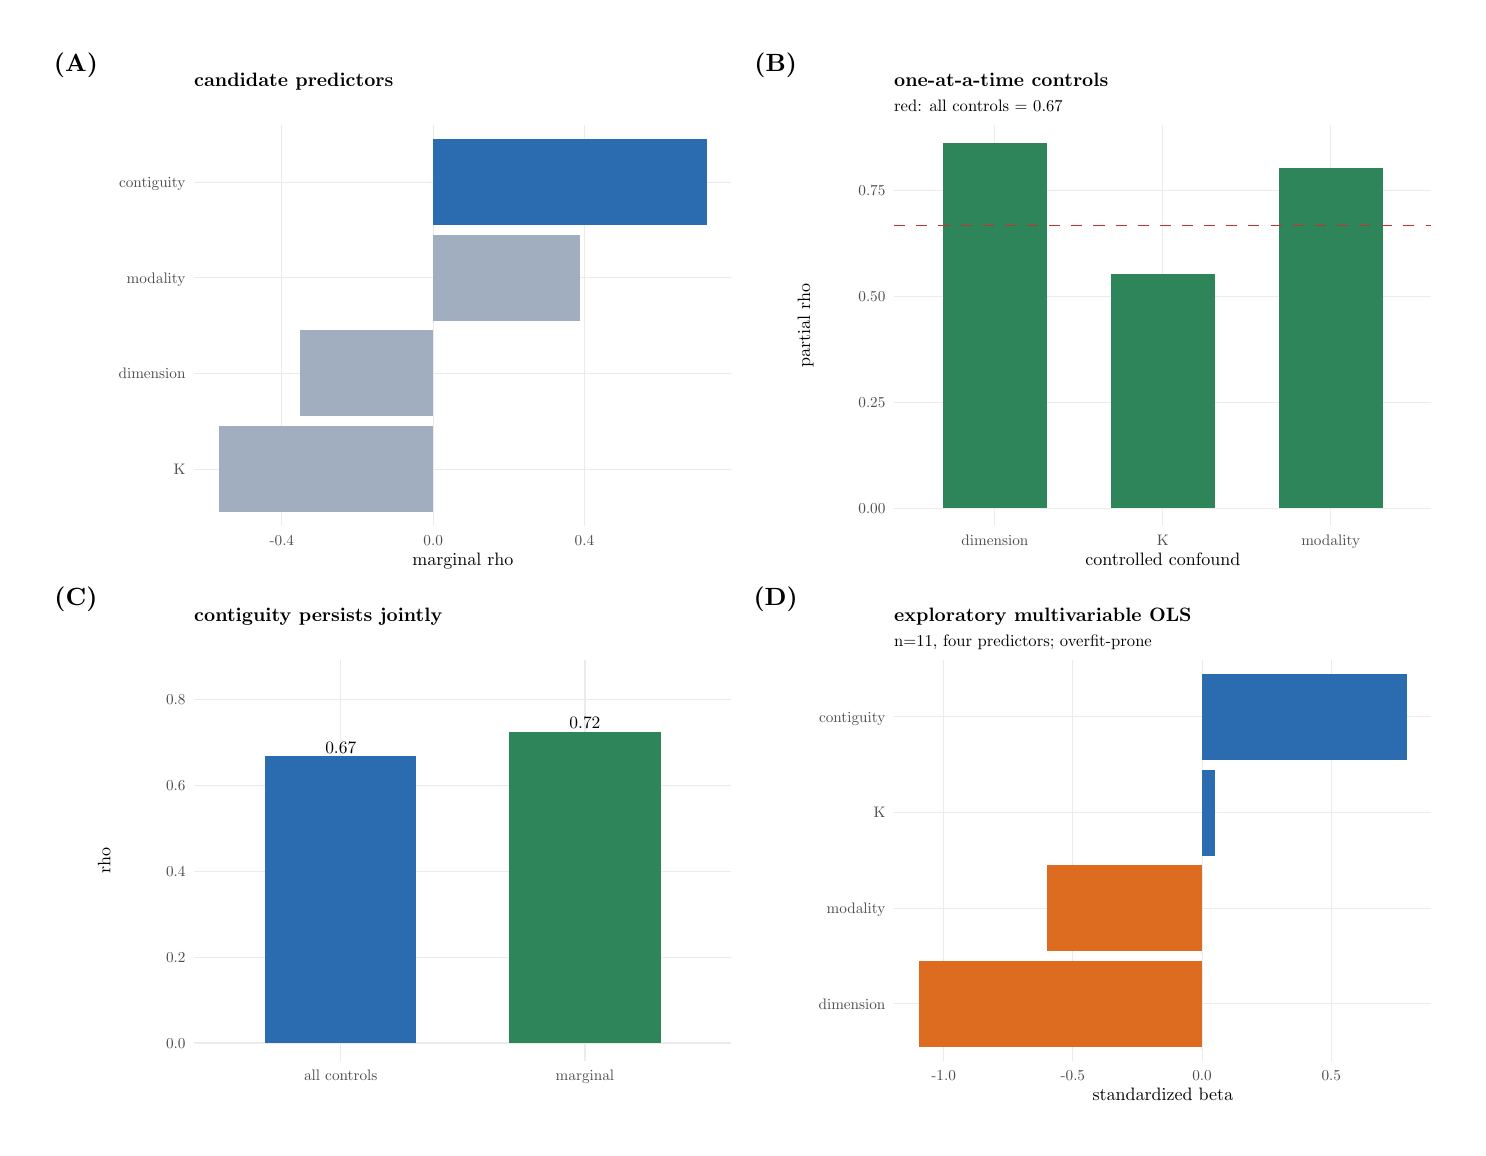
\begin{tikzpicture}[x=1pt,y=1pt]
\definecolor{fillColor}{RGB}{255,255,255}
\path[use as bounding box,fill=fillColor,fill opacity=0.00] (0,0) rectangle (516.73,397.48);
\begin{scope}
\path[clip] (  0.00,  0.00) rectangle (516.73,397.48);
\definecolor{drawColor}{RGB}{255,255,255}
\definecolor{fillColor}{RGB}{255,255,255}

\path[draw=drawColor,line width= 0.6pt,line join=round,line cap=round,fill=fillColor] (  0.00,  0.00) rectangle (516.73,397.48);
\end{scope}
\begin{scope}
\path[clip] (  5.50,198.74) rectangle (258.31,391.98);
\definecolor{fillColor}{RGB}{255,255,255}

\path[fill=fillColor] (  5.50,198.74) rectangle (258.31,391.98);
\end{scope}
\begin{scope}
\path[clip] (258.31,198.74) rectangle (511.23,391.98);
\definecolor{fillColor}{RGB}{255,255,255}

\path[fill=fillColor] (258.31,198.74) rectangle (511.23,391.98);
\end{scope}
\begin{scope}
\path[clip] (  5.50,  5.50) rectangle (258.31,198.74);
\definecolor{fillColor}{RGB}{255,255,255}

\path[fill=fillColor] (  5.50,  5.50) rectangle (258.31,198.74);
\end{scope}
\begin{scope}
\path[clip] (258.31,  5.50) rectangle (511.23,198.74);
\definecolor{fillColor}{RGB}{255,255,255}

\path[fill=fillColor] (258.31,  5.50) rectangle (511.23,198.74);
\end{scope}
\begin{scope}
\path[clip] ( 60.18,217.24) rectangle (254.31,362.39);
\definecolor{drawColor}{gray}{0.92}

\path[draw=drawColor,line width= 0.4pt,line join=round] ( 60.18,237.98) --
	(254.31,237.98);

\path[draw=drawColor,line width= 0.4pt,line join=round] ( 60.18,272.54) --
	(254.31,272.54);

\path[draw=drawColor,line width= 0.4pt,line join=round] ( 60.18,307.10) --
	(254.31,307.10);

\path[draw=drawColor,line width= 0.4pt,line join=round] ( 60.18,341.65) --
	(254.31,341.65);

\path[draw=drawColor,line width= 0.4pt,line join=round] ( 91.84,217.24) --
	( 91.84,362.39);

\path[draw=drawColor,line width= 0.4pt,line join=round] (146.52,217.24) --
	(146.52,362.39);

\path[draw=drawColor,line width= 0.4pt,line join=round] (201.20,217.24) --
	(201.20,362.39);
\definecolor{fillColor}{RGB}{43,108,176}

\path[fill=fillColor] (146.52,326.10) rectangle (245.49,357.21);
\definecolor{fillColor}{RGB}{160,174,192}

\path[fill=fillColor] ( 69.01,222.43) rectangle (146.52,253.53);

\path[fill=fillColor] ( 98.40,256.98) rectangle (146.52,288.09);

\path[fill=fillColor] (146.52,291.54) rectangle (199.69,322.65);
\end{scope}
\begin{scope}
\path[clip] (  0.00,  0.00) rectangle (516.73,397.48);
\definecolor{drawColor}{gray}{0.30}

\node[text=drawColor,anchor=base east,inner sep=0pt, outer sep=0pt, scale=  0.55] at ( 57.03,236.08) {K};

\node[text=drawColor,anchor=base east,inner sep=0pt, outer sep=0pt, scale=  0.55] at ( 57.03,270.64) {dimension};

\node[text=drawColor,anchor=base east,inner sep=0pt, outer sep=0pt, scale=  0.55] at ( 57.03,305.20) {modality};

\node[text=drawColor,anchor=base east,inner sep=0pt, outer sep=0pt, scale=  0.55] at ( 57.03,339.76) {contiguity};
\end{scope}
\begin{scope}
\path[clip] (  0.00,  0.00) rectangle (516.73,397.48);
\definecolor{drawColor}{gray}{0.30}

\node[text=drawColor,anchor=base,inner sep=0pt, outer sep=0pt, scale=  0.55] at ( 91.84,210.30) {-0.4};

\node[text=drawColor,anchor=base,inner sep=0pt, outer sep=0pt, scale=  0.55] at (146.52,210.30) {0.0};

\node[text=drawColor,anchor=base,inner sep=0pt, outer sep=0pt, scale=  0.55] at (201.20,210.30) {0.4};
\end{scope}
\begin{scope}
\path[clip] (  0.00,  0.00) rectangle (516.73,397.48);
\definecolor{drawColor}{RGB}{0,0,0}

\node[text=drawColor,anchor=base,inner sep=0pt, outer sep=0pt, scale=  0.65] at (157.25,203.01) {marginal rho};
\end{scope}
\begin{scope}
\path[clip] (  0.00,  0.00) rectangle (516.73,397.48);
\definecolor{drawColor}{RGB}{0,0,0}

\node[text=drawColor,anchor=base west,inner sep=0pt, outer sep=0pt, scale=  0.70] at ( 60.18,376.05) {\bfseries candidate predictors};
\end{scope}
\begin{scope}
\path[clip] (  0.00,  0.00) rectangle (516.73,397.48);
\definecolor{drawColor}{RGB}{0,0,0}

\node[text=drawColor,anchor=base,inner sep=0pt, outer sep=0pt, scale=  0.90] at ( 17.44,381.82) {\bfseries (A)};
\end{scope}
\begin{scope}
\path[clip] (313.11,217.24) rectangle (507.23,362.39);
\definecolor{drawColor}{gray}{0.92}

\path[draw=drawColor,line width= 0.4pt,line join=round] (313.11,223.84) --
	(507.23,223.84);

\path[draw=drawColor,line width= 0.4pt,line join=round] (313.11,262.15) --
	(507.23,262.15);

\path[draw=drawColor,line width= 0.4pt,line join=round] (313.11,300.47) --
	(507.23,300.47);

\path[draw=drawColor,line width= 0.4pt,line join=round] (313.11,338.78) --
	(507.23,338.78);

\path[draw=drawColor,line width= 0.4pt,line join=round] (349.50,217.24) --
	(349.50,362.39);

\path[draw=drawColor,line width= 0.4pt,line join=round] (410.17,217.24) --
	(410.17,362.39);

\path[draw=drawColor,line width= 0.4pt,line join=round] (470.83,217.24) --
	(470.83,362.39);
\definecolor{fillColor}{RGB}{47,133,90}

\path[fill=fillColor] (391.36,223.84) rectangle (428.97,308.44);

\path[fill=fillColor] (330.70,223.84) rectangle (368.31,355.79);

\path[fill=fillColor] (452.03,223.84) rectangle (489.64,346.60);
\definecolor{drawColor}{RGB}{197,48,48}

\path[draw=drawColor,line width= 0.4pt,dash pattern=on 4pt off 4pt ,line join=round] (313.11,326.06) -- (507.23,326.06);
\end{scope}
\begin{scope}
\path[clip] (  0.00,  0.00) rectangle (516.73,397.48);
\definecolor{drawColor}{gray}{0.30}

\node[text=drawColor,anchor=base east,inner sep=0pt, outer sep=0pt, scale=  0.55] at (309.96,221.95) {0.00};

\node[text=drawColor,anchor=base east,inner sep=0pt, outer sep=0pt, scale=  0.55] at (309.96,260.26) {0.25};

\node[text=drawColor,anchor=base east,inner sep=0pt, outer sep=0pt, scale=  0.55] at (309.96,298.57) {0.50};

\node[text=drawColor,anchor=base east,inner sep=0pt, outer sep=0pt, scale=  0.55] at (309.96,336.89) {0.75};
\end{scope}
\begin{scope}
\path[clip] (  0.00,  0.00) rectangle (516.73,397.48);
\definecolor{drawColor}{gray}{0.30}

\node[text=drawColor,anchor=base,inner sep=0pt, outer sep=0pt, scale=  0.55] at (349.50,210.30) {dimension};

\node[text=drawColor,anchor=base,inner sep=0pt, outer sep=0pt, scale=  0.55] at (410.17,210.30) {K};

\node[text=drawColor,anchor=base,inner sep=0pt, outer sep=0pt, scale=  0.55] at (470.83,210.30) {modality};
\end{scope}
\begin{scope}
\path[clip] (  0.00,  0.00) rectangle (516.73,397.48);
\definecolor{drawColor}{RGB}{0,0,0}

\node[text=drawColor,anchor=base,inner sep=0pt, outer sep=0pt, scale=  0.65] at (410.17,203.01) {controlled confound};
\end{scope}
\begin{scope}
\path[clip] (  0.00,  0.00) rectangle (516.73,397.48);
\definecolor{drawColor}{RGB}{0,0,0}

\node[text=drawColor,rotate= 90.00,anchor=base,inner sep=0pt, outer sep=0pt, scale=  0.65] at (282.77,289.82) {partial rho};
\end{scope}
\begin{scope}
\path[clip] (  0.00,  0.00) rectangle (516.73,397.48);
\definecolor{drawColor}{RGB}{0,0,0}

\node[text=drawColor,anchor=base west,inner sep=0pt, outer sep=0pt, scale=  0.60] at (313.11,367.06) {red: all controls = 0.67};
\end{scope}
\begin{scope}
\path[clip] (  0.00,  0.00) rectangle (516.73,397.48);
\definecolor{drawColor}{RGB}{0,0,0}

\node[text=drawColor,anchor=base west,inner sep=0pt, outer sep=0pt, scale=  0.70] at (313.11,376.05) {\bfseries one-at-a-time controls};
\end{scope}
\begin{scope}
\path[clip] (  0.00,  0.00) rectangle (516.73,397.48);
\definecolor{drawColor}{RGB}{0,0,0}

\node[text=drawColor,anchor=base,inner sep=0pt, outer sep=0pt, scale=  0.90] at (270.30,381.82) {\bfseries (B)};
\end{scope}
\begin{scope}
\path[clip] ( 60.18, 24.00) rectangle (254.31,169.15);
\definecolor{drawColor}{gray}{0.92}

\path[draw=drawColor,line width= 0.4pt,line join=round] ( 60.18, 30.60) --
	(254.31, 30.60);

\path[draw=drawColor,line width= 0.4pt,line join=round] ( 60.18, 61.64) --
	(254.31, 61.64);

\path[draw=drawColor,line width= 0.4pt,line join=round] ( 60.18, 92.69) --
	(254.31, 92.69);

\path[draw=drawColor,line width= 0.4pt,line join=round] ( 60.18,123.74) --
	(254.31,123.74);

\path[draw=drawColor,line width= 0.4pt,line join=round] ( 60.18,154.79) --
	(254.31,154.79);

\path[draw=drawColor,line width= 0.4pt,line join=round] (113.13, 24.00) --
	(113.13,169.15);

\path[draw=drawColor,line width= 0.4pt,line join=round] (201.37, 24.00) --
	(201.37,169.15);
\definecolor{fillColor}{RGB}{47,133,90}

\path[fill=fillColor] (174.01, 30.60) rectangle (228.72,142.99);
\definecolor{fillColor}{RGB}{43,108,176}

\path[fill=fillColor] ( 85.77, 30.60) rectangle (140.48,134.14);
\definecolor{drawColor}{RGB}{0,0,0}

\node[text=drawColor,anchor=base,inner sep=0pt, outer sep=0pt, scale=  0.63] at (201.37,144.07) {0.72};

\node[text=drawColor,anchor=base,inner sep=0pt, outer sep=0pt, scale=  0.63] at (113.13,135.22) {0.67};
\end{scope}
\begin{scope}
\path[clip] (  0.00,  0.00) rectangle (516.73,397.48);
\definecolor{drawColor}{gray}{0.30}

\node[text=drawColor,anchor=base east,inner sep=0pt, outer sep=0pt, scale=  0.55] at ( 57.03, 28.70) {0.0};

\node[text=drawColor,anchor=base east,inner sep=0pt, outer sep=0pt, scale=  0.55] at ( 57.03, 59.75) {0.2};

\node[text=drawColor,anchor=base east,inner sep=0pt, outer sep=0pt, scale=  0.55] at ( 57.03, 90.80) {0.4};

\node[text=drawColor,anchor=base east,inner sep=0pt, outer sep=0pt, scale=  0.55] at ( 57.03,121.85) {0.6};

\node[text=drawColor,anchor=base east,inner sep=0pt, outer sep=0pt, scale=  0.55] at ( 57.03,152.89) {0.8};
\end{scope}
\begin{scope}
\path[clip] (  0.00,  0.00) rectangle (516.73,397.48);
\definecolor{drawColor}{gray}{0.30}

\node[text=drawColor,anchor=base,inner sep=0pt, outer sep=0pt, scale=  0.55] at (113.13, 17.06) {all controls};

\node[text=drawColor,anchor=base,inner sep=0pt, outer sep=0pt, scale=  0.55] at (201.37, 17.06) {marginal};
\end{scope}
\begin{scope}
\path[clip] (  0.00,  0.00) rectangle (516.73,397.48);
\definecolor{drawColor}{RGB}{0,0,0}

\node[text=drawColor,rotate= 90.00,anchor=base,inner sep=0pt, outer sep=0pt, scale=  0.65] at ( 29.85, 96.57) {rho};
\end{scope}
\begin{scope}
\path[clip] (  0.00,  0.00) rectangle (516.73,397.48);
\definecolor{drawColor}{RGB}{0,0,0}

\node[text=drawColor,anchor=base west,inner sep=0pt, outer sep=0pt, scale=  0.70] at ( 60.18,182.81) {\bfseries contiguity persists jointly};
\end{scope}
\begin{scope}
\path[clip] (  0.00,  0.00) rectangle (516.73,397.48);
\definecolor{drawColor}{RGB}{0,0,0}

\node[text=drawColor,anchor=base,inner sep=0pt, outer sep=0pt, scale=  0.90] at ( 17.44,188.58) {\bfseries (C)};
\end{scope}
\begin{scope}
\path[clip] (313.11, 24.00) rectangle (507.23,169.15);
\definecolor{drawColor}{gray}{0.92}

\path[draw=drawColor,line width= 0.4pt,line join=round] (313.11, 44.74) --
	(507.23, 44.74);

\path[draw=drawColor,line width= 0.4pt,line join=round] (313.11, 79.29) --
	(507.23, 79.29);

\path[draw=drawColor,line width= 0.4pt,line join=round] (313.11,113.85) --
	(507.23,113.85);

\path[draw=drawColor,line width= 0.4pt,line join=round] (313.11,148.41) --
	(507.23,148.41);

\path[draw=drawColor,line width= 0.4pt,line join=round] (330.99, 24.00) --
	(330.99,169.15);

\path[draw=drawColor,line width= 0.4pt,line join=round] (377.67, 24.00) --
	(377.67,169.15);

\path[draw=drawColor,line width= 0.4pt,line join=round] (424.36, 24.00) --
	(424.36,169.15);

\path[draw=drawColor,line width= 0.4pt,line join=round] (471.05, 24.00) --
	(471.05,169.15);
\definecolor{fillColor}{RGB}{43,108,176}

\path[fill=fillColor] (424.36,132.86) rectangle (498.41,163.96);

\path[fill=fillColor] (424.36, 98.30) rectangle (429.12,129.40);
\definecolor{fillColor}{RGB}{221,107,32}

\path[fill=fillColor] (321.93, 29.18) rectangle (424.36, 60.29);

\path[fill=fillColor] (368.34, 63.74) rectangle (424.36, 94.85);
\end{scope}
\begin{scope}
\path[clip] (  0.00,  0.00) rectangle (516.73,397.48);
\definecolor{drawColor}{gray}{0.30}

\node[text=drawColor,anchor=base east,inner sep=0pt, outer sep=0pt, scale=  0.55] at (309.96, 42.84) {dimension};

\node[text=drawColor,anchor=base east,inner sep=0pt, outer sep=0pt, scale=  0.55] at (309.96, 77.40) {modality};

\node[text=drawColor,anchor=base east,inner sep=0pt, outer sep=0pt, scale=  0.55] at (309.96,111.96) {K};

\node[text=drawColor,anchor=base east,inner sep=0pt, outer sep=0pt, scale=  0.55] at (309.96,146.52) {contiguity};
\end{scope}
\begin{scope}
\path[clip] (  0.00,  0.00) rectangle (516.73,397.48);
\definecolor{drawColor}{gray}{0.30}

\node[text=drawColor,anchor=base,inner sep=0pt, outer sep=0pt, scale=  0.55] at (330.99, 17.06) {-1.0};

\node[text=drawColor,anchor=base,inner sep=0pt, outer sep=0pt, scale=  0.55] at (377.67, 17.06) {-0.5};

\node[text=drawColor,anchor=base,inner sep=0pt, outer sep=0pt, scale=  0.55] at (424.36, 17.06) {0.0};

\node[text=drawColor,anchor=base,inner sep=0pt, outer sep=0pt, scale=  0.55] at (471.05, 17.06) {0.5};
\end{scope}
\begin{scope}
\path[clip] (  0.00,  0.00) rectangle (516.73,397.48);
\definecolor{drawColor}{RGB}{0,0,0}

\node[text=drawColor,anchor=base,inner sep=0pt, outer sep=0pt, scale=  0.65] at (410.17,  9.76) {standardized beta};
\end{scope}
\begin{scope}
\path[clip] (  0.00,  0.00) rectangle (516.73,397.48);
\definecolor{drawColor}{RGB}{0,0,0}

\node[text=drawColor,anchor=base west,inner sep=0pt, outer sep=0pt, scale=  0.60] at (313.11,173.81) {n=11, four predictors; overfit-prone};
\end{scope}
\begin{scope}
\path[clip] (  0.00,  0.00) rectangle (516.73,397.48);
\definecolor{drawColor}{RGB}{0,0,0}

\node[text=drawColor,anchor=base west,inner sep=0pt, outer sep=0pt, scale=  0.70] at (313.11,182.81) {\bfseries exploratory multivariable OLS};
\end{scope}
\begin{scope}
\path[clip] (  0.00,  0.00) rectangle (516.73,397.48);
\definecolor{drawColor}{RGB}{0,0,0}

\node[text=drawColor,anchor=base,inner sep=0pt, outer sep=0pt, scale=  0.90] at (270.30,188.58) {\bfseries (D)};
\end{scope}
\end{tikzpicture}
}
\caption{Contiguity is the strongest marginal predictor of spatial-prior advantage (a) and remains
predictive after controlling each confound, and all three jointly (partial $\rho=0.67$) (b).}
\label{fig:confound}
\end{figure}

\begin{figure}[htbp]\centering
\resizebox{\linewidth}{!}{% !TEX encoding = UTF-8 Unicode
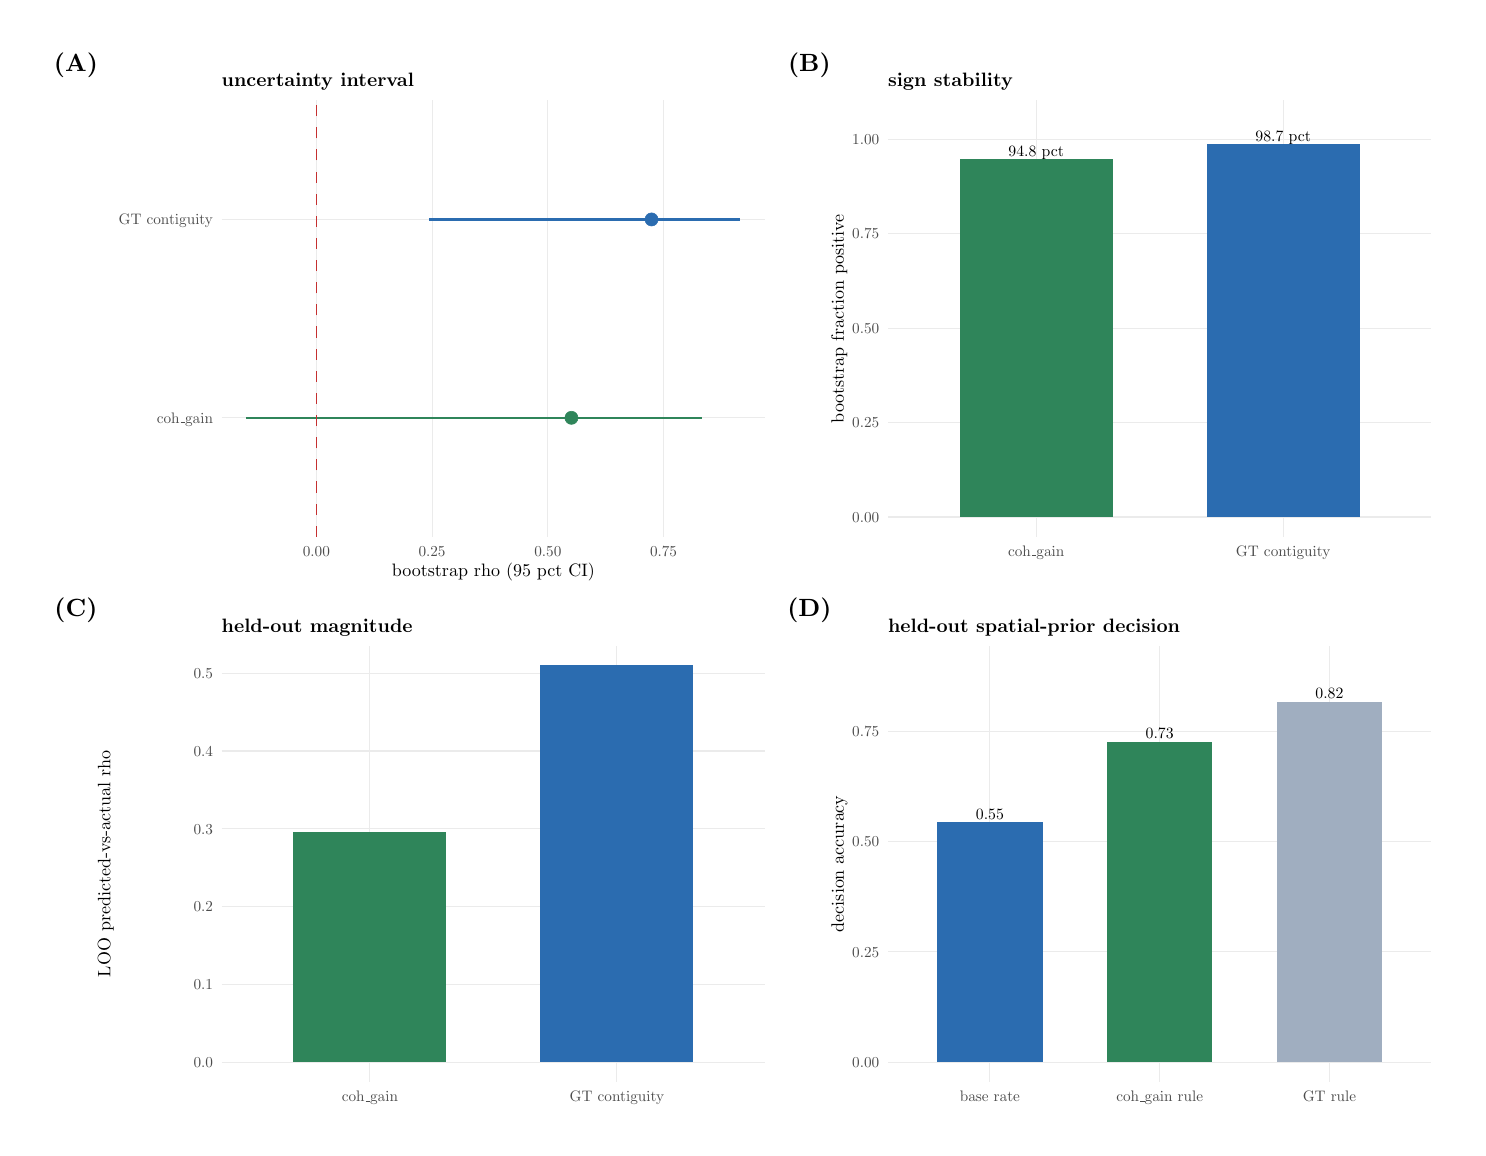
\begin{tikzpicture}[x=1pt,y=1pt]
\definecolor{fillColor}{RGB}{255,255,255}
\path[use as bounding box,fill=fillColor,fill opacity=0.00] (0,0) rectangle (516.73,397.48);
\begin{scope}
\path[clip] (  0.00,  0.00) rectangle (516.73,397.48);
\definecolor{drawColor}{RGB}{255,255,255}
\definecolor{fillColor}{RGB}{255,255,255}

\path[draw=drawColor,line width= 0.6pt,line join=round,line cap=round,fill=fillColor] (  0.00,  0.00) rectangle (516.73,397.48);
\end{scope}
\begin{scope}
\path[clip] (  5.50,195.00) rectangle (270.47,391.98);
\definecolor{fillColor}{RGB}{255,255,255}

\path[fill=fillColor] (  5.50,195.00) rectangle (270.47,391.99);
\end{scope}
\begin{scope}
\path[clip] (270.47,195.00) rectangle (511.23,391.98);
\definecolor{fillColor}{RGB}{255,255,255}

\path[fill=fillColor] (270.47,195.00) rectangle (511.23,391.99);
\end{scope}
\begin{scope}
\path[clip] (  5.50,  5.50) rectangle (270.47,195.00);
\definecolor{fillColor}{RGB}{255,255,255}

\path[fill=fillColor] (  5.50,  5.50) rectangle (270.47,195.00);
\end{scope}
\begin{scope}
\path[clip] (270.47,  5.50) rectangle (511.23,195.00);
\definecolor{fillColor}{RGB}{255,255,255}

\path[fill=fillColor] (270.47,  5.50) rectangle (511.23,195.00);
\end{scope}
\begin{scope}
\path[clip] ( 70.12,213.50) rectangle (266.47,371.19);
\definecolor{drawColor}{gray}{0.92}

\path[draw=drawColor,line width= 0.4pt,line join=round] ( 70.12,256.50) --
	(266.47,256.50);

\path[draw=drawColor,line width= 0.4pt,line join=round] ( 70.12,328.18) --
	(266.47,328.18);

\path[draw=drawColor,line width= 0.4pt,line join=round] (104.31,213.50) --
	(104.31,371.19);

\path[draw=drawColor,line width= 0.4pt,line join=round] (146.13,213.50) --
	(146.13,371.19);

\path[draw=drawColor,line width= 0.4pt,line join=round] (187.96,213.50) --
	(187.96,371.19);

\path[draw=drawColor,line width= 0.4pt,line join=round] (229.78,213.50) --
	(229.78,371.19);
\definecolor{drawColor}{RGB}{43,108,176}

\path[draw=drawColor,line width= 0.8pt,line join=round] (144.96,328.18) -- (257.55,328.18);
\definecolor{drawColor}{RGB}{47,133,90}

\path[draw=drawColor,line width= 0.8pt,line join=round] ( 79.05,256.50) -- (243.66,256.50);
\definecolor{drawColor}{RGB}{43,108,176}
\definecolor{fillColor}{RGB}{43,108,176}

\path[draw=drawColor,line width= 0.2pt,line join=round,line cap=round,fill=fillColor] (225.43,328.18) circle (  2.37);
\definecolor{drawColor}{RGB}{47,133,90}
\definecolor{fillColor}{RGB}{47,133,90}

\path[draw=drawColor,line width= 0.2pt,line join=round,line cap=round,fill=fillColor] (196.49,256.50) circle (  2.37);
\definecolor{drawColor}{RGB}{197,48,48}

\path[draw=drawColor,line width= 0.4pt,dash pattern=on 4pt off 4pt ,line join=round] (104.31,213.50) -- (104.31,371.19);
\end{scope}
\begin{scope}
\path[clip] (  0.00,  0.00) rectangle (516.73,397.48);
\definecolor{drawColor}{gray}{0.30}

\node[text=drawColor,anchor=base east,inner sep=0pt, outer sep=0pt, scale=  0.55] at ( 66.97,254.61) {coh{\_{}}gain};

\node[text=drawColor,anchor=base east,inner sep=0pt, outer sep=0pt, scale=  0.55] at ( 66.97,326.29) {GT contiguity};
\end{scope}
\begin{scope}
\path[clip] (  0.00,  0.00) rectangle (516.73,397.48);
\definecolor{drawColor}{gray}{0.30}

\node[text=drawColor,anchor=base,inner sep=0pt, outer sep=0pt, scale=  0.55] at (104.31,206.56) {0.00};

\node[text=drawColor,anchor=base,inner sep=0pt, outer sep=0pt, scale=  0.55] at (146.13,206.56) {0.25};

\node[text=drawColor,anchor=base,inner sep=0pt, outer sep=0pt, scale=  0.55] at (187.96,206.56) {0.50};

\node[text=drawColor,anchor=base,inner sep=0pt, outer sep=0pt, scale=  0.55] at (229.78,206.56) {0.75};
\end{scope}
\begin{scope}
\path[clip] (  0.00,  0.00) rectangle (516.73,397.48);
\definecolor{drawColor}{RGB}{0,0,0}

\node[text=drawColor,anchor=base,inner sep=0pt, outer sep=0pt, scale=  0.65] at (168.30,199.26) {bootstrap rho (95 pct CI)};
\end{scope}
\begin{scope}
\path[clip] (  0.00,  0.00) rectangle (516.73,397.48);
\definecolor{drawColor}{RGB}{0,0,0}

\node[text=drawColor,anchor=base west,inner sep=0pt, outer sep=0pt, scale=  0.70] at ( 70.12,376.05) {\bfseries uncertainty interval};
\end{scope}
\begin{scope}
\path[clip] (  0.00,  0.00) rectangle (516.73,397.48);
\definecolor{drawColor}{RGB}{0,0,0}

\node[text=drawColor,anchor=base,inner sep=0pt, outer sep=0pt, scale=  0.90] at ( 17.44,381.82) {\bfseries (A)};
\end{scope}
\begin{scope}
\path[clip] (310.88,213.50) rectangle (507.23,371.19);
\definecolor{drawColor}{gray}{0.92}

\path[draw=drawColor,line width= 0.4pt,line join=round] (310.88,220.66) --
	(507.23,220.66);

\path[draw=drawColor,line width= 0.4pt,line join=round] (310.88,254.80) --
	(507.23,254.80);

\path[draw=drawColor,line width= 0.4pt,line join=round] (310.88,288.93) --
	(507.23,288.93);

\path[draw=drawColor,line width= 0.4pt,line join=round] (310.88,323.06) --
	(507.23,323.06);

\path[draw=drawColor,line width= 0.4pt,line join=round] (310.88,357.19) --
	(507.23,357.19);

\path[draw=drawColor,line width= 0.4pt,line join=round] (364.43,213.50) --
	(364.43,371.19);

\path[draw=drawColor,line width= 0.4pt,line join=round] (453.68,213.50) --
	(453.68,371.19);
\definecolor{fillColor}{RGB}{43,108,176}

\path[fill=fillColor] (426.01,220.66) rectangle (481.35,355.42);
\definecolor{fillColor}{RGB}{47,133,90}

\path[fill=fillColor] (336.76,220.66) rectangle (392.10,350.10);
\definecolor{drawColor}{RGB}{0,0,0}

\node[text=drawColor,anchor=base,inner sep=0pt, outer sep=0pt, scale=  0.57] at (453.68,356.40) {98.7 pct};

\node[text=drawColor,anchor=base,inner sep=0pt, outer sep=0pt, scale=  0.57] at (364.43,351.08) {94.8 pct};
\end{scope}
\begin{scope}
\path[clip] (  0.00,  0.00) rectangle (516.73,397.48);
\definecolor{drawColor}{gray}{0.30}

\node[text=drawColor,anchor=base east,inner sep=0pt, outer sep=0pt, scale=  0.55] at (307.73,218.77) {0.00};

\node[text=drawColor,anchor=base east,inner sep=0pt, outer sep=0pt, scale=  0.55] at (307.73,252.90) {0.25};

\node[text=drawColor,anchor=base east,inner sep=0pt, outer sep=0pt, scale=  0.55] at (307.73,287.04) {0.50};

\node[text=drawColor,anchor=base east,inner sep=0pt, outer sep=0pt, scale=  0.55] at (307.73,321.17) {0.75};

\node[text=drawColor,anchor=base east,inner sep=0pt, outer sep=0pt, scale=  0.55] at (307.73,355.30) {1.00};
\end{scope}
\begin{scope}
\path[clip] (  0.00,  0.00) rectangle (516.73,397.48);
\definecolor{drawColor}{gray}{0.30}

\node[text=drawColor,anchor=base,inner sep=0pt, outer sep=0pt, scale=  0.55] at (364.43,206.56) {coh{\_{}}gain};

\node[text=drawColor,anchor=base,inner sep=0pt, outer sep=0pt, scale=  0.55] at (453.68,206.56) {GT contiguity};
\end{scope}
\begin{scope}
\path[clip] (  0.00,  0.00) rectangle (516.73,397.48);
\definecolor{drawColor}{RGB}{0,0,0}

\node[text=drawColor,rotate= 90.00,anchor=base,inner sep=0pt, outer sep=0pt, scale=  0.65] at (294.94,292.34) {bootstrap fraction positive};
\end{scope}
\begin{scope}
\path[clip] (  0.00,  0.00) rectangle (516.73,397.48);
\definecolor{drawColor}{RGB}{0,0,0}

\node[text=drawColor,anchor=base west,inner sep=0pt, outer sep=0pt, scale=  0.70] at (310.88,376.05) {\bfseries sign stability};
\end{scope}
\begin{scope}
\path[clip] (  0.00,  0.00) rectangle (516.73,397.48);
\definecolor{drawColor}{RGB}{0,0,0}

\node[text=drawColor,anchor=base,inner sep=0pt, outer sep=0pt, scale=  0.90] at (282.47,381.82) {\bfseries (B)};
\end{scope}
\begin{scope}
\path[clip] ( 70.12, 16.51) rectangle (266.47,174.20);
\definecolor{drawColor}{gray}{0.92}

\path[draw=drawColor,line width= 0.4pt,line join=round] ( 70.12, 23.68) --
	(266.47, 23.68);

\path[draw=drawColor,line width= 0.4pt,line join=round] ( 70.12, 51.79) --
	(266.47, 51.79);

\path[draw=drawColor,line width= 0.4pt,line join=round] ( 70.12, 79.89) --
	(266.47, 79.89);

\path[draw=drawColor,line width= 0.4pt,line join=round] ( 70.12,108.00) --
	(266.47,108.00);

\path[draw=drawColor,line width= 0.4pt,line join=round] ( 70.12,136.11) --
	(266.47,136.11);

\path[draw=drawColor,line width= 0.4pt,line join=round] ( 70.12,164.22) --
	(266.47,164.22);

\path[draw=drawColor,line width= 0.4pt,line join=round] (123.67, 16.51) --
	(123.67,174.20);

\path[draw=drawColor,line width= 0.4pt,line join=round] (212.92, 16.51) --
	(212.92,174.20);
\definecolor{fillColor}{RGB}{43,108,176}

\path[fill=fillColor] (185.26, 23.68) rectangle (240.59,167.03);
\definecolor{fillColor}{RGB}{47,133,90}

\path[fill=fillColor] ( 96.01, 23.68) rectangle (151.34,106.88);
\end{scope}
\begin{scope}
\path[clip] (  0.00,  0.00) rectangle (516.73,397.48);
\definecolor{drawColor}{gray}{0.30}

\node[text=drawColor,anchor=base east,inner sep=0pt, outer sep=0pt, scale=  0.55] at ( 66.97, 21.78) {0.0};

\node[text=drawColor,anchor=base east,inner sep=0pt, outer sep=0pt, scale=  0.55] at ( 66.97, 49.89) {0.1};

\node[text=drawColor,anchor=base east,inner sep=0pt, outer sep=0pt, scale=  0.55] at ( 66.97, 78.00) {0.2};

\node[text=drawColor,anchor=base east,inner sep=0pt, outer sep=0pt, scale=  0.55] at ( 66.97,106.11) {0.3};

\node[text=drawColor,anchor=base east,inner sep=0pt, outer sep=0pt, scale=  0.55] at ( 66.97,134.22) {0.4};

\node[text=drawColor,anchor=base east,inner sep=0pt, outer sep=0pt, scale=  0.55] at ( 66.97,162.33) {0.5};
\end{scope}
\begin{scope}
\path[clip] (  0.00,  0.00) rectangle (516.73,397.48);
\definecolor{drawColor}{gray}{0.30}

\node[text=drawColor,anchor=base,inner sep=0pt, outer sep=0pt, scale=  0.55] at (123.67,  9.57) {coh{\_{}}gain};

\node[text=drawColor,anchor=base,inner sep=0pt, outer sep=0pt, scale=  0.55] at (212.92,  9.57) {GT contiguity};
\end{scope}
\begin{scope}
\path[clip] (  0.00,  0.00) rectangle (516.73,397.48);
\definecolor{drawColor}{RGB}{0,0,0}

\node[text=drawColor,rotate= 90.00,anchor=base,inner sep=0pt, outer sep=0pt, scale=  0.65] at ( 29.85, 95.35) {LOO predicted-vs-actual rho};
\end{scope}
\begin{scope}
\path[clip] (  0.00,  0.00) rectangle (516.73,397.48);
\definecolor{drawColor}{RGB}{0,0,0}

\node[text=drawColor,anchor=base west,inner sep=0pt, outer sep=0pt, scale=  0.70] at ( 70.12,179.06) {\bfseries held-out magnitude};
\end{scope}
\begin{scope}
\path[clip] (  0.00,  0.00) rectangle (516.73,397.48);
\definecolor{drawColor}{RGB}{0,0,0}

\node[text=drawColor,anchor=base,inner sep=0pt, outer sep=0pt, scale=  0.90] at ( 17.44,184.83) {\bfseries (C)};
\end{scope}
\begin{scope}
\path[clip] (310.88, 16.51) rectangle (507.23,174.20);
\definecolor{drawColor}{gray}{0.92}

\path[draw=drawColor,line width= 0.4pt,line join=round] (310.88, 23.68) --
	(507.23, 23.68);

\path[draw=drawColor,line width= 0.4pt,line join=round] (310.88, 63.50) --
	(507.23, 63.50);

\path[draw=drawColor,line width= 0.4pt,line join=round] (310.88,103.32) --
	(507.23,103.32);

\path[draw=drawColor,line width= 0.4pt,line join=round] (310.88,143.14) --
	(507.23,143.14);

\path[draw=drawColor,line width= 0.4pt,line join=round] (347.70, 16.51) --
	(347.70,174.20);

\path[draw=drawColor,line width= 0.4pt,line join=round] (409.06, 16.51) --
	(409.06,174.20);

\path[draw=drawColor,line width= 0.4pt,line join=round] (470.41, 16.51) --
	(470.41,174.20);
\definecolor{fillColor}{RGB}{160,174,192}

\path[fill=fillColor] (451.39, 23.68) rectangle (489.44,153.97);
\definecolor{fillColor}{RGB}{47,133,90}

\path[fill=fillColor] (390.03, 23.68) rectangle (428.08,139.48);
\definecolor{fillColor}{RGB}{43,108,176}

\path[fill=fillColor] (328.67, 23.68) rectangle (366.72,110.49);
\definecolor{drawColor}{RGB}{0,0,0}

\node[text=drawColor,anchor=base,inner sep=0pt, outer sep=0pt, scale=  0.57] at (470.41,154.95) {0.82};

\node[text=drawColor,anchor=base,inner sep=0pt, outer sep=0pt, scale=  0.57] at (409.06,140.46) {0.73};

\node[text=drawColor,anchor=base,inner sep=0pt, outer sep=0pt, scale=  0.57] at (347.70,111.47) {0.55};
\end{scope}
\begin{scope}
\path[clip] (  0.00,  0.00) rectangle (516.73,397.48);
\definecolor{drawColor}{gray}{0.30}

\node[text=drawColor,anchor=base east,inner sep=0pt, outer sep=0pt, scale=  0.55] at (307.73, 21.78) {0.00};

\node[text=drawColor,anchor=base east,inner sep=0pt, outer sep=0pt, scale=  0.55] at (307.73, 61.60) {0.25};

\node[text=drawColor,anchor=base east,inner sep=0pt, outer sep=0pt, scale=  0.55] at (307.73,101.42) {0.50};

\node[text=drawColor,anchor=base east,inner sep=0pt, outer sep=0pt, scale=  0.55] at (307.73,141.25) {0.75};
\end{scope}
\begin{scope}
\path[clip] (  0.00,  0.00) rectangle (516.73,397.48);
\definecolor{drawColor}{gray}{0.30}

\node[text=drawColor,anchor=base,inner sep=0pt, outer sep=0pt, scale=  0.55] at (347.70,  9.57) {base rate};

\node[text=drawColor,anchor=base,inner sep=0pt, outer sep=0pt, scale=  0.55] at (409.06,  9.57) {coh{\_{}}gain rule};

\node[text=drawColor,anchor=base,inner sep=0pt, outer sep=0pt, scale=  0.55] at (470.41,  9.57) {GT rule};
\end{scope}
\begin{scope}
\path[clip] (  0.00,  0.00) rectangle (516.73,397.48);
\definecolor{drawColor}{RGB}{0,0,0}

\node[text=drawColor,rotate= 90.00,anchor=base,inner sep=0pt, outer sep=0pt, scale=  0.65] at (294.94, 95.35) {decision accuracy};
\end{scope}
\begin{scope}
\path[clip] (  0.00,  0.00) rectangle (516.73,397.48);
\definecolor{drawColor}{RGB}{0,0,0}

\node[text=drawColor,anchor=base west,inner sep=0pt, outer sep=0pt, scale=  0.70] at (310.88,179.06) {\bfseries held-out spatial-prior decision};
\end{scope}
\begin{scope}
\path[clip] (  0.00,  0.00) rectangle (516.73,397.48);
\definecolor{drawColor}{RGB}{0,0,0}

\node[text=drawColor,anchor=base,inner sep=0pt, outer sep=0pt, scale=  0.90] at (282.47,184.83) {\bfseries (D)};
\end{scope}
\end{tikzpicture}
}
\caption{Robustness of the law: (a) 10k-dataset bootstrap 95\% CIs for the GT-based and label-free
correlations; (b) leave-one-dataset-out is predictive and the decision rule beats its base rate, even
label-free.}
\label{fig:robust}
\end{figure}

\section{The law is causal and deployable without labels}\label{sec:causal}
\paragraph{Causal.} We manipulate \emph{only} contiguity on synthetic tissue: scrambling a fraction of cells'
positions while each keeps its expression and label holds the expression-to-label map fixed, so the
non-spatial floor's ARI stays at 0.345 throughout. Spatial-prior advantage then rises with contiguity and
flips sign (Fig.~\ref{fig:mech}): $\rho=+0.98$ for the neighbour-mean smoother and $+1.00$ for STAGATE.
Since contiguity is the only variable we change, this is causal evidence that contiguity drives the value
of a spatial prior; the learned-GNN arm bears most of this conclusion, while the neighbour-mean arm mainly
illustrates the mechanism, though STAGATE's graph-attention mechanism is itself an adaptive form of
neighbour-averaging over the same spatial $k$NN graph used to define contiguity, so the two arms should be
read as correlated rather than architecturally independent confirmations; the causal identification of
contiguity's effect (via exogenous scrambling) holds regardless.

\paragraph{Label-free.} The law as stated still needs the ground truth it is meant to replace. The obvious
label-free proxies, Moran's $I$ of expression and the unsupervised kNN same-cluster fraction, invert
($\rho=-0.34$ and $-0.42$ versus advantage): raw-expression smoothness reflects cell-type structure, not
domain contiguity (Fig.~\ref{fig:proxy}). Our proxy \texttt{coh\_gain}, the extra spatial coherence
unsupervised clustering gains under smoothing, recovers the correct sign ($\rho=+0.55$ versus advantage,
$+0.56$ versus contiguity) and beats the base rate out-of-sample. It recovers the direction of the law, but
not the oracle's significance: once we account for having selected it as the best of six candidate proxies
(a Westfall--Young max-statistic permutation test, $B{=}10{,}000$), the effect is not significant
(search-corrected $p=0.28$; uncorrected per-candidate $p=0.079$). \texttt{coh\_gain} should therefore be read
as a directional, honestly marginal label-free prior, with the causal synthetic sweep above
(\S\ref{sec:causal}, $\rho=+0.98$ to $+1.00$, $p<0.001$) carrying the primary weight.

\begin{figure}[htbp]\centering
\resizebox{0.82\linewidth}{!}{% !TEX encoding = UTF-8 Unicode
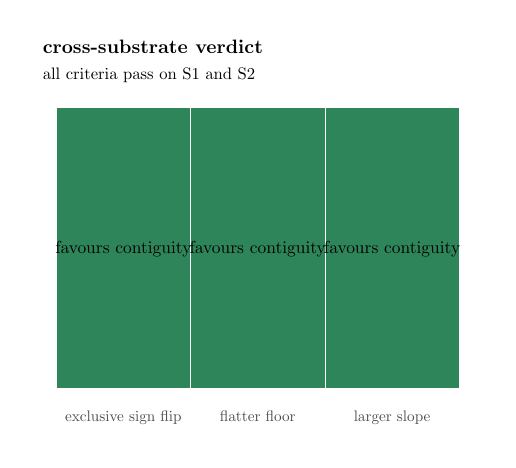
\begin{tikzpicture}[x=1pt,y=1pt]
\definecolor{fillColor}{RGB}{255,255,255}
\path[use as bounding box,fill=fillColor,fill opacity=0.00] (0,0) rectangle (166.27,148.95);
\begin{scope}
\path[clip] (  1.45,  1.65) rectangle (164.83,147.30);
\definecolor{fillColor}{RGB}{255,255,255}

\path[fill=fillColor] (  1.45,  1.65) rectangle (164.83,147.30);
\end{scope}
\begin{scope}
\path[clip] (  5.45, 13.45) rectangle (160.83,125.47);
\definecolor{drawColor}{RGB}{255,255,255}
\definecolor{fillColor}{RGB}{47,133,90}

\path[draw=drawColor,line width= 0.1pt,fill=fillColor] (107.41, 18.54) rectangle (155.97,120.37);

\path[draw=drawColor,line width= 0.1pt,fill=fillColor] ( 10.30, 18.54) rectangle ( 58.86,120.37);

\path[draw=drawColor,line width= 0.1pt,fill=fillColor] ( 58.86, 18.54) rectangle (107.41,120.37);
\definecolor{drawColor}{RGB}{0,0,0}

\node[text=drawColor,anchor=base,inner sep=0pt, outer sep=0pt, scale=  0.63] at (131.69, 67.30) {favours contiguity};

\node[text=drawColor,anchor=base,inner sep=0pt, outer sep=0pt, scale=  0.63] at ( 34.58, 67.30) {favours contiguity};

\node[text=drawColor,anchor=base,inner sep=0pt, outer sep=0pt, scale=  0.63] at ( 83.14, 67.30) {favours contiguity};
\end{scope}
\begin{scope}
\path[clip] (  0.00,  0.00) rectangle (166.27,148.95);
\definecolor{drawColor}{gray}{0.30}

\node[text=drawColor,anchor=base,inner sep=0pt, outer sep=0pt, scale=  0.55] at ( 34.58,  6.51) {exclusive sign flip};

\node[text=drawColor,anchor=base,inner sep=0pt, outer sep=0pt, scale=  0.55] at ( 83.14,  6.51) {flatter floor};

\node[text=drawColor,anchor=base,inner sep=0pt, outer sep=0pt, scale=  0.55] at (131.69,  6.51) {larger slope};
\end{scope}
\begin{scope}
\path[clip] (  0.00,  0.00) rectangle (166.27,148.95);
\definecolor{drawColor}{RGB}{0,0,0}

\node[text=drawColor,anchor=base west,inner sep=0pt, outer sep=0pt, scale=  0.60] at (  5.45,130.29) {all criteria pass on S1 and S2};
\end{scope}
\begin{scope}
\path[clip] (  0.00,  0.00) rectangle (166.27,148.95);
\definecolor{drawColor}{RGB}{0,0,0}

\node[text=drawColor,anchor=base west,inner sep=0pt, outer sep=0pt, scale=  0.70] at (  5.45,139.47) {\bfseries cross-substrate verdict};
\end{scope}
\end{tikzpicture}
}
\caption{Controlled mechanism: with the expression signal held fixed (flat grey control), spatial-prior
advantage rises with manipulated contiguity and flips sign, giving causal evidence for the law.}
\label{fig:mech}
\end{figure}

\begin{figure}[htbp]\centering
\resizebox{0.80\linewidth}{!}{% !TEX encoding = UTF-8 Unicode
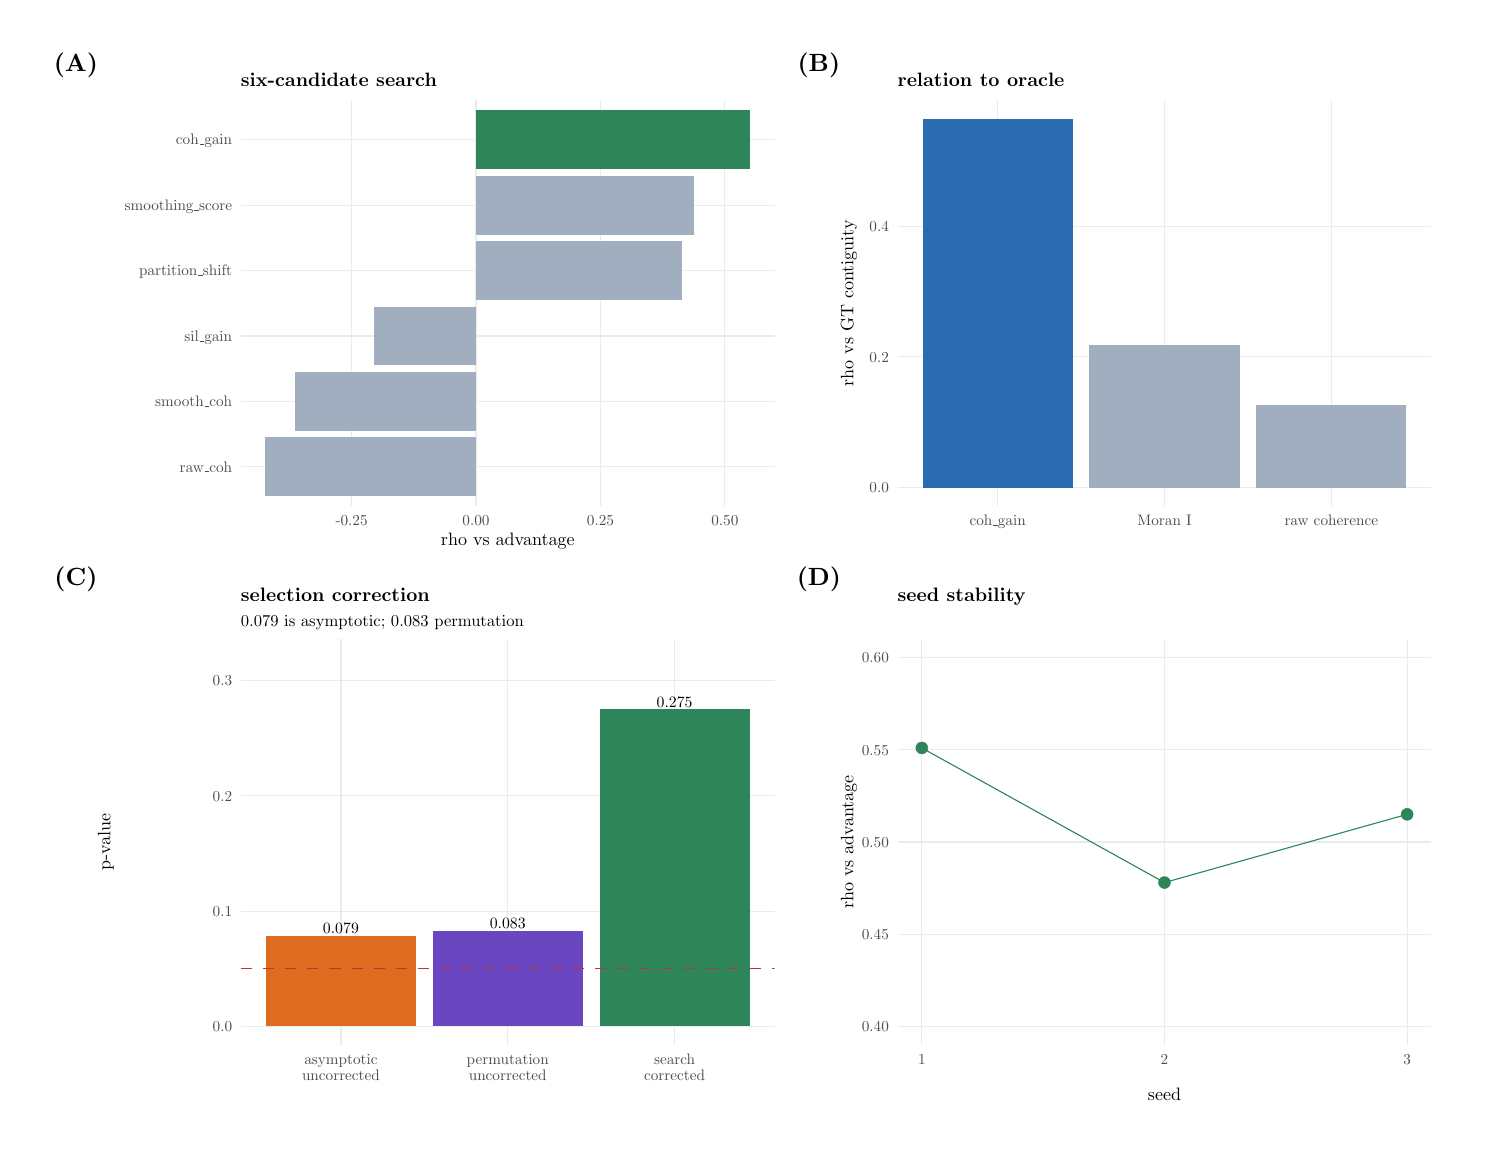
\begin{tikzpicture}[x=1pt,y=1pt]
\definecolor{fillColor}{RGB}{255,255,255}
\path[use as bounding box,fill=fillColor,fill opacity=0.00] (0,0) rectangle (516.73,397.48);
\begin{scope}
\path[clip] (  0.00,  0.00) rectangle (516.73,397.48);
\definecolor{drawColor}{RGB}{255,255,255}
\definecolor{fillColor}{RGB}{255,255,255}

\path[draw=drawColor,line width= 0.6pt,line join=round,line cap=round,fill=fillColor] (  0.00,  0.00) rectangle (516.73,397.48);
\end{scope}
\begin{scope}
\path[clip] (  5.50,206.11) rectangle (273.93,391.98);
\definecolor{fillColor}{RGB}{255,255,255}

\path[fill=fillColor] (  5.50,206.11) rectangle (273.93,391.98);
\end{scope}
\begin{scope}
\path[clip] (273.93,206.11) rectangle (511.23,391.98);
\definecolor{fillColor}{RGB}{255,255,255}

\path[fill=fillColor] (273.93,206.11) rectangle (511.23,391.98);
\end{scope}
\begin{scope}
\path[clip] (  5.50,  5.50) rectangle (273.93,206.11);
\definecolor{fillColor}{RGB}{255,255,255}

\path[fill=fillColor] (  5.50,  5.50) rectangle (273.93,206.11);
\end{scope}
\begin{scope}
\path[clip] (273.93,  5.50) rectangle (511.23,206.11);
\definecolor{fillColor}{RGB}{255,255,255}

\path[fill=fillColor] (273.93,  5.50) rectangle (511.23,206.11);
\end{scope}
\begin{scope}
\path[clip] ( 77.04,224.61) rectangle (269.93,371.19);
\definecolor{drawColor}{gray}{0.92}

\path[draw=drawColor,line width= 0.4pt,line join=round] ( 77.04,238.80) --
	(269.93,238.80);

\path[draw=drawColor,line width= 0.4pt,line join=round] ( 77.04,262.44) --
	(269.93,262.44);

\path[draw=drawColor,line width= 0.4pt,line join=round] ( 77.04,286.08) --
	(269.93,286.08);

\path[draw=drawColor,line width= 0.4pt,line join=round] ( 77.04,309.72) --
	(269.93,309.72);

\path[draw=drawColor,line width= 0.4pt,line join=round] ( 77.04,333.36) --
	(269.93,333.36);

\path[draw=drawColor,line width= 0.4pt,line join=round] ( 77.04,357.00) --
	(269.93,357.00);

\path[draw=drawColor,line width= 0.4pt,line join=round] (117.05,224.61) --
	(117.05,371.19);

\path[draw=drawColor,line width= 0.4pt,line join=round] (162.01,224.61) --
	(162.01,371.19);

\path[draw=drawColor,line width= 0.4pt,line join=round] (206.98,224.61) --
	(206.98,371.19);

\path[draw=drawColor,line width= 0.4pt,line join=round] (251.94,224.61) --
	(251.94,371.19);
\definecolor{fillColor}{RGB}{160,174,192}

\path[fill=fillColor] ( 85.80,228.16) rectangle (162.01,249.44);

\path[fill=fillColor] ( 96.46,251.80) rectangle (162.01,273.08);
\definecolor{fillColor}{RGB}{47,133,90}

\path[fill=fillColor] (162.01,346.37) rectangle (261.16,367.64);
\definecolor{fillColor}{RGB}{160,174,192}

\path[fill=fillColor] (162.01,299.08) rectangle (236.58,320.36);

\path[fill=fillColor] (125.14,275.44) rectangle (162.01,296.72);

\path[fill=fillColor] (162.01,322.72) rectangle (240.68,344.00);
\end{scope}
\begin{scope}
\path[clip] (  0.00,  0.00) rectangle (516.73,397.48);
\definecolor{drawColor}{gray}{0.30}

\node[text=drawColor,anchor=base east,inner sep=0pt, outer sep=0pt, scale=  0.55] at ( 73.89,236.90) {raw{\_{}}coh};

\node[text=drawColor,anchor=base east,inner sep=0pt, outer sep=0pt, scale=  0.55] at ( 73.89,260.54) {smooth{\_{}}coh};

\node[text=drawColor,anchor=base east,inner sep=0pt, outer sep=0pt, scale=  0.55] at ( 73.89,284.19) {sil{\_{}}gain};

\node[text=drawColor,anchor=base east,inner sep=0pt, outer sep=0pt, scale=  0.55] at ( 73.89,307.83) {partition{\_{}}shift};

\node[text=drawColor,anchor=base east,inner sep=0pt, outer sep=0pt, scale=  0.55] at ( 73.89,331.47) {smoothing{\_{}}score};

\node[text=drawColor,anchor=base east,inner sep=0pt, outer sep=0pt, scale=  0.55] at ( 73.89,355.11) {coh{\_{}}gain};
\end{scope}
\begin{scope}
\path[clip] (  0.00,  0.00) rectangle (516.73,397.48);
\definecolor{drawColor}{gray}{0.30}

\node[text=drawColor,anchor=base,inner sep=0pt, outer sep=0pt, scale=  0.55] at (117.05,217.67) {-0.25};

\node[text=drawColor,anchor=base,inner sep=0pt, outer sep=0pt, scale=  0.55] at (162.01,217.67) {0.00};

\node[text=drawColor,anchor=base,inner sep=0pt, outer sep=0pt, scale=  0.55] at (206.98,217.67) {0.25};

\node[text=drawColor,anchor=base,inner sep=0pt, outer sep=0pt, scale=  0.55] at (251.94,217.67) {0.50};
\end{scope}
\begin{scope}
\path[clip] (  0.00,  0.00) rectangle (516.73,397.48);
\definecolor{drawColor}{RGB}{0,0,0}

\node[text=drawColor,anchor=base,inner sep=0pt, outer sep=0pt, scale=  0.65] at (173.48,210.38) {rho vs advantage};
\end{scope}
\begin{scope}
\path[clip] (  0.00,  0.00) rectangle (516.73,397.48);
\definecolor{drawColor}{RGB}{0,0,0}

\node[text=drawColor,anchor=base west,inner sep=0pt, outer sep=0pt, scale=  0.70] at ( 77.04,376.05) {\bfseries six-candidate search};
\end{scope}
\begin{scope}
\path[clip] (  0.00,  0.00) rectangle (516.73,397.48);
\definecolor{drawColor}{RGB}{0,0,0}

\node[text=drawColor,anchor=base,inner sep=0pt, outer sep=0pt, scale=  0.90] at ( 17.44,381.82) {\bfseries (A)};
\end{scope}
\begin{scope}
\path[clip] (314.34,224.61) rectangle (507.23,371.19);
\definecolor{drawColor}{gray}{0.92}

\path[draw=drawColor,line width= 0.4pt,line join=round] (314.34,231.27) --
	(507.23,231.27);

\path[draw=drawColor,line width= 0.4pt,line join=round] (314.34,278.53) --
	(507.23,278.53);

\path[draw=drawColor,line width= 0.4pt,line join=round] (314.34,325.78) --
	(507.23,325.78);

\path[draw=drawColor,line width= 0.4pt,line join=round] (350.50,224.61) --
	(350.50,371.19);

\path[draw=drawColor,line width= 0.4pt,line join=round] (410.78,224.61) --
	(410.78,371.19);

\path[draw=drawColor,line width= 0.4pt,line join=round] (471.06,224.61) --
	(471.06,371.19);
\definecolor{fillColor}{RGB}{160,174,192}

\path[fill=fillColor] (383.66,231.27) rectangle (437.91,282.78);

\path[fill=fillColor] (443.94,231.27) rectangle (498.19,261.28);
\definecolor{fillColor}{RGB}{43,108,176}

\path[fill=fillColor] (323.38,231.27) rectangle (377.63,364.53);
\end{scope}
\begin{scope}
\path[clip] (  0.00,  0.00) rectangle (516.73,397.48);
\definecolor{drawColor}{gray}{0.30}

\node[text=drawColor,anchor=base east,inner sep=0pt, outer sep=0pt, scale=  0.55] at (311.19,229.38) {0.0};

\node[text=drawColor,anchor=base east,inner sep=0pt, outer sep=0pt, scale=  0.55] at (311.19,276.63) {0.2};

\node[text=drawColor,anchor=base east,inner sep=0pt, outer sep=0pt, scale=  0.55] at (311.19,323.89) {0.4};
\end{scope}
\begin{scope}
\path[clip] (  0.00,  0.00) rectangle (516.73,397.48);
\definecolor{drawColor}{gray}{0.30}

\node[text=drawColor,anchor=base,inner sep=0pt, outer sep=0pt, scale=  0.55] at (350.50,217.67) {coh{\_{}}gain};

\node[text=drawColor,anchor=base,inner sep=0pt, outer sep=0pt, scale=  0.55] at (410.78,217.67) {Moran I};

\node[text=drawColor,anchor=base,inner sep=0pt, outer sep=0pt, scale=  0.55] at (471.06,217.67) {raw coherence};
\end{scope}
\begin{scope}
\path[clip] (  0.00,  0.00) rectangle (516.73,397.48);
\definecolor{drawColor}{RGB}{0,0,0}

\node[text=drawColor,rotate= 90.00,anchor=base,inner sep=0pt, outer sep=0pt, scale=  0.65] at (298.39,297.90) {rho vs GT contiguity};
\end{scope}
\begin{scope}
\path[clip] (  0.00,  0.00) rectangle (516.73,397.48);
\definecolor{drawColor}{RGB}{0,0,0}

\node[text=drawColor,anchor=base west,inner sep=0pt, outer sep=0pt, scale=  0.70] at (314.34,376.05) {\bfseries relation to oracle};
\end{scope}
\begin{scope}
\path[clip] (  0.00,  0.00) rectangle (516.73,397.48);
\definecolor{drawColor}{RGB}{0,0,0}

\node[text=drawColor,anchor=base,inner sep=0pt, outer sep=0pt, scale=  0.90] at (285.92,381.82) {\bfseries (B)};
\end{scope}
\begin{scope}
\path[clip] ( 77.04, 29.94) rectangle (269.93,176.52);
\definecolor{drawColor}{gray}{0.92}

\path[draw=drawColor,line width= 0.4pt,line join=round] ( 77.04, 36.60) --
	(269.93, 36.60);

\path[draw=drawColor,line width= 0.4pt,line join=round] ( 77.04, 78.24) --
	(269.93, 78.24);

\path[draw=drawColor,line width= 0.4pt,line join=round] ( 77.04,119.88) --
	(269.93,119.88);

\path[draw=drawColor,line width= 0.4pt,line join=round] ( 77.04,161.53) --
	(269.93,161.53);

\path[draw=drawColor,line width= 0.4pt,line join=round] (113.20, 29.94) --
	(113.20,176.52);

\path[draw=drawColor,line width= 0.4pt,line join=round] (173.48, 29.94) --
	(173.48,176.52);

\path[draw=drawColor,line width= 0.4pt,line join=round] (233.76, 29.94) --
	(233.76,176.52);
\definecolor{fillColor}{RGB}{221,107,32}

\path[fill=fillColor] ( 86.08, 36.60) rectangle (140.33, 69.42);
\definecolor{fillColor}{RGB}{107,70,193}

\path[fill=fillColor] (146.36, 36.60) rectangle (200.61, 71.16);
\definecolor{fillColor}{RGB}{47,133,90}

\path[fill=fillColor] (206.64, 36.60) rectangle (260.89,151.12);
\definecolor{drawColor}{RGB}{197,48,48}

\path[draw=drawColor,line width= 0.4pt,dash pattern=on 4pt off 4pt ,line join=round] ( 77.04, 57.42) -- (269.93, 57.42);
\definecolor{drawColor}{RGB}{0,0,0}

\node[text=drawColor,anchor=base,inner sep=0pt, outer sep=0pt, scale=  0.57] at (113.20, 70.20) {0.079};

\node[text=drawColor,anchor=base,inner sep=0pt, outer sep=0pt, scale=  0.57] at (173.48, 71.95) {0.083};

\node[text=drawColor,anchor=base,inner sep=0pt, outer sep=0pt, scale=  0.57] at (233.76,151.90) {0.275};
\end{scope}
\begin{scope}
\path[clip] (  0.00,  0.00) rectangle (516.73,397.48);
\definecolor{drawColor}{gray}{0.30}

\node[text=drawColor,anchor=base east,inner sep=0pt, outer sep=0pt, scale=  0.55] at ( 73.89, 34.71) {0.0};

\node[text=drawColor,anchor=base east,inner sep=0pt, outer sep=0pt, scale=  0.55] at ( 73.89, 76.35) {0.1};

\node[text=drawColor,anchor=base east,inner sep=0pt, outer sep=0pt, scale=  0.55] at ( 73.89,117.99) {0.2};

\node[text=drawColor,anchor=base east,inner sep=0pt, outer sep=0pt, scale=  0.55] at ( 73.89,159.63) {0.3};
\end{scope}
\begin{scope}
\path[clip] (  0.00,  0.00) rectangle (516.73,397.48);
\definecolor{drawColor}{gray}{0.30}

\node[text=drawColor,anchor=base,inner sep=0pt, outer sep=0pt, scale=  0.55] at (113.20, 23.00) {asymptotic};

\node[text=drawColor,anchor=base,inner sep=0pt, outer sep=0pt, scale=  0.55] at (113.20, 17.06) {uncorrected};

\node[text=drawColor,anchor=base,inner sep=0pt, outer sep=0pt, scale=  0.55] at (173.48, 23.00) {permutation};

\node[text=drawColor,anchor=base,inner sep=0pt, outer sep=0pt, scale=  0.55] at (173.48, 17.06) {uncorrected};

\node[text=drawColor,anchor=base,inner sep=0pt, outer sep=0pt, scale=  0.55] at (233.76, 23.00) {search};

\node[text=drawColor,anchor=base,inner sep=0pt, outer sep=0pt, scale=  0.55] at (233.76, 17.06) {corrected};
\end{scope}
\begin{scope}
\path[clip] (  0.00,  0.00) rectangle (516.73,397.48);
\definecolor{drawColor}{RGB}{0,0,0}

\node[text=drawColor,rotate= 90.00,anchor=base,inner sep=0pt, outer sep=0pt, scale=  0.65] at ( 29.85,103.23) {p-value};
\end{scope}
\begin{scope}
\path[clip] (  0.00,  0.00) rectangle (516.73,397.48);
\definecolor{drawColor}{RGB}{0,0,0}

\node[text=drawColor,anchor=base west,inner sep=0pt, outer sep=0pt, scale=  0.60] at ( 77.04,181.18) {0.079 is asymptotic; 0.083 permutation};
\end{scope}
\begin{scope}
\path[clip] (  0.00,  0.00) rectangle (516.73,397.48);
\definecolor{drawColor}{RGB}{0,0,0}

\node[text=drawColor,anchor=base west,inner sep=0pt, outer sep=0pt, scale=  0.70] at ( 77.04,190.18) {\bfseries selection correction};
\end{scope}
\begin{scope}
\path[clip] (  0.00,  0.00) rectangle (516.73,397.48);
\definecolor{drawColor}{RGB}{0,0,0}

\node[text=drawColor,anchor=base,inner sep=0pt, outer sep=0pt, scale=  0.90] at ( 17.44,195.95) {\bfseries (C)};
\end{scope}
\begin{scope}
\path[clip] (314.34, 29.94) rectangle (507.23,176.52);
\definecolor{drawColor}{gray}{0.92}

\path[draw=drawColor,line width= 0.4pt,line join=round] (314.34, 36.60) --
	(507.23, 36.60);

\path[draw=drawColor,line width= 0.4pt,line join=round] (314.34, 69.92) --
	(507.23, 69.92);

\path[draw=drawColor,line width= 0.4pt,line join=round] (314.34,103.23) --
	(507.23,103.23);

\path[draw=drawColor,line width= 0.4pt,line join=round] (314.34,136.54) --
	(507.23,136.54);

\path[draw=drawColor,line width= 0.4pt,line join=round] (314.34,169.85) --
	(507.23,169.85);

\path[draw=drawColor,line width= 0.4pt,line join=round] (323.10, 29.94) --
	(323.10,176.52);

\path[draw=drawColor,line width= 0.4pt,line join=round] (410.78, 29.94) --
	(410.78,176.52);

\path[draw=drawColor,line width= 0.4pt,line join=round] (498.46, 29.94) --
	(498.46,176.52);
\definecolor{drawColor}{RGB}{47,133,90}

\path[draw=drawColor,line width= 0.4pt,line join=round] (323.10,137.21) --
	(410.78, 88.57) --
	(498.46,113.22);
\definecolor{fillColor}{RGB}{47,133,90}

\path[draw=drawColor,line width= 0.2pt,line join=round,line cap=round,fill=fillColor] (323.10,137.21) circle (  2.15);

\path[draw=drawColor,line width= 0.2pt,line join=round,line cap=round,fill=fillColor] (410.78, 88.57) circle (  2.15);

\path[draw=drawColor,line width= 0.2pt,line join=round,line cap=round,fill=fillColor] (498.46,113.22) circle (  2.15);
\end{scope}
\begin{scope}
\path[clip] (  0.00,  0.00) rectangle (516.73,397.48);
\definecolor{drawColor}{gray}{0.30}

\node[text=drawColor,anchor=base east,inner sep=0pt, outer sep=0pt, scale=  0.55] at (311.19, 34.71) {0.40};

\node[text=drawColor,anchor=base east,inner sep=0pt, outer sep=0pt, scale=  0.55] at (311.19, 68.02) {0.45};

\node[text=drawColor,anchor=base east,inner sep=0pt, outer sep=0pt, scale=  0.55] at (311.19,101.33) {0.50};

\node[text=drawColor,anchor=base east,inner sep=0pt, outer sep=0pt, scale=  0.55] at (311.19,134.65) {0.55};

\node[text=drawColor,anchor=base east,inner sep=0pt, outer sep=0pt, scale=  0.55] at (311.19,167.96) {0.60};
\end{scope}
\begin{scope}
\path[clip] (  0.00,  0.00) rectangle (516.73,397.48);
\definecolor{drawColor}{gray}{0.30}

\node[text=drawColor,anchor=base,inner sep=0pt, outer sep=0pt, scale=  0.55] at (323.10, 23.00) {1};

\node[text=drawColor,anchor=base,inner sep=0pt, outer sep=0pt, scale=  0.55] at (410.78, 23.00) {2};

\node[text=drawColor,anchor=base,inner sep=0pt, outer sep=0pt, scale=  0.55] at (498.46, 23.00) {3};
\end{scope}
\begin{scope}
\path[clip] (  0.00,  0.00) rectangle (516.73,397.48);
\definecolor{drawColor}{RGB}{0,0,0}

\node[text=drawColor,anchor=base,inner sep=0pt, outer sep=0pt, scale=  0.65] at (410.78,  9.76) {seed};
\end{scope}
\begin{scope}
\path[clip] (  0.00,  0.00) rectangle (516.73,397.48);
\definecolor{drawColor}{RGB}{0,0,0}

\node[text=drawColor,rotate= 90.00,anchor=base,inner sep=0pt, outer sep=0pt, scale=  0.65] at (298.39,103.23) {rho vs advantage};
\end{scope}
\begin{scope}
\path[clip] (  0.00,  0.00) rectangle (516.73,397.48);
\definecolor{drawColor}{RGB}{0,0,0}

\node[text=drawColor,anchor=base west,inner sep=0pt, outer sep=0pt, scale=  0.70] at (314.34,190.18) {\bfseries seed stability};
\end{scope}
\begin{scope}
\path[clip] (  0.00,  0.00) rectangle (516.73,397.48);
\definecolor{drawColor}{RGB}{0,0,0}

\node[text=drawColor,anchor=base,inner sep=0pt, outer sep=0pt, scale=  0.90] at (285.92,195.95) {\bfseries (D)};
\end{scope}
\end{tikzpicture}
}
\caption{Label-free proxy search: naive expression-smoothness proxies invert against advantage (orange);
only the smoothing-gain proxy \texttt{coh\_gain} recovers the sign of the GT-based law (dotted).}
\label{fig:proxy}
\end{figure}

\section{Backend fairness: the law is not a backend artifact}\label{sec:backend}
Re-running all 11 datasets with the clusterer the deep methods actually recommend (R's \texttt{mclust})
leaves the conclusions intact and slightly strengthens the law, to $\rho=+0.79$ ($p=0.004$,
Fig.~\ref{fig:backend}), above the published GMM-tied $+0.72$. Real mclust wins 20 of 81
method$\times$dataset cells but shifts each method's mean ARI by at most $0.016$. The recommended backend
makes the law cleaner, not weaker.

\begin{figure}[htbp]\centering
\resizebox{\linewidth}{!}{% !TEX encoding = UTF-8 Unicode
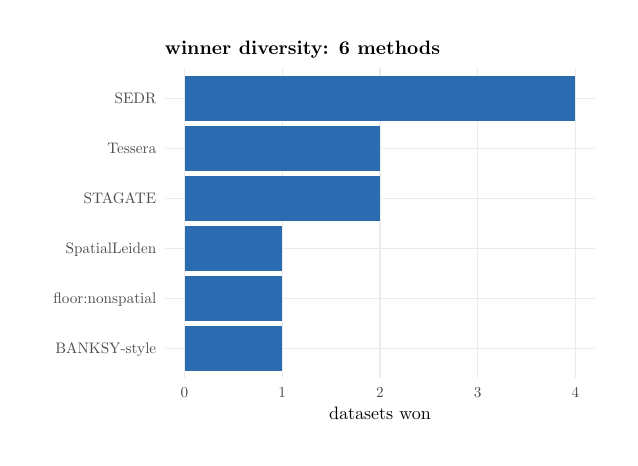
\begin{tikzpicture}[x=1pt,y=1pt]
\definecolor{fillColor}{RGB}{255,255,255}
\path[use as bounding box,fill=fillColor,fill opacity=0.00] (0,0) rectangle (210.44,148.14);
\begin{scope}
\path[clip] (  1.45,  1.84) rectangle (209.00,146.30);
\definecolor{fillColor}{RGB}{255,255,255}

\path[fill=fillColor] (  1.45,  1.84) rectangle (209.00,146.30);
\end{scope}
\begin{scope}
\path[clip] ( 49.61, 21.41) rectangle (205.00,133.43);
\definecolor{drawColor}{gray}{0.92}

\path[draw=drawColor,line width= 0.4pt,line join=round] ( 49.61, 32.25) --
	(205.00, 32.25);

\path[draw=drawColor,line width= 0.4pt,line join=round] ( 49.61, 50.32) --
	(205.00, 50.32);

\path[draw=drawColor,line width= 0.4pt,line join=round] ( 49.61, 68.38) --
	(205.00, 68.38);

\path[draw=drawColor,line width= 0.4pt,line join=round] ( 49.61, 86.45) --
	(205.00, 86.45);

\path[draw=drawColor,line width= 0.4pt,line join=round] ( 49.61,104.52) --
	(205.00,104.52);

\path[draw=drawColor,line width= 0.4pt,line join=round] ( 49.61,122.59) --
	(205.00,122.59);

\path[draw=drawColor,line width= 0.4pt,line join=round] ( 56.68, 21.41) --
	( 56.68,133.43);

\path[draw=drawColor,line width= 0.4pt,line join=round] ( 91.99, 21.41) --
	( 91.99,133.43);

\path[draw=drawColor,line width= 0.4pt,line join=round] (127.30, 21.41) --
	(127.30,133.43);

\path[draw=drawColor,line width= 0.4pt,line join=round] (162.62, 21.41) --
	(162.62,133.43);

\path[draw=drawColor,line width= 0.4pt,line join=round] (197.93, 21.41) --
	(197.93,133.43);
\definecolor{fillColor}{RGB}{43,108,176}

\path[fill=fillColor] ( 56.68, 24.12) rectangle ( 91.99, 40.38);

\path[fill=fillColor] ( 56.68, 42.19) rectangle ( 91.99, 58.45);

\path[fill=fillColor] ( 56.68,114.46) rectangle (197.93,130.72);

\path[fill=fillColor] ( 56.68, 60.25) rectangle ( 91.99, 76.51);

\path[fill=fillColor] ( 56.68, 78.32) rectangle (127.30, 94.58);

\path[fill=fillColor] ( 56.68, 96.39) rectangle (127.30,112.65);
\end{scope}
\begin{scope}
\path[clip] (  0.00,  0.00) rectangle (210.44,148.14);
\definecolor{drawColor}{gray}{0.30}

\node[text=drawColor,anchor=base east,inner sep=0pt, outer sep=0pt, scale=  0.55] at ( 46.46, 30.35) {BANKSY-style};

\node[text=drawColor,anchor=base east,inner sep=0pt, outer sep=0pt, scale=  0.55] at ( 46.46, 48.42) {floor:nonspatial};

\node[text=drawColor,anchor=base east,inner sep=0pt, outer sep=0pt, scale=  0.55] at ( 46.46, 66.49) {SpatialLeiden};

\node[text=drawColor,anchor=base east,inner sep=0pt, outer sep=0pt, scale=  0.55] at ( 46.46, 84.56) {STAGATE};

\node[text=drawColor,anchor=base east,inner sep=0pt, outer sep=0pt, scale=  0.55] at ( 46.46,102.62) {Tessera};

\node[text=drawColor,anchor=base east,inner sep=0pt, outer sep=0pt, scale=  0.55] at ( 46.46,120.69) {SEDR};
\end{scope}
\begin{scope}
\path[clip] (  0.00,  0.00) rectangle (210.44,148.14);
\definecolor{drawColor}{gray}{0.30}

\node[text=drawColor,anchor=base,inner sep=0pt, outer sep=0pt, scale=  0.55] at ( 56.68, 14.47) {0};

\node[text=drawColor,anchor=base,inner sep=0pt, outer sep=0pt, scale=  0.55] at ( 91.99, 14.47) {1};

\node[text=drawColor,anchor=base,inner sep=0pt, outer sep=0pt, scale=  0.55] at (127.30, 14.47) {2};

\node[text=drawColor,anchor=base,inner sep=0pt, outer sep=0pt, scale=  0.55] at (162.62, 14.47) {3};

\node[text=drawColor,anchor=base,inner sep=0pt, outer sep=0pt, scale=  0.55] at (197.93, 14.47) {4};
\end{scope}
\begin{scope}
\path[clip] (  0.00,  0.00) rectangle (210.44,148.14);
\definecolor{drawColor}{RGB}{0,0,0}

\node[text=drawColor,anchor=base,inner sep=0pt, outer sep=0pt, scale=  0.65] at (127.30,  6.38) {datasets won};
\end{scope}
\begin{scope}
\path[clip] (  0.00,  0.00) rectangle (210.44,148.14);
\definecolor{drawColor}{RGB}{0,0,0}

\node[text=drawColor,anchor=base west,inner sep=0pt, outer sep=0pt, scale=  0.70] at ( 49.61,138.47) {\bfseries winner diversity: 6 methods};
\end{scope}
\end{tikzpicture}
}
\caption{The law survives the author-recommended backend (real R mclust): published versus mclust-backend
advantage stays close to the diagonal for most datasets (a; a few, such as IMC, move more), and the fairer
backend shifts every method's \emph{mean} ARI by $\leq 0.016$ (b).}
\label{fig:backend}
\end{figure}

\section{A worked example: a false SOTA and a false mechanism from one dataset}\label{sec:tessera}
We close with the candidate boundary-aware method (Tessera) as one worked example of how single-dataset
evaluation can certify two claims that do not survive scrutiny: a state-of-the-art ranking, and a working
novel mechanism. We do not claim every SOTA report is false; we show, on a method we built and can fully
dissect, how both claims arise and how a multi-dataset, ablation-controlled view overturns them.

\begin{figure}[htbp]\centering
% Mechanism schematic (hand-written TikZ). Compiled with lualatex; \input directly into paper.tex.
% Replaces the README ASCII diagram: the candidate boundary-aware method, in one figure.
% Colours (tblue/tgreen/torange/tred/tgray) are defined once in paper.tex's preamble.
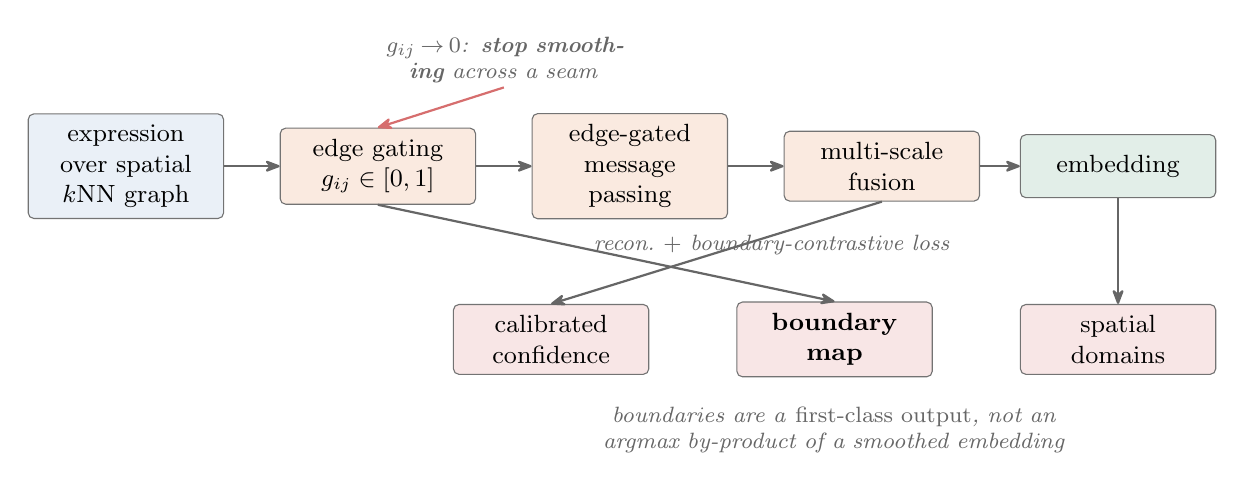
\begin{tikzpicture}[
    font=\small,
    >={Stealth[round]},
    box/.style={rounded corners=2pt, draw=black!55, fill=#1, minimum height=8mm,
                inner sep=4pt, align=center, text width=22mm},
    data/.style={box=tblue!10}, op/.style={box=torange!14}, res/.style={box=tgreen!14},
    outbox/.style={box=tred!12},
    lbl/.style={font=\footnotesize\itshape, text=black!60},
    arr/.style={->, thick, draw=black!60},
]

% ---------- main forward path ----------
\node[data] (expr)  at (0,0)    {expression\\over spatial\\$k$NN graph};
\node[op]   (gate)  at (3.2,0)  {edge gating\\$g_{ij}\!\in\![0,1]$};
\node[op]   (mp)    at (6.4,0)  {edge-gated\\message passing};
\node[op]   (fuse)  at (9.6,0)  {multi-scale\\fusion};
\node[res]  (emb)   at (12.6,0) {embedding};

\draw[arr] (expr) -- (gate);
\draw[arr] (gate) -- (mp);
\draw[arr] (mp)   -- (fuse);
\draw[arr] (fuse) -- (emb);

% the anti-over-smoothing annotation on the gate
\node[lbl, align=center, text width=34mm] at (4.8,1.35)
  {$g_{ij}\!\rightarrow\!0$: \textbf{stop smoothing} across a seam};
\draw[->, draw=tred!70, thick] (4.8,1.0) -- (gate.north);

% ---------- three first-class outputs ----------
\node[outbox] (dom)  at (12.6,-2.2) {spatial\\domains};
\node[outbox] (bmap) at (9.0,-2.2)  {\textbf{boundary}\\\textbf{map}};
\node[outbox] (conf) at (5.4,-2.2)  {calibrated\\confidence};

\draw[arr] (emb)  -- (dom);
\draw[arr] (gate.south) -- (bmap.north);
\draw[arr] (fuse.south) -- (conf.north);

\node[lbl, align=center, text width=90mm] at (9.0,-3.35)
  {boundaries are a \emph{first-class output}, not an argmax by-product of a smoothed embedding};

% loss tag between the forward path and the outputs
\node[lbl] at (8.2,-1.0) {recon.\ $+$ boundary-contrastive loss};

\end{tikzpicture}

\caption{The candidate method (Tessera) in one diagram. A learned per-edge gate $g_{ij}$ down-weights
message passing across tissue seams (anti-over-smoothing); multi-scale fusion combines the gated
representations into an embedding that is clustered into domains, with the boundary map and a calibrated
confidence as explicit outputs. The component ablation (Fig.~\ref{fig:ablation}) tests whether each
part contributes.}
\label{fig:arch}
\end{figure}

\paragraph{A single favourable dataset certifies a false SOTA.} On osmFISH the method ranks first (ARI $0.438$,
$+0.196$ over the non-spatial floor), a publishable state-of-the-art claim from a single ARI table.
Across the full 11-dataset panel, however, it is a backend-robust generalist, not a winner: its rank
swings from $1$ to $8$ (Fig.~\ref{fig:profile}), its one win (osmFISH) is by only $0.005$ ARI over the next
spatial method, and on IMC it trails the best method by $0.39$ ARI. On the other contiguous task, MERFISH,
the top spot is a seed-level tie it does not hold (the winner flips SpaceFlow, Tessera, SpaceFlow across
three runs). No dataset has it uniquely best; the most backend-stable embedding ($\Delta$ARI $0.036$) is its
real, and far more modest, property.

\paragraph{The headline mechanism does not drive the gain.} The method's advertised contribution is
anti-over-smoothing through the learned edge gate (Fig.~\ref{fig:arch}). A component ablation on the two
datasets where it is competitive (Fig.~\ref{fig:ablation}) refutes that account: only the
boundary-contrastive loss matters. Removing it collapses ARI $0.45\!\to\!0.17/0.20$, back to a
plain graph-autoencoder backbone, while the named edge gate and multi-scale fusion are neutral-to-harmful
($-0.01$ to $-0.03$). The full model beats the backbone by $+0.29/+0.23$, but that entire gain is the
generic contrastive objective, not the mechanism the method is named for.

\begin{figure}[htbp]\centering
\resizebox{0.92\linewidth}{!}{% !TEX encoding = UTF-8 Unicode
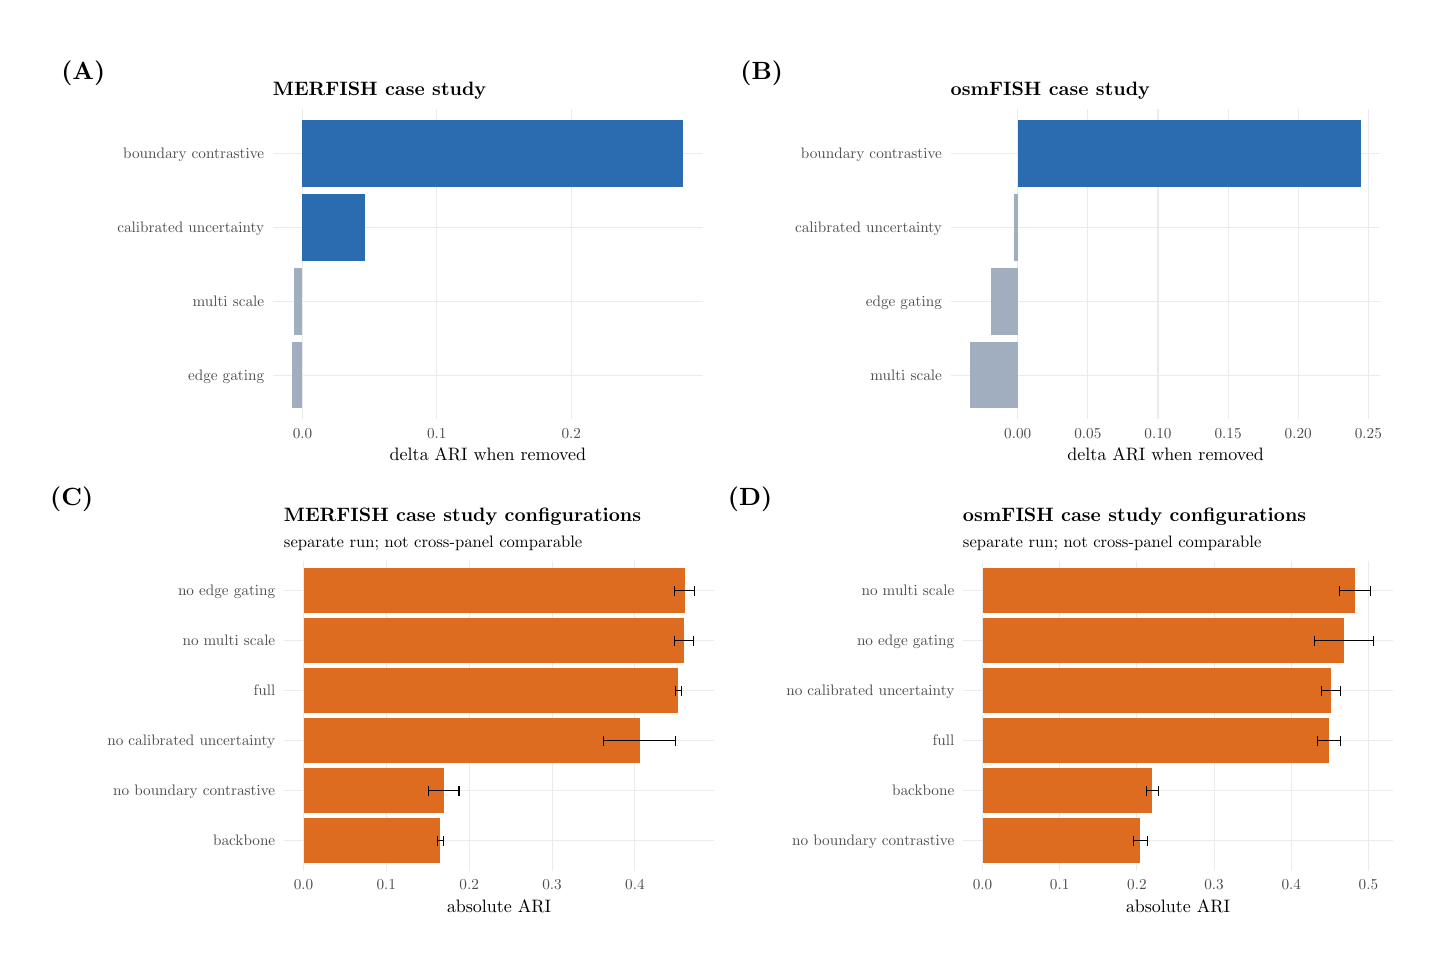
\begin{tikzpicture}[x=1pt,y=1pt]
\definecolor{fillColor}{RGB}{255,255,255}
\path[use as bounding box,fill=fillColor,fill opacity=0.00] (0,0) rectangle (501.28,328.16);
\begin{scope}
\path[clip] (  0.00,  0.00) rectangle (501.28,328.16);
\definecolor{drawColor}{RGB}{255,255,255}
\definecolor{fillColor}{RGB}{255,255,255}

\path[draw=drawColor,line width= 0.6pt,line join=round,line cap=round,fill=fillColor] (  0.00,  0.00) rectangle (501.28,328.16);
\end{scope}
\begin{scope}
\path[clip] (  5.50,164.08) rectangle (250.64,322.66);
\definecolor{drawColor}{RGB}{255,255,255}
\definecolor{fillColor}{RGB}{255,255,255}

\path[draw=drawColor,line width= 0.6pt,line join=round,line cap=round,fill=fillColor] (  5.50,164.08) rectangle (250.64,322.66);
\end{scope}
\begin{scope}
\path[clip] (250.64,164.08) rectangle (495.78,322.66);
\definecolor{drawColor}{RGB}{255,255,255}
\definecolor{fillColor}{RGB}{255,255,255}

\path[draw=drawColor,line width= 0.6pt,line join=round,line cap=round,fill=fillColor] (250.64,164.08) rectangle (495.78,322.66);
\end{scope}
\begin{scope}
\path[clip] (  8.16,167.04) rectangle (247.98,319.70);
\definecolor{fillColor}{RGB}{255,255,255}

\path[fill=fillColor] (  8.16,167.04) rectangle (247.98,319.70);
\end{scope}
\begin{scope}
\path[clip] ( 88.60,186.61) rectangle (243.98,298.63);
\definecolor{drawColor}{gray}{0.92}

\path[draw=drawColor,line width= 0.4pt,line join=round] ( 88.60,202.61) --
	(243.98,202.61);

\path[draw=drawColor,line width= 0.4pt,line join=round] ( 88.60,229.28) --
	(243.98,229.28);

\path[draw=drawColor,line width= 0.4pt,line join=round] ( 88.60,255.95) --
	(243.98,255.95);

\path[draw=drawColor,line width= 0.4pt,line join=round] ( 88.60,282.62) --
	(243.98,282.62);

\path[draw=drawColor,line width= 0.4pt,line join=round] ( 99.30,186.61) --
	( 99.30,298.63);

\path[draw=drawColor,line width= 0.4pt,line join=round] (147.86,186.61) --
	(147.86,298.63);

\path[draw=drawColor,line width= 0.4pt,line join=round] (196.42,186.61) --
	(196.42,298.63);
\definecolor{fillColor}{RGB}{43,108,176}

\path[fill=fillColor] ( 99.30,270.62) rectangle (236.92,294.62);

\path[fill=fillColor] ( 99.30,243.95) rectangle (121.98,267.95);
\definecolor{fillColor}{RGB}{160,174,192}

\path[fill=fillColor] ( 95.66,190.61) rectangle ( 99.30,214.61);

\path[fill=fillColor] ( 96.25,217.28) rectangle ( 99.30,241.28);
\end{scope}
\begin{scope}
\path[clip] (  0.00,  0.00) rectangle (501.28,328.16);
\definecolor{drawColor}{gray}{0.30}

\node[text=drawColor,anchor=base east,inner sep=0pt, outer sep=0pt, scale=  0.55] at ( 85.45,200.72) {edge gating};

\node[text=drawColor,anchor=base east,inner sep=0pt, outer sep=0pt, scale=  0.55] at ( 85.45,227.39) {multi scale};

\node[text=drawColor,anchor=base east,inner sep=0pt, outer sep=0pt, scale=  0.55] at ( 85.45,254.06) {calibrated uncertainty};

\node[text=drawColor,anchor=base east,inner sep=0pt, outer sep=0pt, scale=  0.55] at ( 85.45,280.73) {boundary contrastive};
\end{scope}
\begin{scope}
\path[clip] (  0.00,  0.00) rectangle (501.28,328.16);
\definecolor{drawColor}{gray}{0.30}

\node[text=drawColor,anchor=base,inner sep=0pt, outer sep=0pt, scale=  0.55] at ( 99.30,179.67) {0.0};

\node[text=drawColor,anchor=base,inner sep=0pt, outer sep=0pt, scale=  0.55] at (147.86,179.67) {0.1};

\node[text=drawColor,anchor=base,inner sep=0pt, outer sep=0pt, scale=  0.55] at (196.42,179.67) {0.2};
\end{scope}
\begin{scope}
\path[clip] (  0.00,  0.00) rectangle (501.28,328.16);
\definecolor{drawColor}{RGB}{0,0,0}

\node[text=drawColor,anchor=base,inner sep=0pt, outer sep=0pt, scale=  0.65] at (166.29,171.58) {delta ARI when removed};
\end{scope}
\begin{scope}
\path[clip] (  0.00,  0.00) rectangle (501.28,328.16);
\definecolor{drawColor}{RGB}{0,0,0}

\node[text=drawColor,anchor=base west,inner sep=0pt, outer sep=0pt, scale=  0.70] at ( 88.60,303.67) {\bfseries MERFISH case study};
\end{scope}
\begin{scope}
\path[clip] (  0.00,  0.00) rectangle (501.28,328.16);
\definecolor{drawColor}{RGB}{0,0,0}

\node[text=drawColor,anchor=base,inner sep=0pt, outer sep=0pt, scale=  0.90] at ( 20.10,309.50) {\bfseries (A)};
\end{scope}
\begin{scope}
\path[clip] (253.53,167.04) rectangle (492.89,319.70);
\definecolor{fillColor}{RGB}{255,255,255}

\path[fill=fillColor] (253.53,167.04) rectangle (492.89,319.70);
\end{scope}
\begin{scope}
\path[clip] (333.51,186.61) rectangle (488.89,298.63);
\definecolor{drawColor}{gray}{0.92}

\path[draw=drawColor,line width= 0.4pt,line join=round] (333.51,202.61) --
	(488.89,202.61);

\path[draw=drawColor,line width= 0.4pt,line join=round] (333.51,229.28) --
	(488.89,229.28);

\path[draw=drawColor,line width= 0.4pt,line join=round] (333.51,255.95) --
	(488.89,255.95);

\path[draw=drawColor,line width= 0.4pt,line join=round] (333.51,282.62) --
	(488.89,282.62);

\path[draw=drawColor,line width= 0.4pt,line join=round] (357.75,186.61) --
	(357.75,298.63);

\path[draw=drawColor,line width= 0.4pt,line join=round] (383.10,186.61) --
	(383.10,298.63);

\path[draw=drawColor,line width= 0.4pt,line join=round] (408.44,186.61) --
	(408.44,298.63);

\path[draw=drawColor,line width= 0.4pt,line join=round] (433.78,186.61) --
	(433.78,298.63);

\path[draw=drawColor,line width= 0.4pt,line join=round] (459.12,186.61) --
	(459.12,298.63);

\path[draw=drawColor,line width= 0.4pt,line join=round] (484.46,186.61) --
	(484.46,298.63);
\definecolor{fillColor}{RGB}{43,108,176}

\path[fill=fillColor] (357.75,270.62) rectangle (481.83,294.62);
\definecolor{fillColor}{RGB}{160,174,192}

\path[fill=fillColor] (356.54,243.95) rectangle (357.75,267.95);

\path[fill=fillColor] (348.07,217.28) rectangle (357.75,241.28);

\path[fill=fillColor] (340.57,190.61) rectangle (357.75,214.61);
\end{scope}
\begin{scope}
\path[clip] (  0.00,  0.00) rectangle (501.28,328.16);
\definecolor{drawColor}{gray}{0.30}

\node[text=drawColor,anchor=base east,inner sep=0pt, outer sep=0pt, scale=  0.55] at (330.36,200.72) {multi scale};

\node[text=drawColor,anchor=base east,inner sep=0pt, outer sep=0pt, scale=  0.55] at (330.36,227.39) {edge gating};

\node[text=drawColor,anchor=base east,inner sep=0pt, outer sep=0pt, scale=  0.55] at (330.36,254.06) {calibrated uncertainty};

\node[text=drawColor,anchor=base east,inner sep=0pt, outer sep=0pt, scale=  0.55] at (330.36,280.73) {boundary contrastive};
\end{scope}
\begin{scope}
\path[clip] (  0.00,  0.00) rectangle (501.28,328.16);
\definecolor{drawColor}{gray}{0.30}

\node[text=drawColor,anchor=base,inner sep=0pt, outer sep=0pt, scale=  0.55] at (357.75,179.67) {0.00};

\node[text=drawColor,anchor=base,inner sep=0pt, outer sep=0pt, scale=  0.55] at (383.10,179.67) {0.05};

\node[text=drawColor,anchor=base,inner sep=0pt, outer sep=0pt, scale=  0.55] at (408.44,179.67) {0.10};

\node[text=drawColor,anchor=base,inner sep=0pt, outer sep=0pt, scale=  0.55] at (433.78,179.67) {0.15};

\node[text=drawColor,anchor=base,inner sep=0pt, outer sep=0pt, scale=  0.55] at (459.12,179.67) {0.20};

\node[text=drawColor,anchor=base,inner sep=0pt, outer sep=0pt, scale=  0.55] at (484.46,179.67) {0.25};
\end{scope}
\begin{scope}
\path[clip] (  0.00,  0.00) rectangle (501.28,328.16);
\definecolor{drawColor}{RGB}{0,0,0}

\node[text=drawColor,anchor=base,inner sep=0pt, outer sep=0pt, scale=  0.65] at (411.20,171.58) {delta ARI when removed};
\end{scope}
\begin{scope}
\path[clip] (  0.00,  0.00) rectangle (501.28,328.16);
\definecolor{drawColor}{RGB}{0,0,0}

\node[text=drawColor,anchor=base west,inner sep=0pt, outer sep=0pt, scale=  0.70] at (333.51,303.67) {\bfseries osmFISH case study};
\end{scope}
\begin{scope}
\path[clip] (  0.00,  0.00) rectangle (501.28,328.16);
\definecolor{drawColor}{RGB}{0,0,0}

\node[text=drawColor,anchor=base,inner sep=0pt, outer sep=0pt, scale=  0.90] at (265.24,309.50) {\bfseries (B)};
\end{scope}
\begin{scope}
\path[clip] (  5.50,  5.50) rectangle (250.64,164.08);
\definecolor{drawColor}{RGB}{255,255,255}
\definecolor{fillColor}{RGB}{255,255,255}

\path[draw=drawColor,line width= 0.6pt,line join=round,line cap=round,fill=fillColor] (  5.50,  5.50) rectangle (250.64,164.08);
\end{scope}
\begin{scope}
\path[clip] (250.64,  5.50) rectangle (495.78,164.08);
\definecolor{drawColor}{RGB}{255,255,255}
\definecolor{fillColor}{RGB}{255,255,255}

\path[draw=drawColor,line width= 0.6pt,line join=round,line cap=round,fill=fillColor] (250.64,  5.50) rectangle (495.78,164.08);
\end{scope}
\begin{scope}
\path[clip] (  4.15,  3.98) rectangle (251.99,165.60);
\definecolor{fillColor}{RGB}{255,255,255}

\path[fill=fillColor] (  4.15,  3.98) rectangle (251.99,165.60);
\end{scope}
\begin{scope}
\path[clip] ( 92.61, 23.55) rectangle (247.99,135.57);
\definecolor{drawColor}{gray}{0.92}

\path[draw=drawColor,line width= 0.4pt,line join=round] ( 92.61, 34.39) --
	(247.99, 34.39);

\path[draw=drawColor,line width= 0.4pt,line join=round] ( 92.61, 52.46) --
	(247.99, 52.46);

\path[draw=drawColor,line width= 0.4pt,line join=round] ( 92.61, 70.53) --
	(247.99, 70.53);

\path[draw=drawColor,line width= 0.4pt,line join=round] ( 92.61, 88.59) --
	(247.99, 88.59);

\path[draw=drawColor,line width= 0.4pt,line join=round] ( 92.61,106.66) --
	(247.99,106.66);

\path[draw=drawColor,line width= 0.4pt,line join=round] ( 92.61,124.73) --
	(247.99,124.73);

\path[draw=drawColor,line width= 0.4pt,line join=round] ( 99.67, 23.55) --
	( 99.67,135.57);

\path[draw=drawColor,line width= 0.4pt,line join=round] (129.61, 23.55) --
	(129.61,135.57);

\path[draw=drawColor,line width= 0.4pt,line join=round] (159.55, 23.55) --
	(159.55,135.57);

\path[draw=drawColor,line width= 0.4pt,line join=round] (189.49, 23.55) --
	(189.49,135.57);

\path[draw=drawColor,line width= 0.4pt,line join=round] (219.43, 23.55) --
	(219.43,135.57);
\definecolor{fillColor}{RGB}{221,107,32}

\path[fill=fillColor] ( 99.67, 80.46) rectangle (235.15, 96.72);

\path[fill=fillColor] ( 99.67,116.60) rectangle (237.40,132.86);

\path[fill=fillColor] ( 99.67, 98.53) rectangle (237.04,114.79);

\path[fill=fillColor] ( 99.67, 44.33) rectangle (150.30, 60.59);

\path[fill=fillColor] ( 99.67, 62.39) rectangle (221.17, 78.66);

\path[fill=fillColor] ( 99.67, 26.26) rectangle (149.16, 42.52);
\definecolor{drawColor}{RGB}{0,0,0}

\path[draw=drawColor,line width= 0.4pt,line join=round] (236.20, 86.79) --
	(236.20, 90.40);

\path[draw=drawColor,line width= 0.4pt,line join=round] (236.20, 88.59) --
	(234.10, 88.59);

\path[draw=drawColor,line width= 0.4pt,line join=round] (234.10, 86.79) --
	(234.10, 90.40);

\path[draw=drawColor,line width= 0.4pt,line join=round] (240.93,122.92) --
	(240.93,126.53);

\path[draw=drawColor,line width= 0.4pt,line join=round] (240.93,124.73) --
	(233.86,124.73);

\path[draw=drawColor,line width= 0.4pt,line join=round] (233.86,122.92) --
	(233.86,126.53);

\path[draw=drawColor,line width= 0.4pt,line join=round] (240.45,104.85) --
	(240.45,108.47);

\path[draw=drawColor,line width= 0.4pt,line join=round] (240.45,106.66) --
	(233.62,106.66);

\path[draw=drawColor,line width= 0.4pt,line join=round] (233.62,104.85) --
	(233.62,108.47);

\path[draw=drawColor,line width= 0.4pt,line join=round] (155.84, 50.65) --
	(155.84, 54.26);

\path[draw=drawColor,line width= 0.4pt,line join=round] (155.84, 52.46) --
	(144.76, 52.46);

\path[draw=drawColor,line width= 0.4pt,line join=round] (144.76, 50.65) --
	(144.76, 54.26);

\path[draw=drawColor,line width= 0.4pt,line join=round] (234.10, 68.72) --
	(234.10, 72.33);

\path[draw=drawColor,line width= 0.4pt,line join=round] (234.10, 70.53) --
	(208.23, 70.53);

\path[draw=drawColor,line width= 0.4pt,line join=round] (208.23, 68.72) --
	(208.23, 72.33);

\path[draw=drawColor,line width= 0.4pt,line join=round] (150.12, 32.58) --
	(150.12, 36.20);

\path[draw=drawColor,line width= 0.4pt,line join=round] (150.12, 34.39) --
	(148.21, 34.39);

\path[draw=drawColor,line width= 0.4pt,line join=round] (148.21, 32.58) --
	(148.21, 36.20);
\end{scope}
\begin{scope}
\path[clip] (  0.00,  0.00) rectangle (501.28,328.16);
\definecolor{drawColor}{gray}{0.30}

\node[text=drawColor,anchor=base east,inner sep=0pt, outer sep=0pt, scale=  0.55] at ( 89.46, 32.50) {backbone};

\node[text=drawColor,anchor=base east,inner sep=0pt, outer sep=0pt, scale=  0.55] at ( 89.46, 50.56) {no boundary contrastive};

\node[text=drawColor,anchor=base east,inner sep=0pt, outer sep=0pt, scale=  0.55] at ( 89.46, 68.63) {no calibrated uncertainty};

\node[text=drawColor,anchor=base east,inner sep=0pt, outer sep=0pt, scale=  0.55] at ( 89.46, 86.70) {full};

\node[text=drawColor,anchor=base east,inner sep=0pt, outer sep=0pt, scale=  0.55] at ( 89.46,104.77) {no multi scale};

\node[text=drawColor,anchor=base east,inner sep=0pt, outer sep=0pt, scale=  0.55] at ( 89.46,122.83) {no edge gating};
\end{scope}
\begin{scope}
\path[clip] (  0.00,  0.00) rectangle (501.28,328.16);
\definecolor{drawColor}{gray}{0.30}

\node[text=drawColor,anchor=base,inner sep=0pt, outer sep=0pt, scale=  0.55] at ( 99.67, 16.61) {0.0};

\node[text=drawColor,anchor=base,inner sep=0pt, outer sep=0pt, scale=  0.55] at (129.61, 16.61) {0.1};

\node[text=drawColor,anchor=base,inner sep=0pt, outer sep=0pt, scale=  0.55] at (159.55, 16.61) {0.2};

\node[text=drawColor,anchor=base,inner sep=0pt, outer sep=0pt, scale=  0.55] at (189.49, 16.61) {0.3};

\node[text=drawColor,anchor=base,inner sep=0pt, outer sep=0pt, scale=  0.55] at (219.43, 16.61) {0.4};
\end{scope}
\begin{scope}
\path[clip] (  0.00,  0.00) rectangle (501.28,328.16);
\definecolor{drawColor}{RGB}{0,0,0}

\node[text=drawColor,anchor=base,inner sep=0pt, outer sep=0pt, scale=  0.65] at (170.30,  8.52) {absolute ARI};
\end{scope}
\begin{scope}
\path[clip] (  0.00,  0.00) rectangle (501.28,328.16);
\definecolor{drawColor}{RGB}{0,0,0}

\node[text=drawColor,anchor=base west,inner sep=0pt, outer sep=0pt, scale=  0.60] at ( 92.61,140.39) {separate run; not cross-panel comparable};
\end{scope}
\begin{scope}
\path[clip] (  0.00,  0.00) rectangle (501.28,328.16);
\definecolor{drawColor}{RGB}{0,0,0}

\node[text=drawColor,anchor=base west,inner sep=0pt, outer sep=0pt, scale=  0.70] at ( 92.61,149.57) {\bfseries MERFISH case study configurations};
\end{scope}
\begin{scope}
\path[clip] (  0.00,  0.00) rectangle (501.28,328.16);
\definecolor{drawColor}{RGB}{0,0,0}

\node[text=drawColor,anchor=base,inner sep=0pt, outer sep=0pt, scale=  0.90] at ( 15.91,155.40) {\bfseries (C)};
\end{scope}
\begin{scope}
\path[clip] (249.06,  3.98) rectangle (497.36,165.60);
\definecolor{fillColor}{RGB}{255,255,255}

\path[fill=fillColor] (249.06,  3.98) rectangle (497.36,165.60);
\end{scope}
\begin{scope}
\path[clip] (337.98, 23.55) rectangle (493.36,135.57);
\definecolor{drawColor}{gray}{0.92}

\path[draw=drawColor,line width= 0.4pt,line join=round] (337.98, 34.39) --
	(493.36, 34.39);

\path[draw=drawColor,line width= 0.4pt,line join=round] (337.98, 52.46) --
	(493.36, 52.46);

\path[draw=drawColor,line width= 0.4pt,line join=round] (337.98, 70.53) --
	(493.36, 70.53);

\path[draw=drawColor,line width= 0.4pt,line join=round] (337.98, 88.59) --
	(493.36, 88.59);

\path[draw=drawColor,line width= 0.4pt,line join=round] (337.98,106.66) --
	(493.36,106.66);

\path[draw=drawColor,line width= 0.4pt,line join=round] (337.98,124.73) --
	(493.36,124.73);

\path[draw=drawColor,line width= 0.4pt,line join=round] (345.05, 23.55) --
	(345.05,135.57);

\path[draw=drawColor,line width= 0.4pt,line join=round] (372.93, 23.55) --
	(372.93,135.57);

\path[draw=drawColor,line width= 0.4pt,line join=round] (400.82, 23.55) --
	(400.82,135.57);

\path[draw=drawColor,line width= 0.4pt,line join=round] (428.71, 23.55) --
	(428.71,135.57);

\path[draw=drawColor,line width= 0.4pt,line join=round] (456.60, 23.55) --
	(456.60,135.57);

\path[draw=drawColor,line width= 0.4pt,line join=round] (484.49, 23.55) --
	(484.49,135.57);
\definecolor{fillColor}{RGB}{221,107,32}

\path[fill=fillColor] (345.05, 62.39) rectangle (470.26, 78.66);

\path[fill=fillColor] (345.05, 98.53) rectangle (475.59,114.79);

\path[fill=fillColor] (345.05,116.60) rectangle (479.72,132.86);

\path[fill=fillColor] (345.05, 26.26) rectangle (401.99, 42.52);

\path[fill=fillColor] (345.05, 80.46) rectangle (470.93, 96.72);

\path[fill=fillColor] (345.05, 44.33) rectangle (406.34, 60.59);
\definecolor{drawColor}{RGB}{0,0,0}

\path[draw=drawColor,line width= 0.4pt,line join=round] (474.45, 68.72) --
	(474.45, 72.33);

\path[draw=drawColor,line width= 0.4pt,line join=round] (474.45, 70.53) --
	(466.08, 70.53);

\path[draw=drawColor,line width= 0.4pt,line join=round] (466.08, 68.72) --
	(466.08, 72.33);

\path[draw=drawColor,line width= 0.4pt,line join=round] (486.30,104.85) --
	(486.30,108.47);

\path[draw=drawColor,line width= 0.4pt,line join=round] (486.30,106.66) --
	(464.88,106.66);

\path[draw=drawColor,line width= 0.4pt,line join=round] (464.88,104.85) --
	(464.88,108.47);

\path[draw=drawColor,line width= 0.4pt,line join=round] (485.32,122.92) --
	(485.32,126.53);

\path[draw=drawColor,line width= 0.4pt,line join=round] (485.32,124.73) --
	(474.11,124.73);

\path[draw=drawColor,line width= 0.4pt,line join=round] (474.11,122.92) --
	(474.11,126.53);

\path[draw=drawColor,line width= 0.4pt,line join=round] (404.53, 32.58) --
	(404.53, 36.20);

\path[draw=drawColor,line width= 0.4pt,line join=round] (404.53, 34.39) --
	(399.46, 34.39);

\path[draw=drawColor,line width= 0.4pt,line join=round] (399.46, 32.58) --
	(399.46, 36.20);

\path[draw=drawColor,line width= 0.4pt,line join=round] (474.48, 86.79) --
	(474.48, 90.40);

\path[draw=drawColor,line width= 0.4pt,line join=round] (474.48, 88.59) --
	(467.39, 88.59);

\path[draw=drawColor,line width= 0.4pt,line join=round] (467.39, 86.79) --
	(467.39, 90.40);

\path[draw=drawColor,line width= 0.4pt,line join=round] (408.46, 50.65) --
	(408.46, 54.26);

\path[draw=drawColor,line width= 0.4pt,line join=round] (408.46, 52.46) --
	(404.22, 52.46);

\path[draw=drawColor,line width= 0.4pt,line join=round] (404.22, 50.65) --
	(404.22, 54.26);
\end{scope}
\begin{scope}
\path[clip] (  0.00,  0.00) rectangle (501.28,328.16);
\definecolor{drawColor}{gray}{0.30}

\node[text=drawColor,anchor=base east,inner sep=0pt, outer sep=0pt, scale=  0.55] at (334.83, 32.50) {no boundary contrastive};

\node[text=drawColor,anchor=base east,inner sep=0pt, outer sep=0pt, scale=  0.55] at (334.83, 50.56) {backbone};

\node[text=drawColor,anchor=base east,inner sep=0pt, outer sep=0pt, scale=  0.55] at (334.83, 68.63) {full};

\node[text=drawColor,anchor=base east,inner sep=0pt, outer sep=0pt, scale=  0.55] at (334.83, 86.70) {no calibrated uncertainty};

\node[text=drawColor,anchor=base east,inner sep=0pt, outer sep=0pt, scale=  0.55] at (334.83,104.77) {no edge gating};

\node[text=drawColor,anchor=base east,inner sep=0pt, outer sep=0pt, scale=  0.55] at (334.83,122.83) {no multi scale};
\end{scope}
\begin{scope}
\path[clip] (  0.00,  0.00) rectangle (501.28,328.16);
\definecolor{drawColor}{gray}{0.30}

\node[text=drawColor,anchor=base,inner sep=0pt, outer sep=0pt, scale=  0.55] at (345.05, 16.61) {0.0};

\node[text=drawColor,anchor=base,inner sep=0pt, outer sep=0pt, scale=  0.55] at (372.93, 16.61) {0.1};

\node[text=drawColor,anchor=base,inner sep=0pt, outer sep=0pt, scale=  0.55] at (400.82, 16.61) {0.2};

\node[text=drawColor,anchor=base,inner sep=0pt, outer sep=0pt, scale=  0.55] at (428.71, 16.61) {0.3};

\node[text=drawColor,anchor=base,inner sep=0pt, outer sep=0pt, scale=  0.55] at (456.60, 16.61) {0.4};

\node[text=drawColor,anchor=base,inner sep=0pt, outer sep=0pt, scale=  0.55] at (484.49, 16.61) {0.5};
\end{scope}
\begin{scope}
\path[clip] (  0.00,  0.00) rectangle (501.28,328.16);
\definecolor{drawColor}{RGB}{0,0,0}

\node[text=drawColor,anchor=base,inner sep=0pt, outer sep=0pt, scale=  0.65] at (415.67,  8.52) {absolute ARI};
\end{scope}
\begin{scope}
\path[clip] (  0.00,  0.00) rectangle (501.28,328.16);
\definecolor{drawColor}{RGB}{0,0,0}

\node[text=drawColor,anchor=base west,inner sep=0pt, outer sep=0pt, scale=  0.60] at (337.98,140.39) {separate run; not cross-panel comparable};
\end{scope}
\begin{scope}
\path[clip] (  0.00,  0.00) rectangle (501.28,328.16);
\definecolor{drawColor}{RGB}{0,0,0}

\node[text=drawColor,anchor=base west,inner sep=0pt, outer sep=0pt, scale=  0.70] at (337.98,149.57) {\bfseries osmFISH case study configurations};
\end{scope}
\begin{scope}
\path[clip] (  0.00,  0.00) rectangle (501.28,328.16);
\definecolor{drawColor}{RGB}{0,0,0}

\node[text=drawColor,anchor=base,inner sep=0pt, outer sep=0pt, scale=  0.90] at (261.05,155.40) {\bfseries (D)};
\end{scope}
\end{tikzpicture}
}
\caption{Component ablation of the candidate method on the two datasets where it is competitive (3 seeds):
the ARI drop when each component is removed (positive $=$ the component contributes). Only the
boundary-contrastive loss matters; the headline anti-over-smoothing edge gate and multi-scale
fusion are neutral-to-harmful, so the model's gain over a plain backbone is the contrastive loss alone.}
\label{fig:ablation}
\end{figure}

\paragraph{The verdict.} Single-dataset evaluation would have certified two false positives here: a
state-of-the-art ranking and a working new mechanism. The full panel and the ablation overturn both. This
is the failure mode the predictive law pre-empts: decide whether a spatial prior helps at all before
crediting any one method, or any one of its components, for the gain.

\section{Discussion}
The unit of progress in spatial-domain detection should shift from ``a better method'' to ``a better
understanding of when spatial priors help''. Our law turns the discouraging ``no universal SOTA'' finding
into an actionable, label-free check made before committing: estimate the spatial-coherence gain on the
unlabelled data; if it is low, a non-spatial clusterer is both floor and ceiling and spatial smoothing can
actively hurt (this direction is demonstrated causally in the synthetic manipulation of \S\ref{sec:causal},
where the advantage falls to $-0.33$ to $-0.34$; on the real low-contiguity datasets in our panel the effect
is present but at seed-level magnitude, spatial advantage $-0.005$ on seqFISH and Open-ST and $+0.008$ to
$+0.024$ on Slide-seqV2, MIBI-TOF, and CODEX, Table~\ref{tab:perdataset}); if it is
high, a spatial method is warranted, though which one is within seed noise. The inverted
profile of SpatialLeiden, and the fact that a popular deep method (SpaGCN) wins only a single scattered
dataset, both reinforce that method--task fit, not method identity, is what determines performance.

Because the relationship is causal, not merely correlational, and does not stand in for cluster count,
dimensionality, or modality, it can be used to choose a method in advance rather than to rationalise a
result after the fact. Removing the labels costs significance but keeps a positive predictor; broadening to
noisier tasks shrinks the correlation. Neither overturns the rule.

\section{Limitations}\label{sec:limitations}
\paragraph{Sample size and panel diversity.} The headline rests on $n{=}11$ technologically diverse,
de-duplicated datasets; broadening to three additional cell-type cancer datasets ($n{=}14$) attenuates the
correlation from $+0.72$ to $+0.56$ ($p=0.038$), so $+0.72$ is a diverse-panel upper estimate, not a
constant, and high-contiguity domain-GT datasets remain scarce.

\paragraph{Does continuous contiguity beat a coarse GT-type label?} A cheaper alternative to measuring
contiguity would be a binary label read straight off Table~\ref{tab:data}'s GT-type column: structural
ground truth (domain/region/layer/tumour) versus identity-based ground truth (cell type/niche/annotation/
cluster). On the same 11-dataset panel this coarse indicator correlates with spatial-prior advantage at
$\rho{=}0.58$ ($p=0.062$, point-biserial $r=0.52$, $p=0.099$) -- weaker and no longer significant at
$\alpha{=}0.05$, versus $\rho{=}0.72$ ($p=0.012$) for continuous contiguity. The gap is driven by
Slide-seqV2 (region GT, measured contiguity only 0.274) and IMC (cell-type GT, measured contiguity 0.630):
both are exceptions the categorical split misclassifies, because GT-type name is only a weak proxy for how
spatially contiguous the labels actually are on a given tissue. Continuous, data-measured contiguity is
therefore not redundant with a coarser categorical predictor built from the same metadata
(\texttt{experiments/gt\_type\_vs\_contiguity.py}).

\paragraph{Multiple comparisons and influence.} The headline $p=0.012$ is uncorrected and the estimate is
fragile to its small sample: it survives a Bonferroni correction over the three primary tests ($p=0.035$)
but not over the wider family of seven predictor--advantage correlations ($p=0.082$), and dropping the
single most influential dataset (MERFISH) lowers $\rho$ to $0.63$ (jackknife range $[0.63,0.75]$). Only the
advantage correlation is significant; the method-specific rank correlations are not. The out-of-sample
decision rule is real but marginal at $n{=}11$ ($p=0.06$), and the label-free \texttt{coh\_gain} proxy is
directional only: after correcting for its selection among six candidate proxies it is not significant
(search-corrected $p=0.28$; uncorrected $p=0.079$), so the causal synthetic sweep, not the proxy, carries the
weight of the label-free claim. The primary family of
three tests comprises the correlations against the study's actual predictive targets reported in
Table~\ref{tab:law} (contiguity vs.\ spatial-prior advantage, vs.\ Tessera rank, vs.\ SpaceFlow rank); the
wider family of seven additionally includes confound-marginal
correlations (cluster count, dimensionality, modality) and two label-free proxy validations (Moran's $I$,
raw coherence) computed for different diagnostic purposes, not repeated tests of the same hypothesis
(\texttt{experiments/robustness\_audit.py}).

\paragraph{Partly definitional direction.} The advantage we predict and the contiguity predictor are both
read off the same spatial $k$NN structure on the same labels. On this panel the neighbour-mean smoother is
never the winning spatial method, so the advantage never depends on it specifically; but every spatial
method here, learned graph encoders and a neighbour-augmentation method alike, is built on that same
$k$NN structure, so ``spatial methods help when the labels are spatially contiguous'' is closer to a
calibration than a discovery. What is genuinely empirical is \emph{how much} contiguity is needed before a
prior pays off, together with the out-of-sample and label-free results above. The conclusion has already
changed twice as the panel grew; it is the current best estimate, not a final word.

\paragraph{Baseline tuning and metrics.} SpaGCN is run with a kmeans initialisation (its native louvain
path is blocked by the environment) and so its absolute level is understated; GraphST receives the
recommended R mclust backend on the datasets where it runs (size-gated to $\leq$8k cells) but not its full
native preprocessing/refinement tuning, so its absolute level is a lower bound. Because GraphST anchors the
low end of Table~\ref{tab:backend}, the headline ``backend-shift equals between-method spread'' framing of
\S\ref{sec:confound} depends on retaining this under-tuned baseline: dropping GraphST shrinks the spread
from 0.203 to 0.150, below the largest single-backend shift. SpaceFlow additionally
receives its own native normalise/log/HVG/PCA pipeline rather than the shared scaled expression matrix used
by the graph methods -- a defensible per-method choice but a variable not held fixed across methods, and
SpaceFlow drives part of the headline correlation (MERFISH winner, Table~\ref{tab:perdataset}). All metrics are
semi-circular or conditioned: no metric here is external truth.

\section*{Data availability}
All datasets are previously published and publicly available from their original sources: DLPFC
\citep{maynard2021dlpfc}, seqFISH \citep{lohoff2022seqfish}, MERFISH \citep{moffitt2018merfish}, STARmap
\citep{wang2018starmap}, osmFISH \citep{codeluppi2018osmfish}, MIBI-TOF \citep{keren2018mibitof}, breast IMC
\citep{jackson2020imc}, Open-ST \citep{schott2024openst}, Slide-seqV2 \citep{stickels2021slideseq}, and
CODEX \citep{goltsev2018codex}; several are redistributed through Squidpy \citep{palla2022squidpy}. No new
data were generated. Exact accession identifiers and download URLs for each dataset are listed in the
code repository's \texttt{BASELINE\_REFERENCES.md}.

\section*{Code availability}
All analysis code, the synthetic-tissue generator, and the verification harness are available at a public
repository (\url{https://github.com/PeterPonyu/tessera-st}) and archived at Zenodo (DOI assigned on
deposit). Every reported number is regenerated by the scripts in \texttt{experiments/} and
machine-checked against its JSON artifact by \texttt{verify\_manuscript.py} (exit~0); the robustness audit
(\texttt{experiments/robustness\_audit.py}) recomputes the multiple-comparison corrections, the jackknife,
the out-of-sample binomial test, and the smoother-independence check from the same artifacts. Figures are
vector \texttt{.tex} built by \texttt{manuscript/make\_figs.R}, which reads the JSON artifacts directly,
generates the synthetic spatial-domain map, and emits the pgfplots panels, the heatmap, and the result
tables (R with pgfplots and TikZ, compiled with \texttt{lualatex}; \texttt{make} regenerates all).
Baseline method brand names are confined to driver scripts under \texttt{experiments/} (a strict
separation enforced by automated tests). The project's internal claim ledger and verification log
(\texttt{CLAIM\_LEDGER.md}, released with the code) document the full evaluation history, including one
data-provenance issue caught by internal code review and fixed by a full genuine re-run.

\section*{Author contributions}
Z.F. conceived the study, implemented the methods and benchmark, performed the analyses, and wrote the
manuscript.

\section*{Competing interests}
The author declares no competing financial or personal interests.

\section*{Funding}
This research received no external funding.

\small
\bibliographystyle{unsrtnat}
\bibliography{refs}
\end{document}
